% !TeX spellcheck = ru_RU
%pdflatex, utf8
\documentclass[unicode, 12pt, a4paper, oneside]{article}

% Установка полей страницы
\usepackage{anysize}
\marginsize{2cm}{1cm}{1cm}{1cm}

% Поддержка русского языка
%\usepackage[T2A]{fontenc}		% Корректная кодировка шрифта при использовании cm-super
\usepackage[utf8]{inputenc}		% Кодировка ввода
\usepackage[russian]{babel}		% Словарь расстановки переносов
\usepackage{cmap}				% Перекодировка символов в pdf при использовании обычного cm

% Всякие математические фишки
\usepackage{amsmath}
\usepackage{amsfonts}
\usepackage{amssymb}

% Изменение цвета, работа с графикой
\usepackage{color}
\usepackage[pdftex]{graphicx}
\graphicspath{{images/}}

% Команда для вставки ссылок \url{URL}
\usepackage[hyphens]{url}
\urlstyle{rm}					% Стиль шрифта ссылок: с засечками

% Кликабельные ссылки внутри документа
\usepackage[unicode]{hyperref}

% Включает отступ у первого абзаца в разделе
\usepackage{indentfirst}

% Настрйока стиля списков
\usepackage{enumitem}
\setlist{noitemsep, leftmargin=*, labelindent=\parindent}

\setlist[itemize,1]{label=$\diamond$}
\setlist[itemize,2]{label=\textendash}
\setlist[itemize,3]{label=$\star$}

\renewcommand{\alph}[1]{\asbuk{#1}} % Костыль для кирилической нумерации вместо латинской
\setlist[enumerate,1]{label=\arabic*)}
\setlist[enumerate,2]{label=\alph*)}
\setlist[enumerate,3]{label=(\arabic*)}


\usepackage{textcomp}			% Команды для вставки разных символов (градусы, проценты, итд)
\usepackage{float}				% Размещение плавающих объектов там где они созданы (X)

% Подпись под рисунком вида "Рис Х. Название", выранивание по центру даже многострочных подписей
\usepackage{caption}
\captionsetup[figure]{labelsep=period,justification=centering,singlelinecheck=false}

% Изменение формата заголовков разделов
\usepackage{titlesec}
\titleformat{\section}{\hyphenpenalty=1500\large\bfseries}{\thesection. }{0pt}{}{}
\titlespacing*{\section}{0pt}{0.5cm}{0.2cm}

\titleformat{\subsection}{\hyphenpenalty=1500\normalsize\bfseries}{\thesubsection. }{0pt}{}{}
\titlespacing*{\subsection}{0pt}{0.2cm}{0.1cm}

% Минимальный отступ в таблицах
\setlength{\tabcolsep}{2pt}

% Стараться не оставлять одиноких строк в начале и конце абзаца
\clubpenalty=1000
\widowpenalty=1000

% Расстановка отступов и переносов
\emergencystretch=2.5em			% Максимальный промежуток между словами
\tolerance=2000
\frenchspacing

\begin{document}

\begin{titlepage}
	\begin{center}
		{\Large Министерство образования и науки Российской Федерации}\\[0.3cm]
		{\Large Поволжский государственный технологический университет}\\[4cm]
		\noindent\rule{\textwidth}{0.5mm}\\[0.5cm]
		{\LARGE\bfseries ПОДГОТОВКА К ГОСУДАРСТВЕННОМУ ЭКЗАМЕНУ}\\[0.2cm]
		\noindent\rule{\textwidth}{0.5mm}\\[2cm]
		{\large\bfseries Методические указания для студентов специальности 210202}\\[3cm]
		\vfill
		{\large Группа анонимных авторов\\[0.2cm] Йошкар--Ола\\[0.1cm] \today}
	\end{center}
\end{titlepage}

% Вопрос 1 ----------------------------------------------------------
\section{Полупроводниковые приборы. Классификация. Область применения.}

\subsection*{Виды П/П приборов}

\begin{itemize}
\item Полупроводниковые диоды
\item Полупроводниковые транзисторы
\item Полупроводниковые резисторы
\item Приборы с зарядной связью
\item Полупроводниковые лазеры
\item Оптоэлектронные приборы
\item Микросхемы
\end{itemize}

Принцип работы п/п приборов определяется электронно-дырочным переходом.

Полупроводниковым диодом называется прибор с двумя выводами и одним p-n переходом. Принцип работы полупроводникового диода основан на использовании односторонней проводимости, электрического пробоя и других свойств p-n-перехода. Диоды различают по назначению, материалу, конструктивному исполнению, мощности и другим признакам.

Биполярным транзистором называется полупроводниковый прибор с двумя взаимодействующими p-n переходами. Биполярные транзисторы различаются по структуре. В зависимости от чередования областей различают биполярные транзисторы типа p-n-p и n-p-n.

Полевые транзисторы. Полевым транзистором называется транзистор, в котором между двумя электродами образуется проводящий канал, по которому протекает ток. Управление этим током осуществляется электрическим полем, создаваемым третьим электродом. Электрод, с которого начинается движение носителей заряда, называется истоком, а электрод, к которому они движутся, стоком. Электрод, создающий управляющее электрическое поле, называется затвором. Различают два типа полевых транзисторов: с управляющим p-n переходом и с изолированным затвором (МДП-транзисторы). По типу электропроводности полевые транзисторы подразделяются на транзисторы с каналами p- и n- типов.

Полупроводниковые резисторы нашли широкое применение в электронных приборах. К ним относятся терморезисторы, магниторезисторы, варисторы, фоторезисторы. Принцип действия таких приборов основан на изменении свойств полупроводниковых материалов при воздействии на них температуры, магнитного и электрического полей, электромагнитного излучения.

\subsection*{Классификация П/П приборов}

\begin{enumerate}
\item по технологии изготовления (из кремния, германия, арсенида галлия)
\item по принципу действия:
	\begin{itemize}
	\item диоды: выпрямительные, СВЧ, импульсные, смесительные, стабилитроны, стабисторы. Фотодиоды, светодиоды, тиристоры, динисторы
	\item транзисторы: биполярные, полевые
	\item резисторы: терморезисторы, магниторезисторы, варисторы, фоторезисторы
	\end{itemize}
\end{enumerate}


% Вопрос 2 --------------------------------------------------------
\section{Полупроводниковые диоды. Классификация. Область применения.}

Полупроводниковым диодом называется прибор с двумя выводами и одним p-n переходом. Принцип работы полупроводникового диода основан на использовании односторонней проводимости, электрического пробоя и других свойств p-n-перехода.

В зависимости от технологии изготовления различают точечные диоды, сплавные, микросплавные, эпитаксиальные и другие.

По функциональному назначению диоды делятся на выпрямительные, универсальные, импульсные, смесительные, СВЧ, стабилитроны, стабисторы, варикапы, динисторы, тиристоры, симисторы, фотодиоды, светодиоды и т.д.

По конструктивному исполнению диоды бывают плоскостные и точечные.

По используемому материалу - кремниевые, германиевые, арсенидгаллиевые. Диоды обладают односторонней проводимостью и служат: для выпрямления переменного тока, стабилизации тока и напряжения, формирования импульсов, для регулирования мощностей и т.д.

Выпрямительные диоды применяются для преобразования переменного тока в постоянный. Они делятся: на маломощные (до 0,3 А), средней мощности (до 1 0А), мощные (более 1000 А), низкочастотные (до 1 кГц) и высокочастотные (до 100 кГц).

Свойства выпрямительных диодов характеризуются вольтамперной характеристикой (ВАХ) и параметрами, которые приводятся в справочной литературе.

\subsection*{Параметры диодов}

\begin{itemize}
\item средний выпрямленный ток Jср
\item прямое падение напряжения Uпр
\item обратный ток диода при заданной температуре Jобр
\item напряжение отсечки Uотс
\item мощность рассеивания Ррас
\item рабочая частота fр. и др.
\end{itemize}

\begin{figure}[htbp]
\centering
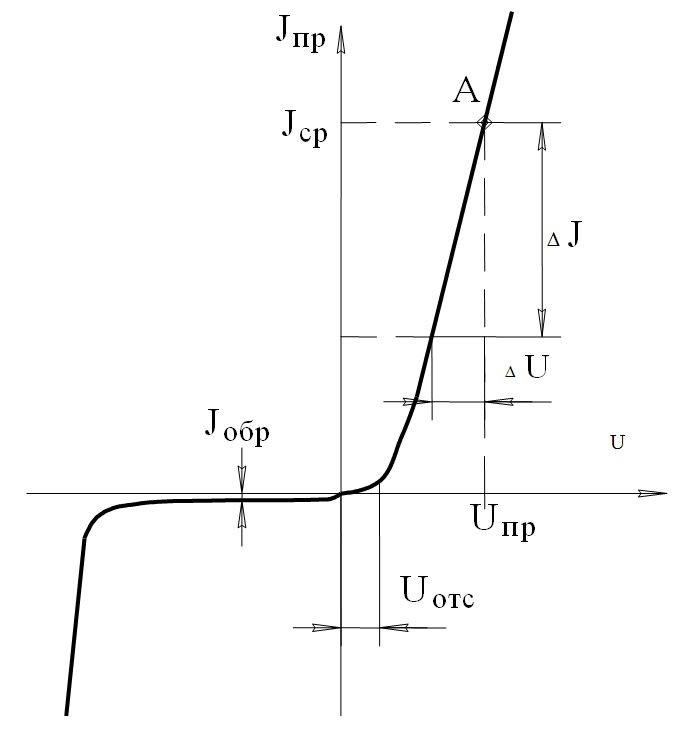
\includegraphics[width=0.4\textwidth]{2_VAC_of_diod.png}
\caption{ВАХ выпрямительного диода}
\label{fig:2_VAC_of_diod}
\end{figure}

\subsection*{Диоды}

Диоды обладают односторонней проводимостью и служат: для выпрямления переменного тока, стабилизации тока и напряжения, формирования импульсов, для регулирования мощностей и т.д.

Выпрямительные диоды применяются для преобразования переменного тока в постоянный. Они делятся: на маломощные (до 0,3А), средней мощности (до 10А), мощные (более 1000А), низкочастотные (до 1кГц) и высокочастотные (до 100кГц).

Свойства выпрямительных диодов характеризуются ВАХ и параметрами, которые приводятся в справочной литературе. Основные параметры диодов: средний выпрямленный ток Jср, прямое падение напряжения Uпр, обратный ток диода при заданной температуре Jобр., напряжение отсечки Uотс., мощность рассеивания Ррас., рабочая частота fр. и др.

\subsection*{Стабилитроны}

Стабилитроны - это разновидность диодов, предназначенных для стабилизации напряжения. Вольт – амперная характеристика стабилитрона имеет вид. Рабочий участок характеристики АВ лежит в области электрического пробоя диода и характеризуется малым изменением напряжения Uст при значительных изменениях тока.

\subsection*{Стабисторы}

Стабисторы, как и стабилитроны, предназначены для стабилизации напряжения. Однако, в отличие от последних, рабочим участком у них является прямая ветвь вольт–амперной характеристики. Стабисторы работают при прямом напряжении и позволяют стабилизировать малые напряжения (0,35 -- 1,9 В).

\subsection*{Варикапы}

Варикапы – это полупроводниковые диоды, емкость которых меняется при изменении обратного напряжения.


% Вопрос 3 ------------------------------------------------------------
\section{Полупроводниковые транзисторы. Классификация. Область применения.}

Транзистор — радиоэлектронный компонент из полупроводникового материала, обычно с тремя выводами, позволяющий входным сигналом управлять током в электрической цепи. Обычно используется для усиления, генерации и преобразования электрических сигналов. В общем случае транзистором называют любое устройство, которое имитирует главное свойство транзистора - изменения сигнала между двумя различными состояниями при изменении сигнала на управляющем электроде. Далее на схеме приведена классификация.

\subsection*{Классификация транзисторов}

\begin{figure}[H]
\centering
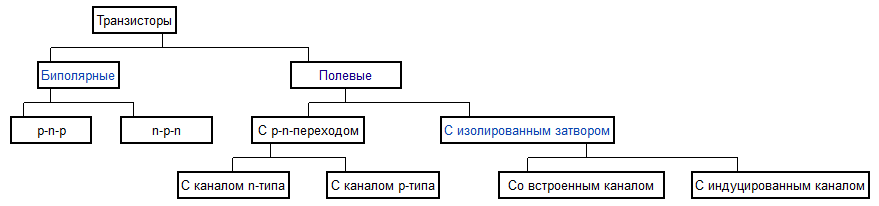
\includegraphics[width=1.0\textwidth]{3_Scheme_of_types.png}
\caption{Классификация транзисторов}
\label{fig:3_Scheme_of_types}
\end{figure}

\subsection*{Биполярный транзистор}

Принцип действия биполярного транзистора основан на использовании физических процессов, происходящих при переносе основных носителей электрических зарядов из эмиттерной области в коллекторную через базу.

$I_\text{э} = I_\text{к} + I_\text{б}$, где $I_\text{э}$, $I_\text{к}$, $I_\text{б}$, – токи соответственно в цепи эмиттера, коллектора, базы.

\subsection*{Полевой транзистор}

Полевым транзистором называется транзистор, в котором между двумя электродами образуется проводящий канал, по которому протекает ток. Управление этим током осуществляется электрическим полем, создаваемым третьим электродом. Электрод, с которого начинается движение носителей заряда, называется истоком, а электрод, к которому они движутся, стоком. Электрод, создающий управляющее электрическое поле, называется затвором.


% Вопрос 4 ------------------------------------------------------------
\section{Полупроводниковые резисторы. Классификация. Область применения.}

Полупроводниковые резисторы нашли широкое применение в электронных приборах. К ним относятся терморезисторы, магниторезисторы, варисторы, фоторезисторы. Принцип действия таких приборов основан на изменении свойств полупроводниковых материалов при воздействии на них температуры, магнитного и электрического полей, электромагнитного излучения.

Полупроводниковый терморезистор представляет собой прибор, сопротивление которого изменяется при изменении температуры. Зависимость сопротивления от температуры имеет вид:

\begin{equation}
R_{T}=A\exp{\frac{B}{T}}\text{, где}
\end{equation}
\par А, В --- постоянные, определяемые свойствами полупроводникового материала и конструкцией терморезистора;
\par Т --- температура.

С увеличением температуры сопротивление терморезистора уменьшается. Температурный коэффициент сопротивления терморезистора лежит в пределах от 2 до 8,5\% на градус.

Недостатком полупроводниковых терморезисторов является нелинейная зависимость сопротивления от температуры и значительный разброс параметров.

Терморезисторы применяются в качестве первичных преобразователей температуры для контроля и регулирования температуры, а также в схемах температурной компенсации.

Магниторезистор представляет собой полупроводниковый прибор, электрическое сопротивление которого зависит от воздействия на него магнитного поля. Магниторезисторы позволяют обеспечить хорошую гальваническую развязку. Для формирования магнитного поля можно использовать постоянный магнит или электромагнит.

Зависимость сопротивления магниторезистора от величины магнитного поля нелинейна. С увеличением величины магнитного поля сопротивление возрастает.

Основными параметрами магниторезистора являются:

\begin{itemize}
\item ном. сопротивление при отсутствии магнитного поля;
\item мощность рассеивания;
\item ТКR (температурный коэффициент сопротивления);
\item зависимость $R_{B} = f(H)$.
\end{itemize}


\begin{figure}[H]
\centering
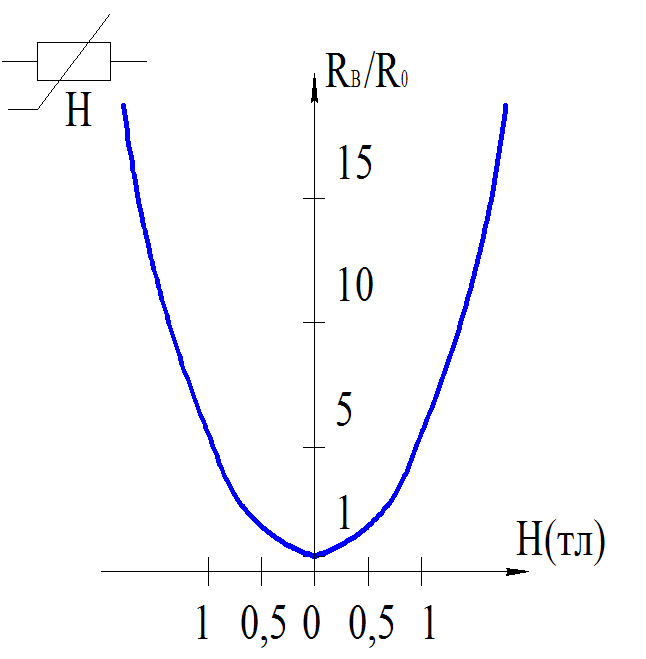
\includegraphics[width=0.35\textwidth]{4_R(H).png}
\hspace{1cm}
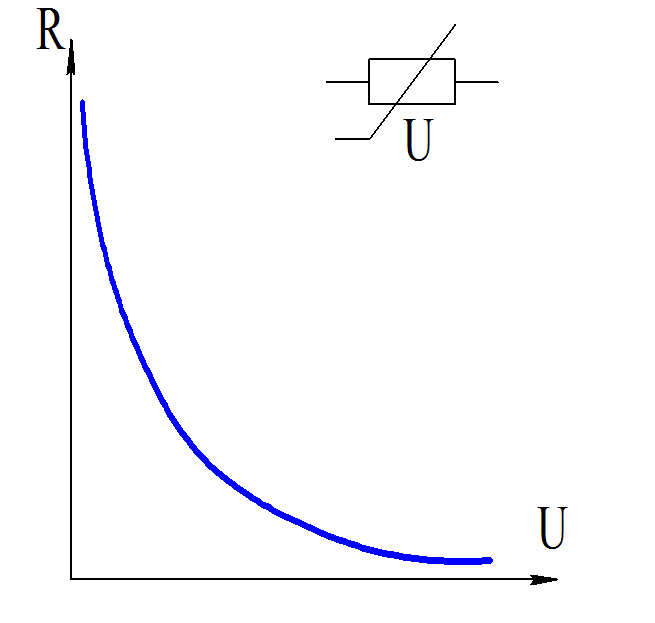
\includegraphics[width=0.35\textwidth]{4_R(U).png}
\\а) \hspace{0.4\textwidth} б)
\caption{Зависимости: R от H (а); R от U (б)}
\label{fig:4_R(U/H)}
\end{figure}

При увеличении магнитной индукции от 0 до 1 Тл сопротивление магниторезистора увеличивается в 10 - 15 раз. Магниторезисторы нашли применение в коммутационной технике: бесконтактных выключателях, реле, контактах управления. В настоящее время в приборостроении нашли широкое применение магнитодиоды, магнитотранзисторы, магнитотиристоры, которые представляют собой полупроводниковые приборы с p-n-переходами, параметры которых чувствительны к магнитному полю.

Варисторы представляют собой полупроводниковые резисторы, сопротивление которых зависит от приложенного напряжения. Зависимость сопротивления от напряжения нелинейная. Сопротивление RВ уменьшается при увеличении приложенного напряжения. Варисторы применяются для защиты от перенапряжений, защиты от помех, для искрогашения в электрических машинах. Они ограничивают возникающее напряжение, особенно при коммутации индуктивной или емкостной нагрузки и тем самым позволяют значительно повысить срок службы контактов реле и т.д.

Фоторезисторы представляют собой полупроводниковые приборы, сопротивление которых зависит от электромагнит. излучения.


% Вопрос 5 ----------------------------------------------------------
\section{Фотоэлектрические приборы. Классификация. Область применения.}

Фотоэлектрические приборы строятся на принципах фотопроводимости.

Фотопроводимость – это свойство веществ изменять свою электропроводность под воздействием электромагнитного излучения.

\subsection*{Классификация фотоэлектронных приборов}

\begin{enumerate}
\item с внешним фотоэффектом
	\begin{itemize}
	\item вакуумные
	\item газонаполненные фотоэлементы (ФЭ)
	\item фотоэлектронные умножители (ФЭУ)
	\end{itemize}
\item с внутренним фотоэффектом
	\begin{itemize}
	\item фоторезисторы
	\item фотодиоды
	\item фототранзисторы
	\item фототиристоры
	\end{itemize}
\end{enumerate}

В качестве излучателей используется солнечный свет, лампочки накаливания и другие источники света.

Фотоэлемент (ФЭ) – это электровакуумный или газоразрядный диод, в стеклянном баллоне которого установлены фотокатод и фотоанод. Фотокатод представляет собой слой, покрывающий внутреннюю поверхность колбы, выполненный из полупроводникового материала, чувствительного к внешнему излучению. Анод выполнен в виде кольца или рамки и размещен внутри колбы. ФЭ разделяются на вакуумные и газоразрядные.

При отсутствии излучения анодный ток равен нулю. При освещении фотокатода возникает фотоэмиссия, и в цепи анода протекает ток.

Фотоэлементы используются в первичных преобразователях информации.

\subsection*{Фотоэлектронный умножитель}

Фотоэлектронный умножитель представляет собой электровакуумный прибор, преобразующий энергию электромагнитного излучения в электрические сигналы с использованием вторичной электронной эмиссии. Состоит из стеклянного баллона, внутри которого расположены ускоряющие электроды, умножительные электроды и анод. При освещении фотокатода возникает электронный поток, который фокусируется и направляется на умножительные электроды, где за счет вторичной эмиссии он усиливается и попадает на анод.

\subsection*{Фоторезистор}

Фоторезистор представляет собой полупроводниковый прибор, сопротивление которого зависит от освещенности.

\subsection*{Фотодиод}

Фотодиод представляет собой полупроводниковый прибор с n-p переходом. Принцип работы фотодиода заключается в том, что при его освещении возрастает обратный ток, и он не зависит от обратного напряжения. На границе перехода “n-p” возникает ЭДС, величина которой зависит от освещенности и может достигать 0,5 - 1 В. При этом обратное сопротивление фотодиода уменьшается.

Они относятся к быстродействующим приборам и реагируют на сигналы до 1 МГц. Фотодиоды могут также использоваться в качестве источников питания, например, в солнечных батареях.

\subsection*{Фототранзистор}

Фототранзистор в отличие от фотодиода является активным преобразователем, в нем происходит не только преобразование энергии излучения, но и усиление.
Внутренний фотоэффект в полупроводнике может быть использован для построения других приборов, например, фототиристоров, однопереходных фототранзисторов и др.


% Вопрос 6 ----------------------------------------------------------------------
\section{Аналоговые усилители. Классификация. Основные характеристики и параметры.}

Усилитель - устройство, предназначенное для усиления электрических сигналов по напряжению, току или мощности за счет преобразования энергии источника питания в энергию выходного сигнала. Усилитель включает в себя нелинейный элемент, управляемый входным электрическим сигналом $U_\text{вх}$, источник питания $U_\text{п}$ и нагрузочное устройство с сопротивлением $Z_\text{н}$. Аналоговые усилители служат для усиления аналоговых сигналов.

\subsection*{Классификация усилителей}

\begin{itemize}
\item по виду усиливаемого:
	\begin{itemize}
	\item гармонических сигналов
	\item импульсных сигналов
	\end{itemize}
\item по типу усиливаемого сигнала:
	\begin{itemize}
	\item напряжения
	\item тока 
	\item мощности
	\end{itemize}
\item по диапазону усиливаемых частот:
	\begin{itemize}
	\item постоянного тока 
	\item переменного тока. Которые в зависимости от диапазона усиливаемых частот делятся на:
		\begin{itemize}
		\item усилители низкой частоты (УНЧ)
		\item высокой частоты (УВЧ)
		\item широкополосные
		\item избирательные усилители.
		\end{itemize}
	\end{itemize}
\item по виду нагрузки:
	\begin{itemize}
	\item с активной нагрузкой
	\item c активно-индуктивной нагрузкой
	\item c емкостной нагрузкой
	\end{itemize}
\item по количеству каскадов:
	\begin{itemize}
	\item однокаскадные 
	\item многокаскадные. Связь в между каскадами может быть:
		\begin{itemize}
		\item гальванической
		\item емкостной
		\item индуктивной
		\end{itemize}
	\end{itemize}
\end{itemize}

\subsection*{Основные характеристики усилителя}

\begin{itemize}
\item амплитудная характеристика, которая представляет собой зависимость $U_\text{выx} = \varphi(U_\text{вх})$. Для линейных усилителей это прямая, проходящая через начало координат;
\item амплитудно-частотная характеристика (АЧХ) $U_\text{выx} = \varphi(f)$ отражает зависимость амплитуды выходного сигнала от частоты. Реально в усилителях из-за наличия паразитных емкостей и индуктивностей различные частоты усиливаются неодинаково;
\item фазо-частотная характеристика $U_\text{выx} = \lambda(f)$ отражает зависимость угла сдвига фазы выходного сигнала по отношению к фазе входного сигнала;
\item переходная характеристика – отражает реакцию усилителя на единичный скачок входного напряжения. Переходная характеристика определяется по ее изображению на экране осциллографа при подаче на вход усилителя входного сигнала прямоугольной формы. Процесс изменения выходного сигнала может быть колебательным либо апериодичным.
\end{itemize}

\subsection*{Важнейшие параметры усилителя}

\begin{itemize}
\item коэффициент усиления по току $K_{I} = \dfrac{\Delta I_\text{вых}}{\Delta I_\text{вх}}$
\item коэффициент усиления по напряжению $K_{U} = \dfrac{\Delta U_\text{вых}}{\Delta U_\text{вх}}$
\item коэффициент усиления по мощности $K_{P} = \dfrac{\Delta P_\text{вых}}{\Delta P_\text{вх}}$
\item Полоса пропускания усилителя $2\Delta f$ характеризует частотные свойства усилителя. Измеряется на уровне $0,707 K_{max}$
\end{itemize}

Для наглядности в ряде случаев АЧХ строится в относительных единицах усиления.
\begin{equation}
N(F) = \dfrac{K(f)}{K_{max}}\text{, где}
\end{equation}
\par $K(f)$ --- коэффициент усиления на частоте $f$;
\par $K_{max}$ --- максимальный коэффициент усиления.

Входное и выходное сопротивление необходимо учитывать при согласовании с источником входного сигнала и с нагрузкой. 

Выходная мощность усилителя – это мощность, которая выделяется на нагрузке.

Искажения сигналов в усилителе – это отклонение формы выходного сигнала от формы входного сигнала. Различают два вида искажений: статические (нелинейные) и динамические (линейные). Нелинейные искажения возникают в усилителе за счет работы его на нелинейном участке ВАХ. Количественно нелинейные искажения оцениваются коэффициентом нелинейных искажений.

\begin{equation}
K_{H} = \dfrac{\sqrt{(A_{2}^{2} + A_{3}^{2} + \ldots + A_{n}^{2})} }{A_{1}}\text{, где}
\end{equation}
\par $A_{n}$ --- амплитуда n-й гармоники;
\par $A_{1}$ --- амплитуда основной гармоники выходного сигнала.

Линейные искажения определяются амплитудно-частотной характеристикой усилителя и количественно оцениваются коэффициентами частотных искажений на низких и высоких частотах.

Для получения высоких коэффициентов усиления в состав усилителя входит обычно несколько каскадов. Первым каскадом, как правило, является предварительный усилитель, затем идут промежуточный усилитель и усилитель мощности. Предварительный усилитель обеспечивает связь источника сигнала с усилителем. Он должен иметь большое входное сопротивление для того, чтобы не ослаблять входной сигнал. Промежуточный усилитель обеспечивает основное усиление, а усилитель мощности обеспечивает заданную выходную мощность.

При построении усилительных устройств наибольшее распространение получили каскады на биполярных и полевых транзисторах, включенных с ОЭ (OU) или с ОК (OC).

% Вопрос 7 -----------------------------------------------------------------------------------------
\section{Избирательные усилители. Усилители постоянного тока. Усилители мощности. Область применения.}

Избирательными называются усилители, усиливающие сигналы в относительно узкой полосе частот. Основными показателями избирательных усилителей являются максимальный коэффициент усиления, полоса пропускания, средняя частота полосы пропускания и избирательность. Основным требованием, предъявляемым к избирательным усилителям, является получение высокой избирательности, которая определяется крутизной склонов его амплитудно-частотной характеристики. Чем круче спады частотной характеристики и чем меньше коэффициент усиления усилителя за пределами полосы пропускания, тем выше его избирательность. Избирательность таких усилителей оценивают величиной коэффициента прямоугольности АЧХ, который равен отношению ширины полосы пропускания на уровне 0,7 к ширине полосы на уровне 0,1 (или к ширине полосы на уровне 0,01):

\begin{equation}
K_\text{п} = \dfrac{2\Delta f_{0,7}}{2\Delta f_{0,01 - 0,1}}
\end{equation}

Избирательные усилители применяются в основном для усиления сигналов высокой частоты и разделяются на два вида: резонансные усилители и полосовые усилители. В резонансных усилителях нагрузкой обычно является одиночный параллельный колебательный контур. Перестраивая контур, можно изменять резонансную частоту в некоторых пределах.

Полосовые усилители обеспечивают амплитудно-частотную характеристику по форме близкую к прямоугольной. Полосовые усилители не перестраиваются и работают на фиксированных частотах. В качестве нагрузки они имеют один или два колебательных контура в каждом каскаде. В усилителях промежуточной частоты радиоприемников применяются также фильтры сосредоточенной селекции, состоящие из трех-четырех связанных колебательных контуров. В качестве фильтров сосредоточенной селекции также широко применяются пьезоэлектрические фильтры. В них благодаря прямому и обратному пьезоэлектрическому эффекту амплитудно-частотная характеристика формируется в системе из нескольких механических резонаторов.

Однокаскадный резонансный усилитель состоит из активного элемента, нагрузкой которого является одиночный параллельный колебательный контур. В качестве активного элемента можно использовать биполярные или полевые транзисторы, включаемые, чаще всего, по схеме с общим эмиттером или общим истоком. При этом колебательный контур оказывается зашунтированным выходным сопротивлением собственного каскада и входным сопротивлением следующего каскада в многокаскадном усилителе, за счет чего избирательность ухудшается. В каскадах с полевым транзистором колебательный контур шунтируется слабо, так как входное и выходное сопротивление полевого транзистора достаточно большое. В таких каскадах возможно полное включение контура в нагрузочную цепь. Биполярные транзисторы имеют относительно малые значения входных и выходных сопротивлений. Поэтому при непосредственном включении колебательного контура в нагрузочную цепь контур шунтируется значительно сильнее и его избирательные свойства заметно ухудшаются. Поэтому в резонансных каскадах на биполярных транзисторах принимают специальные меры для уменьшения шунтирующего действия входного и выходного сопротивления транзистора. С этой целью ослабляют связь транзистора с колебательным контуром, используя частичное включение контура в нагрузочную цепь. В связи с тем, что резонансные избирательные усилители работают на высокой частоте, существенное влияние на их работу может оказывать внутренняя обратная связь, имеющаяся между входом и выходом в любом активном элементе. Эта внутренняя обратная связь на одной из высоких частот может оказаться положительной, что приведет к нарушению устойчивой работы усилителя и его самовозбуждению. Для повышения устойчивости работы каскада необходимо ослаблять связь его активного элемента с колебательным контуром. С этой целью частичное включение контура используют и в резонансных каскадах на полевых транзисторах. Далее на рисунке показана схема резонансного усилителя на полевом транзисторе с полным включением контура и его АЧХ.

\subsection*{Схема на полевом транзисторе}

Модуль коэффициента усиления каскада на полевом транзисторе при полном включении контура примерно равен:

\begin{equation}
|K_\text{рез}| \approx S R_\text{рез}
\end{equation}
где $ R_\text{рез} = Q\rho $ - сопротивление параллельного контура на резонансной частоте.

\begin{figure}[H]
\centering
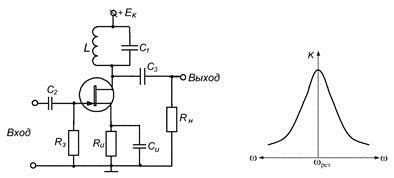
\includegraphics[width=0.6\textwidth]{7_field_based_amp.jpg}
\caption{Избирательный усилитель на полевом транзисторе и его АЧХ}
\label{fig:7_field_based_amp}
\end{figure}

\subsection*{Схема на биполярном транзисторе}

Далее показана схема избирательного усилителя на биполярном транзисторе с неполным включением контура. Для каскада на биполярном транзисторе при неполном включении контура в цепь нагрузки необходимо учитывать коэффициенты подключения контура и модуль коэффициента усиления будет определяться следующим выражением:

\begin{equation}
|K_\text{рез}| = b_{1}b_{2} \dfrac{\beta R_\text{рез}}{R_\text{вх}}
\end{equation}
где $ b_{1} = \dfrac{L\prime}{L} $ и $ b_{2} = \dfrac{L\prime\prime}{L} $ - коэффициенты включения контура; $L$ - полная индуктивность катушки; $L\prime$ - индуктивность части катушки, к которой подключен коллектор транзистора; $L\prime\prime$ - индуктивность части катушки, с которой усиленный сигнал снимается на вход следующего каскада.

\begin{figure}[H]
\centering
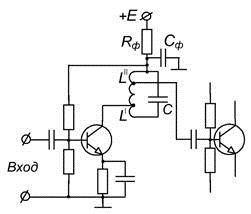
\includegraphics[width=0.4\textwidth]{7_bipolar_based_amp.jpg}
\caption{Избирательный усилитель на биполярном транзисторе}
\label{fig:7_bipolar_based_amp}
\end{figure}

\subsection*{2T-мост}

При необходимости избирательного усиления низких частот емкости и индуктивности колебательного контура должны быть большими и добротность контура оказывается низкой при значительном увеличении габаритов катушки и конденсатора. Поэтому в качестве низкочастотных избирательных усилителей используют усилители с частотно-зависимой отрицательной обратной связью. В качестве частотно-зависимой цепи используют двойной T-образный мост (2T-мост).

\begin{figure}[H]
\centering
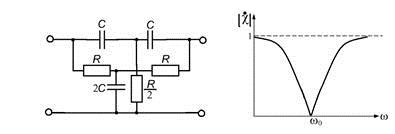
\includegraphics[width=0.6\textwidth]{7_2T.jpg}
\caption{Схема 2T-моста и АХЧ}
\label{fig:7_2T}
\end{figure}

Если включить 2T-мост в цепь отрицательной обратной связи в RC-усилитель, то поскольку на частоте $\omega = \omega_{0}$ коэффициент передачи моста равен нулю, отрицательная обратная связь будет отсутствовать, и коэффициент усиления усилителя будет максимальным. На всех остальных частотах коэффициент усиления избирательно уменьшается из-за наличия отрицательной обратной связи. В результате амплитудно-частотная характеристика усилителя с 2T-мостом в цепи отрицательной обратной связи будет иметь ярко выраженный максимум на частоте $\omega_{0}$.

\begin{figure}[H]
\centering
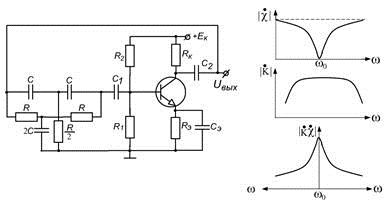
\includegraphics[width=0.6\textwidth]{7_2T_with_feedback.jpg}
\caption{Схема 2T-моста с обратной связью и АХЧ}
\label{fig:7_2T_with_feedback}
\end{figure}

Схема избирательного усилителя с 2T-мостом эквивалентна резонансному каскаду, имеющему добротность $Q = \dfrac{K}{4}$ , где $K$- коэффициент усиления усилителя без обратной связи. Для увеличения эквивалентной добротности избирательной системы можно цепью отрицательной обратной связи через 2Т-мост охватывать несколько каскадов усиления.

\subsection*{Усилители постоянного тока}

Усилителями постоянного тока называют такие устройства, которые могут усиливать медленно изменяющиеся электрические сигналы, то есть они способны усиливать и переменные и постоянные составляющие входного сигнала. Усилители постоянного тока имеют много разновидностей (дифференциальные, операционные, усилители с преобразованием входного сигнала и др.). Поскольку такие устройства пропускают наряду с переменной составляющей еще и постоянную, то отдельные каскады должны быть связаны между собой либо непосредственно, либо через резисторы, но не через разделительные конденсаторы или трансформаторы, которые не пропускают постоянную составляющую. Основную проблему усилителей постоянного тока представляет дрейф нуля – отклонение напряжения на выходе усилителя от начального (нулевого) значения при отсутствии входного сигнала. Основной причиной этого явления являются температурная и временная нестабильность параметров активных элементов схемы усилителя, резисторов, а также источников питания. Одним из возможных путей уменьшения дрейфа нуля является использование дифференциальных усилителей.

\begin{itemize}
\item Дифференциальные усилители предназначены для усиления сколь угодно медленно изменяющихся во времени сигналов, частотный диапазон которых начинается от 0 Гц.
\item Дифференциальный усилитель: имеет следующие достоинства: малый дрейф нуля; высокая степень подавления синфазных помех.
\item Недостатки дифференциального усилителя: требует двухполярного источника питания; необходима очень высокая симметрия схемы.
\end{itemize}

\begin{figure}[H]
\centering
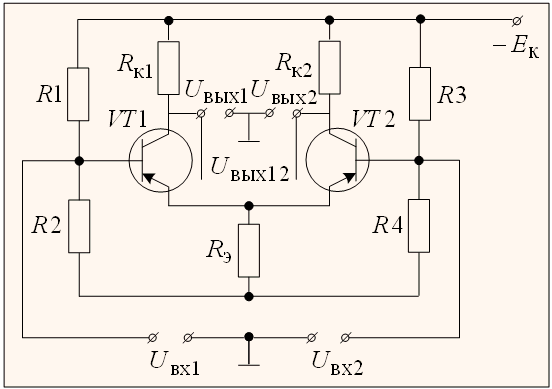
\includegraphics[width=0.5\textwidth]{7_diff_amp.png}
\caption{Схема простейшего дифференциального усилителя}
\label{fig:7_diff_amp}
\end{figure}

\begin{itemize}
\item Дифференциальные усилители предназначены для усиления сколь угодно медленно изменяющихся во времени сигналов, частотный диапазон которых начинается от 0 Гц.
\item Дифференциальный усилитель: имеет следующие достоинства: малый дрейф нуля; высокая степень подавления синфазных помех.
\item Недостатки дифференциального усилителя: требует двухполярного источника питания; необходима очень высокая симметрия схемы.
\end{itemize}


% Вопрос 8 ------------------------------------------------------------------------
\section{Операционные усилители. Классификация. Область применения. Балансировка ОУ.}

Операционным усилителем называют усилитель постоянного тока, предназначенный для выполнения различного рода операций над аналоговыми сигнала при работе в схемах с отрицательной обратной связью.

Операционные усилители обладают большим и стабильным коэффициентом усиления напряжения, имеют дифференциальный вход с высоким входным сопротивлением и несимметричный выход с низким выходным сопротивлением, малым дрейфом нуля. То есть под операционным усилителем понимают высококачественный универсальный усилитель.

Условные обозначения операционных усилителей приведены ниже. Один из входов, обозначенный знаком «+» называют неинвертирующим (прямым), так как сигнал на выходе и сигнал на этом входе имеют одинаковую полярность. Второй вход, обозначенный знаком «–», (его также обозначают знаком инверсии «o») называют инвертирующим, так как сигнал на выходе по отношению к сигналу на этом входе имеет противоположную полярность. Помимо трех сигнальных контактов (двух входных и одного выходного) операционный усилитель содержит дополнительные контакты (обычно число контактов составляет 14 или 16).

\begin{figure}[H]
\centering
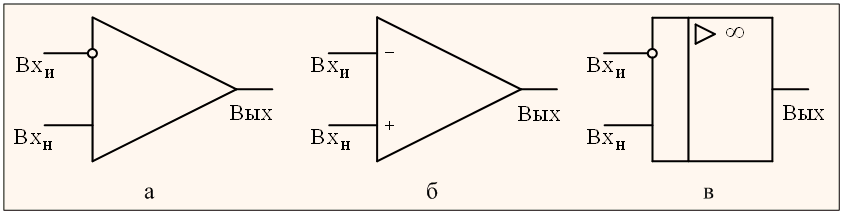
\includegraphics[width=0.7\textwidth]{8_oa_graphic.png}
\caption{УГО операционного усилителя}
\label{fig:8_oa_graphic}
\end{figure}

\subsection*{Основные параметры}

\begin{enumerate}
\item Коэффициент усиления напряжения без обратной связи $K_{u}$, показывающий, во сколько раз напряжение на выходе превышает напряжение сигнала, поданного на дифференциальный вход. Типовое значение $K_{u} = 10^{5} \div 10^{6}$;
\item Коэффициент ослабления синфазного сигнала $K_\text{осл.сф}$, показывающий, во сколько раз дифференциальный сигнал сильнее синфазного. Донный параметр определяется свойствами входного дифференциального каскада и составляет $80 \div 100$ дБ;
\item Напряжение смещения нуля $U_\text{см}$, представляющее собой постоянное напряжение определенной полярности, которое необходимо подать на вход при отсутствии входного сигнала для того, чтобы напряжение на выходе стало равным нулю. Наличие отклонения выходного напряжения от нуля обусловлено, хотя и малым, но неизбежным дисбалансом плеч дифференциального каскада. Практически $U_\text{см} = 5 \div 20$ мВ;
\item Температурный дрейф напряжения смещения $TKU_\text{см} = \dfrac{\Delta U_\text{см}}{\Delta T}$, характеризует изменение напряжения $U_\text{см}$ при изменении температуры и составляет $1 \div 30 \dfrac{\text{мкВ}}{\text{\textcelsius}}$;
\item Входное сопротивление для дифференциального сигнала $R_\text{вх. диф}$. Измеряется со стороны любого входа в то время, когда другой вход соединен с общим выводом. Величина $R_\text{вх. диф}$ лежит в пределах сотен кОм – единиц МОм;
\item Входное сопротивление для синфазного сигнала $R_\text{вх. сф}$. Измеряется между соединенными вместе входами операционного усилителя и корпусом. Данное сопротивление на несколько порядков больше чем сопротивление для дифференциального сигнала;
\item Выходное сопротивление $R_\text{вых}$. Величина выходного сопротивления для операционного усилителя составляет десятки – сотни Ом.
\end{enumerate}

\subsection*{Виды ОУ}

\begin{enumerate}
\item Универсальные усилители общего назначения составляют большую часть номенклатуры ОУ. Это дешевые усилители среднего быстродействия, невысокой точности и малой выходной мощности, с  типичными параметрами: Ku = $10^{3} - 10^{5}$, f1 = 0.1 - 10 МГц и напряжение смещения нулевого уровня Uсм = 0.1 - 10 мВ.
\item Прецизионные усилители характеризуются суммарной погрешностью не более долей процента и при среднем быстродействии имеют высокий коэффициент усиления напряжения, малое напряжение смещения нуля, большой коэффициент подавления синфазного сигнала, малый входной ток и низкий уровень шума.
\item Быстродействующие усилители имеют высокую частоту единичного усиления f1 = 50 - 1000 МГц и обеспечивают скорость нарастания выходного сигнала Vu= 10 - 1000 В/мкс при средних точностных параметрах.
\item Микромощные усилители потребляют очень малый ток Iпит порядка 1 мкА при небольших уровнях напряжения электропитания Uпит = $\pm 0.9 - \pm 5$ В. Все другие параметры (особенно быстродействие) у них обычно невысокие. Эти усилители используют в приборах с автономным электропитанием от гальванических или аккумуляторных батарей.
\item Мощные и высоковольтные усилители имеют разность положительного и отрицательного питающих напряжений свыше 50 В и выходной ток 0.1 - 1А, а некоторые модификации допускают токи до 10 - 100 А и мощности свыше 100 Вт.
\end{enumerate}

\subsection*{Балансировка ОУ}

ОУ имеет два вывода балансировки (на рисунке обозначены Offset), которые обеспечивают возможность подстройки напряжения смещения входа ОУ до нулевого значения. Для подстройки нужно подключить к выводам потенциометр.


% Вопрос 9 --------------------------------------------------------------------
\section{Стабилизаторы напряжения. Классификация. Параметры. Область применения.}

Стабилизатор напряжения — преобразователь электрической энергии, позволяющий получить на выходе напряжение, находящееся в заданных пределах при значительно больших колебаниях входного напряжения и сопротивления нагрузки.

По типу выходного напряжения стабилизаторы делятся на стабилизаторы постоянного тока и переменного тока. Как правило, тип питания (постоянный либо переменный ток) такой же, как и выходное напряжение, хотя возможны исключения.

Стабилизаторы напряжения подразделяются на однофазные и трехфазные стабилизаторы напряжения.

\subsection*{Классификация стабилизаторов по конструкции}

\begin{itemize}
\item феррорезонансные. Принцип действия основывается на магнитном насыщении сердечников из ферромагнетиков трансформаторов. Этот тип стабилизаторов напряжения был разработан достаточно давно, в начале 60-х годов прошлого века и был призван защитить сложную бытовую технику. Но в настоящее время от их производства отказались почти все производители, из-за очень узкого рабочего диапазона напряжений и невозможности работы прибора без нагрузки.
\item электромеханические. В стабилизаторах этого типа корректировка напряжения производится автоматически, а точность поддержания напряжения достаточно высока (в пределах 3\%).
\item электронные. Этот тип стабилизаторов работает по принципу автоматического переключения трансформаторных секций при помощи силовых ключей (реле, тиристоров и т.д.). Электронные стабилизаторы ступенчатого регулирования обеспечивают выходное напряжение в более широких пределах, чем электромеханические. А также обладают высоким быстродействием и не изменяют форму входного напряжения.
\end{itemize}

\subsection*{Основные параметры стабилизатора}

\begin{itemize}
\item Диапазон входных напряжений(Диапазон напряжений в пределах которого стабилизатор может поддерживать выходное напряжение с заданной точностью)
\item Диапазон  выходных напряжений (Диапазон возможных значений)
\item Точность поддержания выходного напряжения в \%
\item Мощность стабилизатора. Обычно указывается в кВа, это полная мощность.
\end{itemize}

\subsection*{Выбор стабилизатора}

\begin{enumerate}
\item Для выбора стабилизатора необходимо посчитать сумму полных мощностей потребителей, если на потребителе указан $\cos\varphi$ (коэфф. активном мощности в полной), то его учитываем.
\item Определить диапазон изменений напряжений в сети. Произвести изменения максимальных и минимальных напряжений.
\item Выяснить диапазон рабочих напряжений потребителей
\end{enumerate}


% Вопрос 10 ------------------------------------
\section{Логические операции. Схемная реализация.}

Логическая операция — операция над выражениями булевского типа, соответствующая некоторой операции над высказываниями в алгебре логики. Как и высказывания, логические выражения могут принимать одно из двух истинностных значений — «истинно» или «ложно». Логические операции служат для получения сложных логических выражений из более простых. В свою очередь, логические выражения обычно используются как условия для управления последовательностью выполнения программы.
Обычно выделяют следующие базовые операции:

\begin{itemize}
\item НЕ (отрицание)
\item И (конъюнкция)
\item ИЛИ (дизъюнкция)
\item XOR (исключающее ИЛИ)
\end{itemize}

Для каждой из операции можно построить простую таблицу истинности.

\begin{figure}[H]
\centering
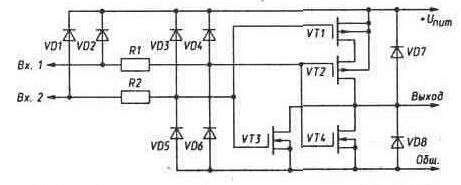
\includegraphics[width=0.7\textwidth]{10_or_not.png}
\caption{Схемная реализация ИЛИ-НЕ}
\label{fig:10_or_not}
\end{figure}

Для всех микросхем существует УГО.


% Вопрос 11 ---------------------------------------------------------------------------------------------------------------
\section{Цифровые устройства. Классификация. Комбинационные ЦУ. Дешифраторы, шифраторы, мультиплексоры, демультиплексоры.}

\subsection*{Виды цифровых устройств}

\begin{enumerate}
\item Логические элементы
\item Триггеры
\item Счётчики
\item Регистры
\item Буферные преобразователи
\item Модули памяти
\item Шифраторы
\item Дешифраторы
\item Цифровой компаратор
\item Мультиплексоры
\item Демультиплексоры
\item Полусумматоры
\item Сумматоры
\item АЛУ
\item Микроконтроллеры
\item (Микро)процессоры
\item Однокристальные микрокомпьютеры
\item ПЛИС — программируемые логические интегральные схемы
\end{enumerate}

\subsection*{Классификация цифровых устройств}

\begin{itemize}
\item В зависимости от способа  ввода и вывода информации:
	\begin{itemize}
	\item Последовательные – в котором входные сигналы поступают на вход, а выходные сигналы снимаются с выхода последовательно, разряд за разрядом;
	\item Параллельные – входные сигналы подаются на вход, а выходные снимаются с выхода одновременно;
	\item Последовательно-параллельные – входные и выходные сигналы представлены в разных формах: либо на вход сигналы поступают последовательно сигнал за сигналом, а с выхода они снимаются одновременно, и наоборот.
	\end{itemize}
\item По принципу действия:
	\begin{itemize}
	\item КЦУ (комбинационные цифр.устр-ва) – выходные сигналы которых определяются только действующими в данный момент входными сигналами и не зависят от внутреннего состояния устройства.
	\item Последовательными – выходные сигналы которых зависят не только от входных сигналов, но и от внутреннего состояния устройства. Этот тип называют цифровыми автоматами.
	\end{itemize}
\end{itemize}

\subsection*{Виды комбинационных ЦУ}
\begin{itemize}
\item дешифраторы
\item шифраторы
\item мультиплексоры
\item демультиплексоры
\item комбинационные сумматоры
\item АЛУ
\end{itemize}


\subsection*{Дешифратор}

Дешифратором называется комбинационная цифровая схема с несколькими входами и выходами, преобразующая код, подаваемый на входы, в сигнал на одном из выходов. Если дешифратор, имеющий n входов, имеет $2^{n}$ выходов, то такой дешифратор называется полным. Если количество выходов меньше, то дешифратор называется неполным.
\begin{figure}[H]
\centering
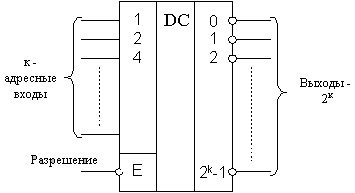
\includegraphics[width=0.5\textwidth]{11_dc.png}
\caption{УГО дешифратора}
\label{fig:11_dc}
\end{figure}

\subsection*{Шифратор}

Шифратором называется устройство, предназначенное для преобразования чисел из десятичной системы в двоичную. Нетрудно видеть, что в шифраторе сигнал, подаваемый на вход X0, не используется. Основное применение шифраторов - это введение первичной информации с клавиатуры (преобразование десятичного в ДВОИЧНЫЙ), например, ИС К555ИВЗ.
\begin{figure}[H]
\centering
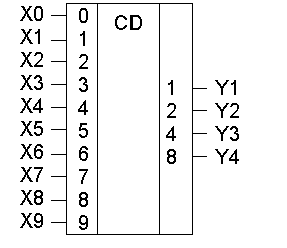
\includegraphics[width=0.4\textwidth]{11_cd.png}
\caption{УГО шифратора}
\label{fig:11_cd}
\end{figure}

\subsection*{Мультиплексор}

Мультиплексором называется комбинационное цифровое устройство, предназначенное для управляемой передачи информации с нескольких источников в один выходной канал. Мультиплексор можно реализовать, используя логические элементы "И" и дешифратор. Мультиплексор имеет один выход, информационные входы и адресные или управляющие входы. В зависимости от кода, подаваемого на адресные шины Х0, Х1 один из информационных входов подключается к выходному каналу.
\begin{figure}[H]
\centering
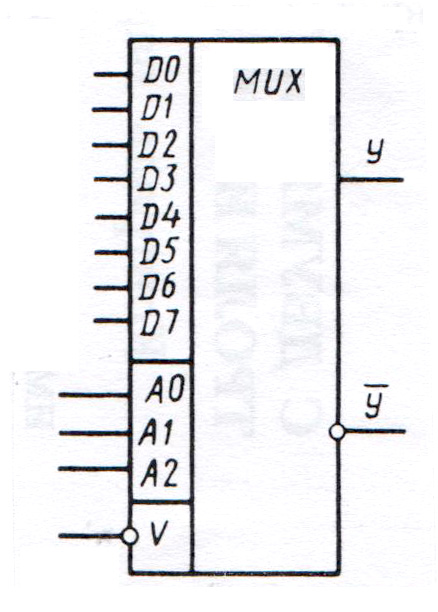
\includegraphics[width=0.25\textwidth]{11_ms.jpg}
\caption{УГО мультиплексора}
\label{fig:11_ms}
\end{figure}

\subsection*{Демультиплексор}

Демультиплексором называется комбинационное логическое устройство, предназначенное для управляемой передачи данных от одного источника информации в несколько выходных каналов. Демультиплексор имеет один информационный вход, n адресных шин и $2^{n}$-выходов.
\begin{figure}[H]
\centering
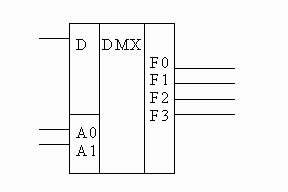
\includegraphics[width=0.45\textwidth]{11_dmx.png}
\caption{УГО демультиплексора}
\label{fig:11_dmx}
\end{figure}


% Вопрос 12 ---------------------------------------------------------------------------------------------------------------
\section{Комбинационные сумматоры.}

Комбинационный сумматор - это цифровое устройство, пред-назначенное для арифметического сложения чисел, представленных в виде двоичных кодов.

Обычно сумматор представляет собой комбинацию одноразрядных сумматоров. При сложении двух чисел в каждом разряде производится сложение трех цифр: цифры первого слагаемого Ai, цифры второго слагаемого Bi; и цифры переноса из младшего разряда Рi;. В результате суммирования на выходных шинах получается сумма S; и перенос в старший разряд Pj+i.

\begin{figure}[H]
\centering
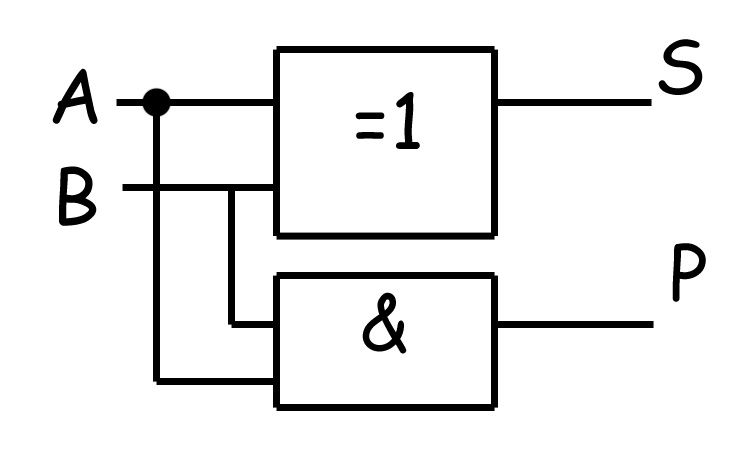
\includegraphics[width=0.3\textwidth]{12_additor.jpg}
\caption{Структура простейшего сумматора}
\label{fig:12_additor}
\end{figure}

\begin{figure}[H]
\centering
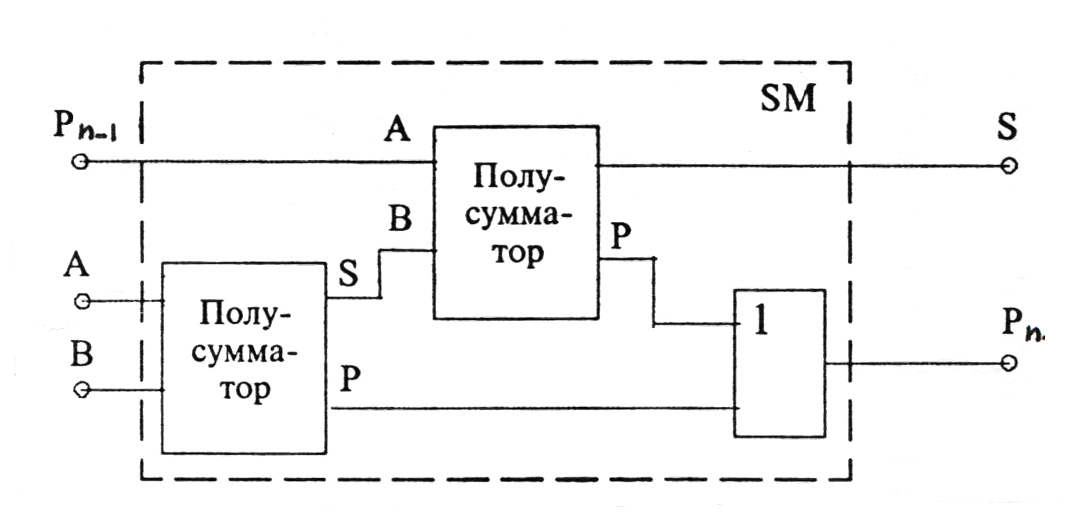
\includegraphics[width=0.7\textwidth]{12_cs.jpg}
\caption{Структура комбинационного сумматора}
\label{fig:12_cs}
\end{figure}


% Вопрос 13 ---------------------------------------------------------------------------------------------------------------
\section{Триггера. Классификация. Область применения.}

Триггером называется цифровое устройство, которое может находиться в одном из двух устойчивых состояний и переходит из одного состояния в другое под действием входных сигналов. Триггеры можно классифицировать по способу приема информации, принципу построения, функциональным возможностям. По способу приема информации триггеры подразделяются на асинхронные и синхронные. Асинхронный триггер изменяет свое состояние в момент прихода сигнала на его информационные входы. Синхронные триггеры изменяют свое состояние под воздействием входных сигналов только в момент прихода активного сигнала на его синхронизирующий вход С.

По виду активного сигнала, действующего на информационных входах, триггеры подразделяются на статические и динамические. Первые переключаются потенциалом (уровнем напряжения), а вторые – перепадом (передним или задним фронтом импульса). Входные информационные сигналы могут быть прямыми и инверсными.

\subsection*{Асинхронный RS-триггер}

RS-триггер — триггер, который сохраняет своё предыдущее состояние при нулевых входах и меняет своё выходное состояние при подаче на один из его входов единицы.

Таблица истинности асинхронного RS-триггера.

\begin{tabular}{|c|c|c|}
\hline	S	& R	& Q			\\
\hline	0	& 0	& Q(n-1)	\\
\hline	0	& 1	& 0			\\
\hline	1	& 0	& 1			\\
\hline	1	& 1	& X			\\
\hline
\end{tabular}

\subsection*{Синхронный RS-триггер}

Синхронный RS-триггер очень похож на асинхронный, с тем лишь различием, что имеется вход синхронизации, при 1 на котором и происходит работа.

Таблица истинности синхронного RS-триггера.

\begin{tabular}{|c|c|c|c|c|}
\hline	C	& S	& R	& Q(t)	& Q(t+1)	\\
\hline	0	& X	& X	& 0		& 0			\\
\hline	0	& X	& X	& 1		& 1			\\
\hline	1	& 0	& 0	& 0		& 0			\\
\hline	1	& 0	& 0	& 1		& 1			\\
\hline	1	& 0	& 1	& 0		& 0			\\
\hline	1	& 0	& 1	& 1		& 0			\\
\hline	1	& 1	& 0	& 0		& 1			\\
\hline	1	& 1	& 0	& 1		& 1			\\
\hline	1	& 1	& 1	& 0		& не опред.	\\
\hline	1	& 1	& 1	& 1		& не опред.	\\
\hline
\end{tabular}

\subsection*{D-триггер}

D-триггер — запоминает состояние входа и выдаёт его на выход. D-триггеры имеют, как минимум, два входа: информационный D и синхронизации С. После прихода активного фронта импульса синхронизации на вход С D-триггер открывается. Сохранение информации в D-триггерах происходит после спада импульса синхронизации С. Так как информация на выходе остаётся неизменной до прихода очередного импульса синхронизации, D-триггер называют также триггером с запоминанием информации или триггером-защёлкой. Рассуждая чисто теоретически, парафазный (двухфазный) D-триггер можно образовать из любых RS- или JK-триггеров, если на их входы одновременно подавать взаимно инверсные сигналы.

D-триггер в основном используется для реализации защёлки. Так, например, для снятия 32 бит информации с параллельной шины, берут 32 D-триггера и объединяют их входы синхронизации для управления записью информации в защёлку, а 32 D входа подсоединяют к шине.

В одноступенчатых D-триггерах во время прозрачности все изменения информации на входе D передаются на выход Q. Там, где это нежелательно, нужно применять двухступенчатые (двухтактные, Master-Slave, MS) D-триггеры.

Таблица истинности синхронного D-триггера.

\begin{tabular}{|c|c|c|}
\hline	D	& Q(t)	& Q(t+1)	\\
\hline	0	& 0		& 0			\\
\hline	0	& 1		& 0			\\
\hline	1	& 0		& 1			\\
\hline	1	& 1		& 1			\\
\hline
\end{tabular}

\subsection*{T-триггер}

Синхронный Т-триггер, при единице на входе Т, по каждому такту на входе С изменяет своё логическое состояние на противоположное, и не изменяет выходное состояние при нуле на входе T. Т-триггер можно построить на JK-триггере, на двухступенчатом (Master-Slave, MS) D-триггере и на двух одноступенчатых D-триггерах и инверторе.

Как можно видеть в таблице истинности JK-триггера, он переходит в инверсное состояние каждый раз при одновременной подаче на входы J и K логической 1. Это свойство позволяет создать на базе JK-триггера Т-триггер, объединяя входы J и К.

В двухступенчатом (Master-Slave, MS) D-триггере инверсный выход Q соединяется со входом D, а на вход С подаются счётные импульсы. В результате триггер при каждом счётном импульсе запоминает значение Q, то есть будет переключаться в противоположное состояние.

Т-триггер часто применяют для понижения частоты в 2 раза, при этом на Т вход подают единицу, а на С — сигнал с частотой, которая будет поделена на 2.

Таблица истинности синхронного T-триггера.

\begin{tabular}{|c|c|c|}
\hline	T	& Q(t)	& Q(t+1)	\\
\hline	0	& 0		& 0			\\
\hline	0	& 1		& 1			\\
\hline	1	& 0		& 1			\\
\hline	1	& 1		& 0			\\
\hline
\end{tabular}

\subsection*{JK-триггер}

JK-триггер работает так же как RS-триггер, с одним лишь исключением: при подаче логической единицы на оба входа J и K состояние выхода триггера изменяется на противоположное. Вход J (от англ. Jump — прыжок) аналогичен входу S у RS-триггера. Вход K (от англ. Kill — убить) аналогичен входу R у RS-триггера. При подаче единицы на вход J и нуля на вход K выходное состояние триггера становится равным логической единице. А при подаче единицы на вход K и нуля на вход J выходное состояние триггера становится равным логическому нулю. JK-триггер в отличие от RS-триггера не имеет запрещённых состояний на основных входах, однако это никак не помогает при нарушении правил разработки логических схем. На практике применяются только синхронные JK-триггеры, то есть состояния основных входов J и K учитываются только в момент тактирования, например по положительному фронту импульса на входе синхронизации.

На базе JK-триггера возможно построить D-триггер или Т-триггер. Как можно видеть в таблице истинности JK-триггера, он переходит в инверсное состояние каждый раз при одновременной подаче на входы J и K логической 1. Это свойство позволяет создать на базе JK-триггера Т-триггер, объединив входы J и К.

Таблица истинности синхронного JK-триггера.

\begin{tabular}{|c|c|c|c|}
\hline	J	& K	& Q(t)	& Q(t+1)	\\
\hline	0	& 0	& 0		& 0			\\
\hline	0	& 0	& 1		& 1			\\
\hline	0	& 1	& 0		& 0			\\
\hline	0	& 1	& 1		& 0			\\
\hline	1	& 0	& 0		& 1			\\
\hline	1	& 0	& 1		& 1			\\
\hline	1	& 1	& 0		& 1			\\
\hline	1	& 1	& 1		& 0			\\
\hline
\end{tabular}


% Вопрос 14 ---------------------------------------------------------------------------------------------------------------
\section{Регистры и счетчики. Классификация. Схемы. Область применения.}

Регистр — последовательное или параллельное логическое устройство, используемое для хранения n-разрядных двоичных чисел и выполнения преобразований над ними.

Регистр представляет собой упорядоченную последовательность триггеров, обычно D, число которых соответствует числу разрядов в слове. С каждым регистром обычно связано комбинационное цифровое устройство, с помощью которого обеспечивается выполнение некоторых операций над словами.

Фактически любое цифровое устройство можно представить в виде совокупности регистров, соединённых друг с другом при помощи комбинационных цифровых устройств.

Основой построения регистров являются D-триггеры, RS-триггеры.

\begin{figure}[H]
\centering
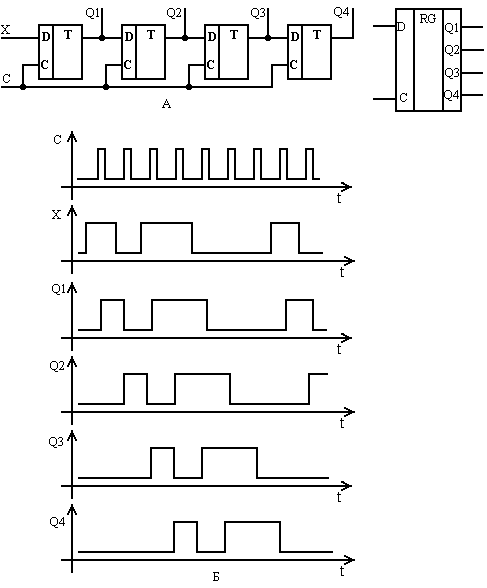
\includegraphics[width=0.6\textwidth]{14_register.png}
\caption{Регистр: схема реализации, УГО, схема сигналов}
\label{fig:14_register}
\end{figure}

\subsection*{Классификация регистров}

\begin{itemize}
\item накопительные;
\item сдвигающие. Которые в свою очередь делятся на:
	\begin{itemize}
	\item по способу ввода-вывода информации:
		\begin{itemize}
		\item параллельные
			\par запись и считывание информации происходит одновременно на все входы и со всех выходов
		\item последовательные
			\par запись и считывание информации происходит в первый триггер, а та информация, которая была в этом триггере, перезаписывается в следующий - то же самое происходит и с остальными триггерами
		\item комбинированные
		\end{itemize}
	\item по направлению передачи информации:
		\begin{itemize}
			\item однонаправленные
			\item реверсивные
		\end{itemize}
	\item по основанию системы счисления:
		\begin{itemize}
			\item двоичные
			\item троичные
			\item десятичные
		\end{itemize}
	\end{itemize}
\end{itemize}

Счётчик числа импульсов — устройство, на выходах которого получается двоичный (двоично-десятичный) код, определяемый числом поступивших импульсов. Счётчики могут строиться на двухступенчатых D-триггерах, T-триггерах и JK-триггерах.

Основной параметр счётчика — модуль счёта — максимальное число единичных сигналов, которое может быть сосчитано счётчиком. Счётчики обозначают через СТ (от англ. counter).

\subsection*{Классификация счетчиков}

\begin{itemize}
\item по числу устойчивых состояний триггеров
	\begin{itemize}
	\item на двоичных триггерах
	\item на троичных триггерах
	\item на n-ичных триггерах
	\end{itemize}
\item по модулю счёта:
	\begin{itemize}
	\item двоично-десятичные (декада)
	\item двоичные
	\item с произвольным постоянным модулем счёта
	\item с переменным модулем счёта
	\end{itemize}
\item по направлению счёта:
	\begin{itemize}
	\item суммирующие
	\item вычитающие
	\item реверсивные
	\end{itemize}
\item по способу формирования внутренних связей:
	\begin{itemize}
	\item с последовательным переносом
	\item с ускоренным переносом
		\begin{itemize}
		\item с параллельным ускоренным переносом
		\item со сквозным ускоренным переносом
		\end{itemize}
	\item с комбинированным переносом
	\item кольцевые
	\end{itemize}
\item по способу переключения триггера:
	\begin{itemize}
	\item синхронные
	\item асинхронные
	\end{itemize}
\item Счётчик Джонсона
	\par Счетчиком Джонсона называют кольцевой регистр, который строится на основе замкнутого регистра сдвига с одной перекрестной инверсной связью. Счетчик имеет коэффициент пересчета, вдвое больший числа составляющих его триггеров.
\end{itemize}


% Вопрос 15 ---------------------------------------------------------------------------------------------------------------
\section{Цифро-аналоговые преобразователи. Назначение. Принцип работы. Матрица R-2R. Область применения.}

Цифро-аналоговый преобразователь (ЦАП) — устройство для преобразования цифрового (обычно двоичного) кода в аналоговый сигнал (ток, напряжение или заряд). Цифро-аналоговые преобразователи являются интерфейсом между дискретным цифровым миром и аналоговыми сигналами.

Наиболее общие типы электронных ЦАП:

\begin{itemize}
\item Широтно-импульсный модулятор — простейший тип ЦАП. Стабильный источник тока или напряжения периодически включается на время, пропорциональное преобразуемому цифровому коду, далее полученная импульсная последовательность фильтруется аналоговым фильтром нижних частот. Такой способ часто используется для управления скоростью электромоторов, а также становится популярным в Hi-Fi-аудиотехнике;

\item ЦАП передискретизации, такие как дельта-сигма-ЦАП, основаны на изменяемой плотности импульсов. Передискретизация позволяет использовать ЦАП с меньшей разрядностью для достижения большей разрядности итогового преобразования; часто дельта-сигма ЦАП строится на основе простейшего однобитного ЦАП, который является практически линейным. На ЦАП малой разрядности поступает импульсный сигнал с модулированной плотностью импульсов (c постоянной длительностью импульса, но с изменяемой скважностью), создаваемый с использованием отрицательной обратной связи. Отрицательная обратная связь выступает в роли фильтра верхних частот для шума квантования.

\item Большинство ЦАП большой разрядности (более 16 бит) построены на этом принципе вследствие его высокой линейности и низкой стоимости. Быстродействие дельта-сигма ЦАП достигает сотни тысяч отсчетов в секунду, разрядность — до 24 бит. Для генерации сигнала с модулированной плотностью импульсов может быть использован простой дельта-сигма модулятор первого порядка или более высокого порядка как MASH (англ. Multi stage noise SHaping). С увеличением частоты передискретизации смягчаются требования, предъявляемые к выходному фильтру низких частот и улучшается подавление шума квантования;

\item ЦАП взвешивающего типа, в котором каждому биту преобразуемого двоичного кода соответствует резистор или источник тока, подключенный на общую точку суммирования. Сила тока источника (проводимость резистора) пропорциональна весу бита, которому он соответствует. Таким образом, все ненулевые биты кода суммируются с весом. Взвешивающий метод один из самых быстрых, но ему свойственна низкая точность из-за необходимости наличия набора множества различных прецизионных источников или резисторов и непостоянного импеданса. По этой причине взвешивающие ЦАП имеют разрядность не более восьми бит;

\item ЦАП лестничного типа (цепная R-2R-схема). В R-2R-ЦАП значения создаются в специальной схеме, состоящей из резисторов с сопротивлениями R и 2R, называемой матрицей постоянного импеданса, которая имеет два вида включения: прямое — матрица токов и инверсное — матрица напряжений. Применение одинаковых резисторов позволяет существенно улучшить точность по сравнению с обычным взвешивающим ЦАП, так как сравнительно просто изготовить набор прецизионных элементов с одинаковыми параметрами. ЦАП типа R-2R позволяют отодвинуть ограничения по разрядности. С лазерной подгонкой резисторов на одной подложке достигается точность 20-22 бита. Основное время на преобразование тратится в операционном усилителе, поэтому он должен иметь максимальное быстродействие. Быстродействие ЦАП единицы микросекунд и ниже (то есть наносекунды);
\end{itemize}

ЦАП находятся в начале аналогового тракта любой системы, поэтому параметры ЦАП во многом определяют параметры всей системы в целом. Далее перечислены наиболее важные характеристики ЦАП.

\begin{itemize}
\item Разрядность — количество различных уровней выходного сигнала, которые ЦАП может воспроизвести. Обычно задается в битах; количество бит есть логарифм по основанию 2 от количества уровней. Например, однобитный ЦАП способен воспроизвести два ($2^1$) уровня, а восьмибитный — 256 ($2^8$) уровней. Разрядность тесно связана с эффективной разрядностью (англ. ENOB, Effective Number of Bits), которая показывает реальное разрешение, достижимое на данном ЦАП.

\item Максимальная частота дискретизации — максимальная частота, на которой ЦАП может работать, выдавая на выходе корректный результат. В соответствии с теоремой Найквиста — Шеннона (известной также как теорема Котельникова), для корректного воспроизведения аналогового сигнала из цифровой формы необходимо, чтобы частота дискретизации была не менее, чем удвоенная максимальная частота в спектре сигнала. Например, для воспроизведения всего слышимого человеком звукового диапазона частот, спектр которого простирается до 20 кГц, необходимо, чтобы звуковой сигнал был дискретизован с частотой не менее 40 кГц. Стандарт Audio CD устанавливает частоту дискретизации звукового сигнала 44,1 кГц; для воспроизведения данного сигнала понадобится ЦАП, способный работать на этой частоте. В дешевых компьютерных звуковых картах частота дискретизации составляет 48 кГц. Сигналы, дискретизованные на других частотах, подвергаются передискретизации до 48 кГц, что частично ухудшает качество сигнала.

\item Монотонность — свойство ЦАП увеличивать аналоговый выходной сигнал при увеличении входного кода.

\item THD+N (суммарные гармонические искажения + шум) — мера искажений и шума вносимых в сигнал ЦАПом. Выражается в процентах мощности гармоник и шума в выходном сигнале. Важный параметр при малосигнальных применениях ЦАП.

\item Динамический диапазон — соотношение наибольшего и наименьшего сигналов, которые может воспроизвести ЦАП, выражается в децибелах. Данный параметр связан с разрядностью и шумовым порогом.

\item Статические характеристики:
	\begin{itemize}
	\item DNL (дифференциальная нелинейность) — характеризует, насколько приращение аналогового сигнала, полученное при увеличении кода на 1 младший значащий разряд (МЗР), отличается от правильного значения;
	\item INL (интегральная нелинейность) — характеризует, насколько передаточная характеристика ЦАП отличается от идеальной. Идеальная характеристика строго линейна; INL показывает, насколько напряжение на выходе ЦАП при заданном коде отстоит от линейной характеристики; выражается в МЗР;
	\item усиление;
	\item смещение.
	\end{itemize}

\item Частотные характеристики:
	\begin{itemize}
	\item SNDR (отношение сигнал/шум+искажения) — характеризует в децибелах отношение мощности выходного сигнала к суммарной мощности шума и гармонических искажений;
	\item HDi (коэффициент i-й гармоники) — характеризует отношение i-й гармоники к основной гармонике;
	\item THD (коэффициент гармонических искажений) — отношение суммарной мощности всех гармоник (кроме первой) к мощности первой гармоники.
	\end{itemize}
\end{itemize}

\begin{figure}[H]
\centering
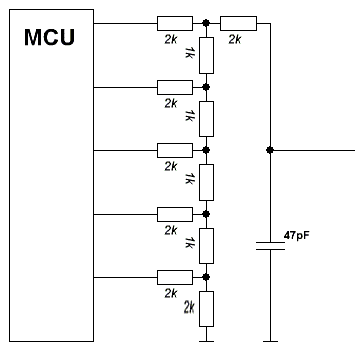
\includegraphics[width=0.5\textwidth]{15_R2R.png}
\caption{Схема R2R-матрицы}
\label{fig:15_R2R}
\end{figure}


% Вопрос 16 ---------------------------------------------------------------------------------------------------------------
\section{Аналого-цифровые преобразователи. Классификация. Область применения. Параллельные АЦП. АЦП поразрядного взвешивания.}

Аналого-цифровой преобразователь (АЦП, англ. Analog-to-digital converter, ADC) — устройство, преобразующее входной аналоговый сигнал в дискретный код (цифровой сигнал). Обратное преобразование осуществляется при помощи ЦАП (цифро-аналогового преобразователя, DAC).

Как правило, АЦП — электронное устройство, преобразующее напряжение в двоичный цифровой код. Тем не менее, некоторые неэлектронные устройства с цифровым выходом, следует также относить к АЦП, например, некоторые типы преобразователей угол-код. Простейшим одноразрядным двоичным АЦП является компаратор.

\begin{figure}[H]
\centering
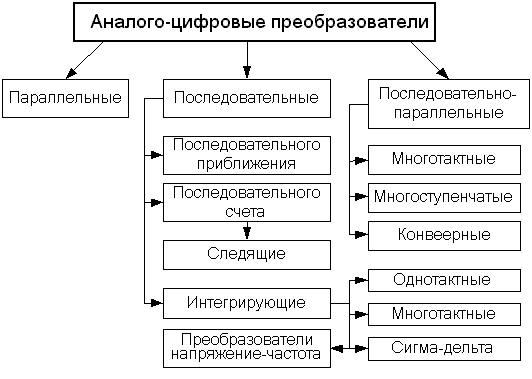
\includegraphics[width=0.7\textwidth]{16_ADC_scheme.png}
\caption{Классификация АЦП}
\label{fig:16_ADC_scheme}
\end{figure}

\subsection*{АЦП параллельного типа}
АЦП параллельного типа осуществляют квантование сигнала одновременно с помощью набора компараторов, включенных параллельно источнику входного сигнала. Ниже показана реализация параллельного метода АЦ-преобразования для 3-разрядного числа.

\begin{figure}[H]
\centering
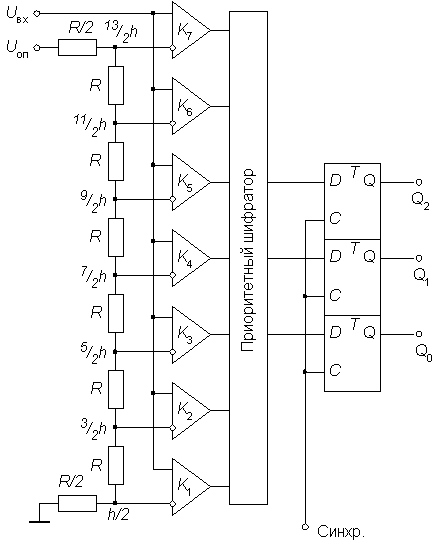
\includegraphics[width=0.6\textwidth]{16_parallel_ADC.png}
\caption{Устройство параллельного АЦП}
\label{fig:16_parallel_ADC}
\end{figure}

С помощью трех двоичных разрядов можно представить восемь различных чисел, включая нуль. Необходимо, следовательно, семь компараторов. Семь соответствующих эквидистантных опорных напряжений образуются с помощью резистивного делителя.

Параллельный АЦП является не только самым простым преобразователем с точки зрения операционной, но также и самым быстрым из всех типов АЦП, причём скорость работы ограничивается лишь задержкой на прохождение сигнала на логическом элементе и компараторе. К сожалению, в состав параллельных АЦП входит большое количество компонентов, причём размер схемы тем больше, чем выше разрядность АЦП. Для трёхразрядного АЦП требуются семь компараторов. В четырёхразрядной модели используется уже пятнадцать компараторов. По мере увеличения разрядности на одну единицу количество требуемых компараторов удваивается. Принимая в расчёт то, что восемь разрядов обычно считаются минимальным числом для обеспечения достаточной точности АЦП (то есть в случае параллельного АЦП необходимо 255 компараторов!), выявляется основная слабость технологии параллельных АЦП.

Другим, обычно не учитываемым, достоинством параллельных АЦП является возможность работы в нелинейном режиме. В случае использования в цепи делителя напряжения резисторов с равным номиналом каждый следующий импульс двоичного кода будет представлять одно и то же приращение аналогового сигнала, что будет обеспечивать пропорциональный выход. Однако в особых случаях в цепи делителя могут применяться резисторы с различными номиналами. Так образом реализуется нелинейный отклик на аналоговый входной сигнал. Никакой иной тип АЦП не позволяет обеспечить подобное преобразование сигнала путём простого изменением номиналов нескольких компонентов.

\subsection*{АЦП с поразрядным уравновешиванием}

АЦП с поразрядным уравновешиванием, является наиболее распространенным вариантом последовательных АЦП.

В основе работы этого класса преобразователей лежит принцип дихотомии, т.е последовательного сравнения измеряемой величины с 1/2, 1/4, 1/8 и т.д. от возможного максимального значения ее. Это позволяет для N-разрядного АЦП последовательного приближения выполнить весь процесс преобразования за N последовательных шагов (итераций) вместо $2^{N-1}$ при использовании последовательного счета и получить существенный выигрыш в быстродействии. Так, уже при N=10 этот выигрыш достигает 100 раз и позволяет получить с помощью таких АЦП до $10^5$...$10^6$ преобразований в секунду. В то же время статическая погрешность этого типа преобразователей, определяемая в основном используемым в нем ЦАП, может быть очень малой, что позволяет реализовать разрешающую способность до 18 двоичных разрядов при частоте выборок до 200 кГц (например, DSP101 фирмы Burr-Brown).

\begin{figure}[H]
\centering
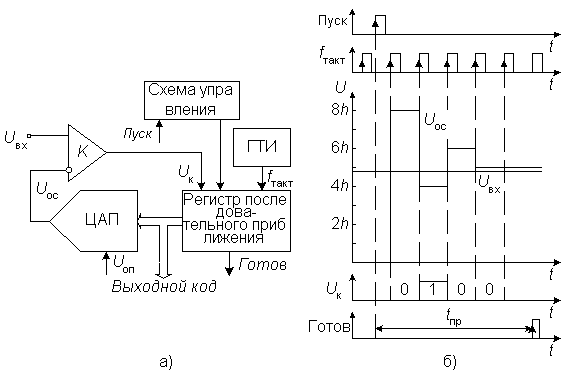
\includegraphics[width=0.8\textwidth]{16_ADC_serial_approx.png}
\caption{а) Устройство АЦП поразрядного взвешивания; б) Временная диаграмма}
\label{fig:16_ADC_serial_approx}
\end{figure}


% Вопрос 17 ---------------------------------------------------------------------------------------------------------------
\section{Интегрирующие АЦП. АЦП двойного интегрирования.}

\subsection*{Общие особенности}

АЦП данного типа осуществляют преобразование в два этапа.

\begin{enumerate}
\item На первом этапе входной аналоговый сигнал интегрируется и это проинтегрированное значение преобразуется в импульсную последовательность. Частота следования импульсов в этой последовательности или их длительность бывает промодулирована проинтегрированным значением входного сигнала.
\item На втором этапе эта последовательность импульсов преобразуется в цифровой код - измеряется ее частота или длительность импульсов.
\end{enumerate}

\subsection*{Общие достоинства}

\begin{enumerate}
\item АЦП данного типа нечувствительны к импульсным помехам.
\item АЦП данного типа нечувствительны к периодическим помехам если их период в целое число раз меньше периода интегрирования.
\item В результате, АЦП данного типа являются наиболее точными - типичная точность - 4...6 десятичных знаков, что соответствует 14...20 двоичным разрядам.
\item При работе АЦП данного типа в составе микропроцессорной системы возможна программная реализация части измерительной процедуры, а именно второго этапа - измерения временных характеристик последовательности импульсов, что упрощает преобразователь.
\end{enumerate}

\subsection*{Общие недостатки}

Преобразователи данного типа являются наименее быстродействующими из всех - типичное время преобразования - 1 - 1000 мс.

\subsection*{Программная реализация части преобразовательной процедуры}

Как уже отмечалось, при работе АЦП данного типа в составе микропроцессорной системы возможна программная реализация части измерительной процедуры, а именно второго этапа - измерения временных характеристик последовательности импульсов. Это измерение возможно как чисто программно при отсчете времени по счетчику команд или циклов, так и с использованием таймеров. В частности, для данных целей очень хорошо подходит устройство PCA, входящее в состав расширенных вариантов микроконтроллеров семейства MCS-51.

\subsection*{Классификация и примеры построения}

АЦП данного типа классифицируются, как правило, по типу преобразователя напряжение - импульная последовательность. Бывают преобразователи напряжение-частота (ПНЧ) либо - напряжение-время (ПНВ). Кроме того возможно построение преобразователей с постоянным тактом, циклом, зарядом или напряжением. Рассмотрим два варианта построения интегрирующих АЦП

\subsection*{АЦП с двойным интегрированием}

Это двухтактный преобразователь с заданной длительностью первого такта.

В течении первого такта происходит заряд интегрирующего конденсатора. Напряжение на нем в конце такта пропорционально интегралу входного напряжения.

Во время второго такта преобразования происходит разряд конденсатора заданным током до нулевого напряжения. Длительность этого такта и есть выходной сигнал преобразователя.

Достоинством данного варианта построения интегрирующего АЦП является не зависимость результата преобразователя от емкости интегрирующего конденсатора и пропорциональное изменение длительности второго такта при изменении длительности первого. Это позволяет снизить требования к точности тактовой частоты. В результате именно этот тип преобразователя используется в большинстве цифровых измерительных приборах.

\begin{figure}[H]
\centering
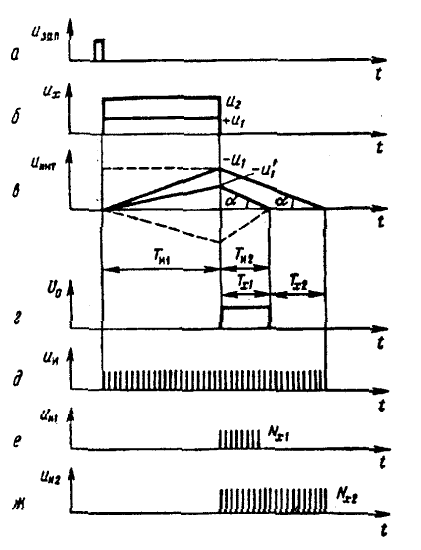
\includegraphics[width=0.5\textwidth]{17_ADC_2INT.png}
\caption{АЦП двойного интегрирования}
\label{fig:17_ADC_2INT}
\end{figure}


% Вопрос 18 ---------------------------------------------------------------------------------------------------------------
\section{Таймеры. Классификация. Область применения.}
% Вопрос 19 ---------------------------------------------------------------------------------------------------------------
\section{Источники вторичного напряжения. Структурные схемы. Выпрямители и фильтры.}

Вторичный источник электропитания — это устройство, предназначенное для обеспечения питания электроприбора электрической энергией, при соответствии требованиям её параметров: напряжения, тока, и т. д. путём преобразования энергии других источников питания. Согласно ГОСТ Р 52907-2008 слово «вторичный» опускается.

\subsection*{Классификация}

\begin{itemize}
\item Обеспечение передачи мощности — источник питания должен обеспечивать передачу заданной мощности с наименьшими потерями и соблюдением заданных характеристик на выходе без вреда для себя. Обычно мощность источника питания берут с некоторым запасом.
\item Преобразование формы напряжения — преобразование переменного напряжения в постоянное, и наоборот, а также преобразование частоты, формирование импульсов напряжения и т. д. Чаще всего необходимо преобразование переменного напряжения промышленной частоты в постоянное.
\item Преобразование величины напряжения — как повышение, так и понижение. Нередко необходим набор из нескольких напряжений различной величины для питания различных цепей.
\item Стабилизация — напряжение, ток и другие параметры на выходе источника питания должны лежать в определённых пределах, в зависимости от его назначения при влиянии большого количества дестабилизирующих факторов: изменения напряжения на входе, тока нагрузки и т. д. Чаще всего необходима стабилизация напряжения на нагрузке, однако иногда (например, для зарядки аккумуляторов) необходима стабилизация тока.
\item Защита — напряжение, или ток нагрузки в случае неисправности (например, короткого замыкания) каких-либо цепей может превысить допустимые пределы и вывести электроприбор, или сам источник питания из строя. Также во многих случаях требуется защита от прохождения тока по неправильному пути: например прохождения тока через землю при прикосновении человека или постороннего предмета к токоведущим частям.
\item Гальваническая развязка цепей — одна из мер защиты от протекания тока по неверному пути.
\item Регулировка — в процессе эксплуатации может потребоваться изменение каких-либо параметров для обеспечения правильной работы электроприбора.
\item Управление — может включать регулировку, включение/отключение каких-либо цепей, или источника питания в целом. Может быть как непосредственным (с помощью органов управления на корпусе устройства), так и дистанционным, а также программным (обеспечение включения/выключения, регулировка в заданное время или с наступлением каких-либо событий).
\item Контроль — отображение параметров на входе и на выходе источника питания, включения/выключения цепей, срабатывания защит. Также может быть непосредственным или дистанционным.
\end{itemize}

\subsection*{Трансформаторные ВИП}

Классическим блоком питания является трансформаторный БП. В общем случае он состоит из понижающего трансформатора или автотрансформатора, у которого первичная обмотка рассчитана на сетевое напряжение. Затем устанавливается выпрямитель, преобразующий переменное напряжение в постоянное (пульсирующее однонаправленное). В большинстве случаев выпрямитель состоит из одного диода (однополупериодный выпрямитель) или четырёх диодов, образующих диодный мост (двухполупериодный выпрямитель). Иногда используются и другие схемы, например, в выпрямителях с удвоением напряжения. После выпрямителя устанавливается фильтр, сглаживающий колебания (пульсации). Обычно он представляет собой просто конденсатор большой ёмкости.

Также в схеме могут быть установлены фильтры высокочастотных помех, всплесков (варисторы), защиты от КЗ, стабилизаторы напряжения и тока.

\begin{figure}[H]
\centering
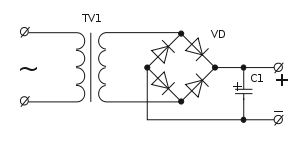
\includegraphics[width=0.8\textwidth]{19_transformer.png}
\caption{Схема простейшего трансформаторного ВИП}
\label{fig:19_transformer}
\end{figure}

\textbf{Структурная схема: трансформатор -> выпрямитель -> сглаживающий фильтр -> стабилизатор}

Достоинства трансформаторных БП:

\begin{itemize}
\item Простота конструкции.
\item Надёжность.
\item Доступность элементной базы.
\item Отсутствие создаваемых радиопомех (в отличие от импульсных, создающих помехи за счет гармонических составляющих).
\end{itemize}

Недостатки трансформаторных БП:

\begin{itemize}
\item Большой вес и габариты, пропорционально мощности.
\item Металлоёмкость.
\item Компромисс между снижением КПД и стабильностью выходного напряжения: для обеспечения стабильного напряжения требуется стабилизатор, вносящий дополнительные потери.
\item Слабая стойкость оборудования с таким БП к броскам напряжения и «отгоранию нуля» (обычно возникает в воздушных сетях сельской местности, приводит к повышению напряжения в розетках с 220 до 380 В). Печально известны в этом плане платы автоматики отопительных котлов (как правило они защищаются варистором, но часто и этого оказывается недостаточно). В то же время техника с импульсными БП (например, современные телевизоры) часто переносит повышения питания до 380 В без разрушения.
\end{itemize}

\subsection*{Импульсные ВИП}

Импульсные блоки питания являются инверторной системой. В импульсных блоках питания переменное входное напряжение сначала выпрямляется. Полученное постоянное напряжение преобразуется в прямоугольные импульсы повышенной частоты и определенной скважности, либо подаваемые на трансформатор (в случае импульсных БП с гальванической развязкой от питающей сети) или напрямую на выходной ФНЧ (в импульсных БП без гальванической развязки). В импульсных БП могут применяться малогабаритные трансформаторы — это объясняется тем, что с ростом частоты повышается эффективность работы трансформатора и уменьшаются требования к габаритам (сечению) сердечника, требуемым для передачи эквивалентной мощности. В большинстве случаев такой сердечник может быть выполнен из ферромагнитных материалов, в отличие от сердечников низкочастотных трансформаторов, для которых используется электротехническая сталь.

В импульсных блоках питания стабилизация напряжения обеспечивается посредством отрицательной обратной связи. Обратная связь позволяет поддерживать выходное напряжение на относительно постоянном уровне вне зависимости от колебаний входного напряжения и величины нагрузки. Обратную связь можно организовать разными способами. В случае импульсных источников с гальванической развязкой от питающей сети наиболее распространенными способами являются использование связи посредством одной из выходных обмоток трансформатора или при помощи оптрона. В зависимости от величины сигнала обратной связи (зависящему от выходного напряжения), изменяется скважность импульсов на выходе ШИМ-контроллера. Если развязка не требуется, то, как правило, используется простой резистивный делитель напряжения. Таким образом, блок питания поддерживает стабильное выходное напряжение.

\textbf{Структурная схема: выпрямитель -> фильтр -> генератор -> трансформатор -> выпрямитель -> фильтр -> стабилизатор}

Достоинства импульсных БП:

Сравнимые по выходной мощности с линейными стабилизаторами соответствующие им импульсные стабилизаторы обладают следующими основными достоинствами:

\begin{itemize}
\item меньшим весом за счёт того, что с повышением частоты можно использовать трансформаторы меньших размеров при той же передаваемой мощности. Масса линейных стабилизаторов складывается в основном из мощных тяжёлых низкочастотных силовых трансформаторов и мощных радиаторов силовых элементов, работающих в линейном режиме. Кроме того, благодаря повышенной частоте преобразования, значительно уменьшаются габариты фильтра выходного напряжения (можно использовать конденсаторы значительно меньшей ёмкости, чем для выпрямителей, работающих на промышленной частоте). Сам выпрямитель может быть выполнен по простейшей однополупериодной схеме, без риска увеличения пульсаций выходного напряжения;
\item значительно более высоким КПД (вплоть до 90-98 \%)[источник не указан 1182 дня] за счет того, что основные потери в импульсных стабилизаторах связаны с переходными процессами в моменты переключения ключевого элемента. Поскольку основную часть времени ключевые элементы находятся в одном из устойчивых состояний (то есть либо включен, либо выключен) потери энергии минимальны;
\item меньшей стоимостью, благодаря массовому выпуску унифицированной элементной базы и разработке ключевых транзисторов высокой мощности. Кроме этого следует отметить значительно более низкую стоимость импульсных трансформаторов при сравнимой передаваемой мощности, и возможность использования менее мощных силовых элементов, поскольку режим их работы ключевой;
\item сравнимой с линейными стабилизаторами надежностью. (Блоки питания вычислительной техники, оргтехники, бытовой электроники почти исключительно импульсные, линейные БП малой мощности сохранились только для питания слаботочных плат управления "белой"[неизвестный термин] бытовой техники вроде стиральных машин, микроволновых печей и отопительных котлов и колонок).
\item широким диапазоном питающего напряжения и частоты, недостижимым для сравнимого по цене линейного. На практике это означает возможность использования одного и того же импульсного БП для носимой цифровой электроники в разных странах мира — Россия/США/Англия, сильно отличных по напряжению и частоте в стандартных розетках.
\item наличием в большинстве современных БП встроенных цепей защиты от различных непредвиденных ситуаций, например от короткого замыкания и от отсутствия нагрузки на выходе.
\end{itemize}

Недостатки импульсных БП:

\begin{itemize}
\item Работа основной части схемы без гальванической развязки от сети, что, в частности, несколько затрудняет ремонт таких БП;
\item Все без исключения импульсные блоки питания являются источником высокочастотных помех, поскольку это связано с самим принципом их работы. Поэтому требуется предпринимать дополнительные меры помехоподавления, зачастую не позволяющие устранить помехи полностью. В связи с этим часто недопустимо применение импульсных БП для некоторых видов аппаратуры.
\item Как правило, импульсные блоки питания имеют ограничение на минимальную мощность нагрузки. Если мощность нагрузки ниже минимальной, блок питания либо не запускается, либо параметры выходных напряжений (величина, стабильность) могут не укладываться в допустимые отклонения.
\item В распределённых системах электропитания: эффект гармоник кратных трём. При наличии эффективно действующих корректоров фактора мощности и фильтров во входных цепях этот недостаток обычно не актуален.
\end{itemize}

\subsection*{Выпрямители}

Выпрямитель (электрического тока) — преобразователь электрической энергии; механическое, электровакуумное, полупроводниковое или другое устройство, предназначенное для преобразования переменного входного электрического тока в постоянный выходной электрический ток.

Большинство выпрямителей создаёт не постоянные, а пульсирующие однонаправленные напряжение и ток, для сглаживания пульсаций которых применяют фильтры.

\subsection*{Сглаживающий фильтр}

Сглаживающий фильтр — устройство для сглаживания пульсаций после выпрямления переменного тока диодным мостом. Простейшим сглаживающим фильтром является электролитический конденсатор большой ёмкости, установленный на схеме параллельно нагрузке, соблюдая полярность конденсатора. Нередко устанавливается параллельно электролитическому конденсатору плёночный (или керамический) для переменного тока ёмкостью 0,01 микрофарады, для устранения помех сети 220. Различают:

\begin{itemize}
\item Индуктивный
\item Ёмкостный
\item RC
\item LC
\end{itemize}


% Вопрос 20 ---------------------------------------------------------------------------------------------------------------
\section{Транзисторный усилительный каскад с общим эмиттером.}

Достоинства:

\begin{itemize}
\item Большой коэффициент усиления по току
\item Большой коэффициент усиления по напряжению
\item Наибольшее усиление мощности
\item Можно обойтись одним источником питания
\item Выходное переменное напряжение инвертируется относительно входного.
\end{itemize}

Недостатки:

\begin{itemize}
\item Худшие температурные и частотные свойства по сравнению со схемой с общей базой
\end{itemize}

Рассмотрим две простейшие схемы усилительных каскадов с общим эмиттером без температурной стабилизации рабочего режима в классе А с одним источником питания Eк.

\subsection*{Расчет в режиме покоя}

Все транзисторные каскады предварительного усиления, подобно аналогичным ламповым вариантам, работают в режиме класса А, при котором положение рабочей точки в режиме покоя (при Uвх = 0) выбирается на середине линейного участка динамической переходной характеристики. При этом постоянное напряжение смещения между базой и эмиттером Uбэ0 = const составляет доли вольта: (0,2 - 0,4) В для германиевых транзисторов и (0,4 - 0,7) В для кремниевых транзисторов, оно создается в режиме покоя в первой схеме (см. рис) фиксированным током базы Iоб = (Ек - Uбэ0) / Rб » Ек / Rб, проходящим в базовой цепи через входное сопротивление транзистора rвх тр-ра = rб + (1 + b) * rэ, резистор Rб » Ек / Iб0 и источник питания Ек.

\begin{figure}[H]
\centering
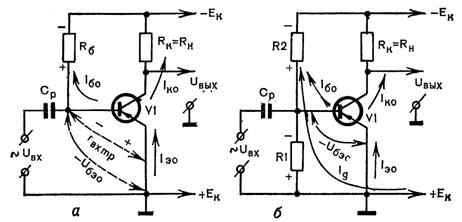
\includegraphics[width=0.7\textwidth]{20_schemes.jpg}
\caption{Две схемы транзисторных усилительных каскадов (а, б), работающих без температурной стабилизации, с одним источником питания в режиме класса А}
\label{fig:20_schemesmer}
\end{figure}

Во второй схеме усилительного каскада (см. рис) положение рабочей точки в режиме покоя фиксируется постоянным напряжением смещения Uбэ0 = Ек * R1 / (R1 + R2) с помощью делителя напряжения R1 и R2, через которые проходит ток делителя Iд=(2 - 5)*Iбо, создавая на R1 необходимую величину Uбэ0 = доли вольта.

Если в первой схеме на неизменность величины Uбэ0 влияет изменение Iб0 вследствие изменяющегося температурного режима, то во второй схеме величина тока делителя Iд не изменяется при колебании температуры.

Однако второй способ фиксации рабочей точки с делителем напряжения имеет недостаток, заключающийся в том, что для переменной составляющей входного тока уменьшается суммарная величина входного эквивалентного    сопротивления   каскада Rвх к-да = Rб || rвх тр-ра  так как Rб = R1 || R2, шунтируя входную цепь каскада, уменьшает его входное сопротивление. Это обстоятельство требует увеличения сопротивлений R1 и R2, вызывая нежелательное уменьшение необходимой величины тока делителя Iд, и соответственно уменьшая Iбо.

Учитывая это, на практике берут (R1 || R2) > rвх тр-ра. При этом

R1=Uбэ0/Iд, R2 = (Ек - Uбэ0)/(Iб0 + Iд).

Анализ работы транзисторного усилительного каскада осуществляется графоаналитическим методом, подобно ламповому варианту (рис 1.5.2).

На графике (см. рис) видно, что в режиме покоя при Uвх = 0, когда во входной базовой цепи течет базовый ток покоя Iб0 в выходной коллекторной цепи течет постоянный ток покоя коллектора Iк0 = (Ек - Uкэ0)/Rк, где Uкэ0 = Ек - Iк0 * Rк является нагрузочной линией по постоянному току, а сопротивление нагрузочного резистора в коллекторной цепи Rк = (Ек - Uкэ0)/Iк0, определяется графоаналитическим способом и выбирается такой величины, чтобы линия нагрузки проходила под углом a = arctg(1/Rк) ниже гиперболической кривой допустимой мощности, рассеиваемой на коллекторе транзистора Iк = Pк / Uк э.

Таким образом, нагрузочная линия будет построена в отрезках на осях координат по двум точкам. Первая точка в режиме холостого хода при Iк = 0, Uкэ = - Ек, а вторая точка в режиме короткого замыкания на выходе при Uкэ = 0; Iк = Ек / Rк.

\subsection*{Расчет в динамическом режиме}

В динамическом, т. е. рабочем, режиме усилительный каскад с общим эмиттером без температурной стабилизации работает следующим образом. При подаче входного сигнала uвх = Umвх*sinwt во входной цепи будет изменяться базовый ток iб = Iб0 + Imб * sinwt, вызывая изменение коллекторного тока iк = Iк0 + Imк * sinwt и соответствующее изменение выходного напряжения, снимаемое с коллектора и равное uвых = uкэ = Uкэо + Umкэ * sin(wt - p), отстающее по фазе от входного напряжения на 180 градусов.

\begin{figure}[H]
\centering
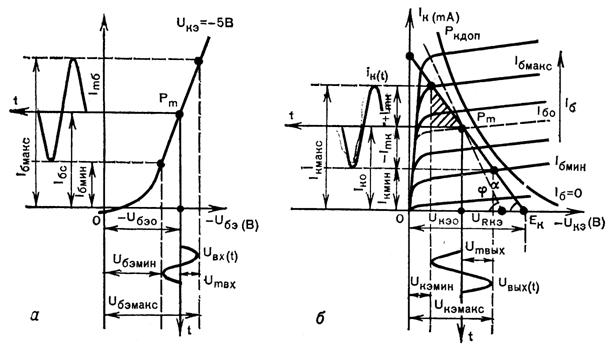
\includegraphics[width=0.8\textwidth]{20_analyze.jpg}
\caption{Графический анализ работы транзисторного усилительного каскада с ОЭ в классе А, с одним источником питания}
\label{fig:20_analize}
\end{figure}

Коэффициент усиления каскада при Rк = Rн без дополнительной внешней нагрузки и без учета влияния датчика входного сигнала ег и Rг

\begin{itemize}

\item по напряжению
\begin{equation}
K_U = -\dfrac{U_{out}}{U_{in}} = -\dfrac{\beta R_U}{R_{in\ cascade}}
\end{equation}

\item по току
\begin{equation}
K_I = \dfrac{\Delta I_K}{\Delta I_b} \approx \beta \approx h_{21e}
\end{equation}

\item по мощности
\begin{equation}
K_P = K_U * K_I
\end{equation}

\end{itemize}

Входное и выходное сопротивления каскада при указанных выше ограничениях и без учета малой величины емкостного сопротивления конденсатора, включенного во входную цепь каскада, можно определить по следующим формулам:

\begin{equation}
R_{in\ cascade} = U_{in} I_{in}
\end{equation}

\begin{equation}
R_{out\ cascade} = \dfrac{R_K}{1 + h_{22e} + R_K}
\end{equation}

так как дифференциальное сопротивление обратно смещенного коллекторного n-р-перехода rк >> Rк.

Полезная выходная мощность усиленного сигнала, выделяемая на резисторе Rк, будет равна:

\begin{equation}
P_\text{полезное} = P_{out} = I_K U_{KE} = \dfrac{I_{MK}U_{MKE}}{2} = 0,5 I^2_{MK}R_K
\end{equation}


% Вопрос 21 ---------------------------------------------------------------------------------------------------------------
\section{Дискретные цифровые САР: математическое описание, Z передаточные функции.}

Дискретными принято называть такие системы, в которых некоторые сигналы, передаваемые по каналам связи замкнутой системы, существуют только в отдельный момент времени или значение этих сигналов изменяется скачкообразно, ступенчато. Поэтому существует несколько типов дискретных систем, например, в которых производится квантование по уровню или по времени. % FIXME: картинка с квантованием

В цифровых системах управления квантование производится одновременно и по уровню и по времени. Значение сигнала существует в цифровой форме, соответствующей числу уровней в дискретные моменты времени. % FIXME: картинка с квантованием

\subsection*{Математическое описание дискретных систем}

Непрерывному сигналу x(t) в дискретных системах ставится в соответствие сигнал, соответствующий дискретному моменту времени:

\begin{equation}
x(t) = x(k\tau_r) \text{, где}
\end{equation}
\par $ k = 0, 1, 2, \ldots $;\nopagebreak
\par $ \tau_r $ --- период дискретизации.

Обычно дискретная система управления строится по следующему принципу:

\begin{figure}[H]
\centering
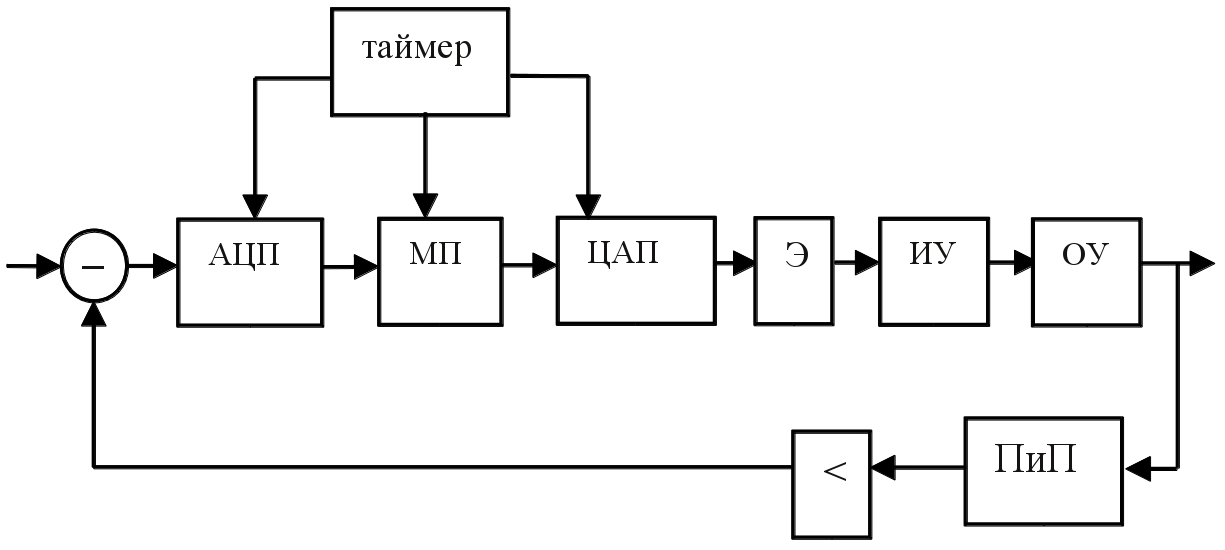
\includegraphics[width=0.7\linewidth]{21_dicret_struct.png}
\caption{Структура дискретной САУ}
\label{fig:21_dicret_struct}
\end{figure}

Это дискретная непрерывная система, в которой имеется аналоговый вход. А МП выступает в качестве цифрового регулятора. Таймер задает тактовые импульсы для процедур квантования по времени и выходных процедур. МП производит цифровую обработку сигнала в соответствии с законом регулирования. ЦАП преобразует число в последовательность импульсов, амплитуда которых может быть представлена ступенчато. Учитывая, что сигналы имеют малую мощность, то для управления эту мощность нужно усилить. Это делает экстраполятор --- заполняет промежуток между последующими импульсами по определенному закону. Простейший экстраполятор запоминает значение импульса на такт вперед. Он формирует ступенчатую огибающую последовательности импульса.

Дискретизация по времени приводит к тому, что система как замкнутая работает только в дискретные моменты времени. Поэтому упрощенная структура цифровых систем управления после линеаризации и структурных преобразований может быть представлена в виде совокупности линейной части и ключевого элемента:

\begin{figure}[H]
\centering
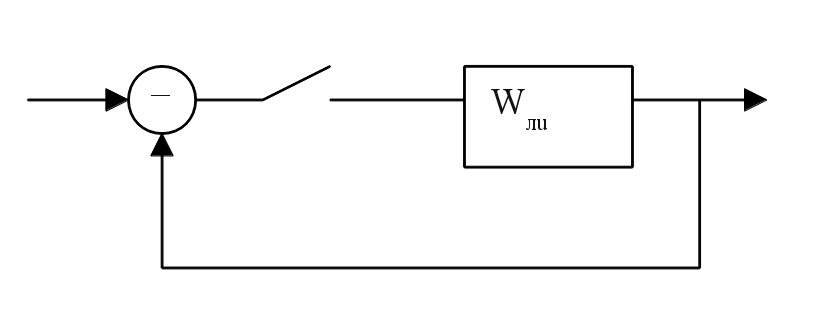
\includegraphics[width=0.5\linewidth]{21_dicret_struct_small.png}
\caption{Упрощённая структура дискретной САУ}
\label{fig:21_dicret_struct_small}
\end{figure}

Такое упрощение возможно благодаря высокому быстродействию современных вычислительных средств, то есть такая структура не учитывает запаздывания, создаваемого вычислительной процедурой.

Математическое представление дискретных систем сводится к представлению ДУ с помощью упрощенных процедур \textit{вычисления конечных разностей}.

Если в непрерывной системе вычисление первой производной представляется с помощью ДУ, то в дискретной системе $ \left( \dfrac{dx}{dt} \rightarrow \dfrac{\Delta^1x}{\tau_r} \right)  $  --- первая разность к периоду дискретизации:
\begin{equation}
\Delta^1x = x((k + 1)\tau_r) - x(k\tau_r).
\end{equation}

Для вычисления второй производной можно использовать равенство:

\begin{equation}
\left( \dfrac{d^2x}{dt^2} = \dfrac{\Delta^2x}{\tau^2_r} \right) \text{, где}
\end{equation}
\par $ \Delta^2x = \Delta^1((k + 1)\tau_r) - \Delta^1(k\tau_r) $;\nopagebreak
\par $ \Delta^2 = x((k + 1)\tau_r) - x((k + 1)\tau_r) - x((k + 1)\tau_r) + x(k\tau_r) $.

Используя процедуры численного интегрирования с использованием разностных процедур (например, на ЭВМ) можно получить следующее выражение, характеризующее дискретную САР:
\begin{equation}
y(k) = \sum_{i=0}^{m} x(k-m-i) - \sum_{j=0}^{n} y(k-n+i).
\end{equation}

Числа $y(k-n+i)$ и $x(k-m+j)$ характеризуют предыдущие значения выхода и входа ЦВМ, запоминаемые в памяти. Это уравнение называют \textit{рекурсивным или разностным}.

Реакция дискретной системы на дискретный сигнал так же может определяться с использованием принципа свертки функции:
\begin{equation}
y(k) = \sum_{k=0}^{n} x(k) w(k-n)\text{, где}
\end{equation}
\par $w(m)$ – весовая временная последовательность, аналог интеграла свертки.

Физический смысл: если на вход системы подается некий сигнал, который представлен в дискретной форме в момент времени $ k\tau $, будет соответствовать сумме реакций.

\subsection*{Z передаточные функции дискретных и цифровых САУ}

Z-преобразование получается путем замены переменных в дискретных преобразованиях Лапласа. Z-изображение дискретных сигналов дает возможность найти соотношение между z-изображением входных и выходных дискретных сигналов.

Z-преобразование содержит информацию о соответствующей непрерывной  функции времени только в дискретные моменты, поэтому оно определяет не непрерывную функцию, а ряд ее последовательных дискретных значений. Введение новой независимой переменной $ Z=e^{s\tau} $ позволяет перейти к рациональной функции:
\begin{equation}
Z[x^*\tau] = X(z) = \sum_{k=0}^{\infty} x(k\tau) Z^{-k}.
\end{equation}

Обратное Z-преобразование определяется формулой:
\begin{equation}
X^*(t) = Z^{-1} [X(z)] = \dfrac{1}{2\pi j} \oint\limits_r x(z) z^{k -1} dz
\end{equation}

Сигнал на выходе дискретных систем:
\begin{equation}
g(k) = \sum_{m=-s}^{\infty} w(k - m)g(m)\text{, где}
\end{equation}
\par $ w(k) $ --- весовая временная последовательной системы.

Отсюда:
\begin{equation}
W(z) = \dfrac{Y(z)}{G(z)}.
\end{equation}

Для непрерывной части дискретной системы Z-передаточная функция определяется на основе соотношения:
\begin{equation}
W(z) = \sum_{k=0}^{\infty} w(k\tau) z^{-k} \text{, где}
\end{equation}
\par $ w(k\tau) = [w(t)]_{t=k\tau} $;\nopagebreak
\par $ k = 1, 2, 3, \ldots $;
\par $ w(t) = L^{-1} [w(s)] $.

% Вопрос 22 ---------------------------------------------------------------------------------------------------------------
\section{Анализ дискретных САР.}

% Вопрос 23 ---------------------------------------------------------------------------------------------------------------
\section{Логарифмические частотные характеристики САР.}

% Вопрос 24 ---------------------------------------------------------------------------------------------------------------
\section{Переходные функции и переходные характеристики САР. Реакция САР на произвольный входной сигнал.}

% Вопрос 25 ---------------------------------------------------------------------------------------------------------------
\section{Типовые звенья САР и их частотные и временные характеристики.}

% Вопрос 26 ---------------------------------------------------------------------------------------------------------------
\section{Устойчивость линейных САР: определение, теоремы Ляпунова, алгебраический критерий устойчивости Гурвица.}

% Вопрос 27 ---------------------------------------------------------------------------------------------------------------
\section{Частотные критерии устойчивости линейных САР.}

% Вопрос 28 ---------------------------------------------------------------------------------------------------------------
\section{Анализ качества линейных САР.}

% Вопрос 29 ---------------------------------------------------------------------------------------------------------------
\section{Синтез корректирующих устройств линейных САР.}

% Вопрос 30 ---------------------------------------------------------------------------------------------------------------
\section{Анализ нелинейных САР.}

% Вопрос 31 ---------------------------------------------------------------------------------------------------------------
\section{Показатели качества ЭС.}

Показатели качества продукции --- количественная характеристика определенного свойства продукции на определенном этапе жизненного цикла.

Показатели качества продукции делятся на следующие группы:
\begin{enumerate}
\item Назначения
\item Надежности
\item Технологичности
\item Эргономические
\item Эстетические
\item Стандартизация и унификация
\item Патентно-правовые
\item Экономические
\end{enumerate}

Единичный показатель качества --- показатель качества продукции, относящийся только к одному из её свойств. Комплексный показатель качества --- показатель качества продукции, относящийся к нескольким её свойствам.

% Вопрос 32 ---------------------------------------------------------------------------------------------------------------
\section{Управление качеством ЭС.}

Управление качеством продукции базируется на статических методах контроля, зародилось в 30-е годы в связи с переходом к массовому производству изделий. В связи с этим стали применять выборочный контроль продукции с оценкой его результатов статистическим методом.
Контроль качества базируется на статистических методах и развиваясь циклически проходит через определенные этапы (см. рис)
\begin{center} 
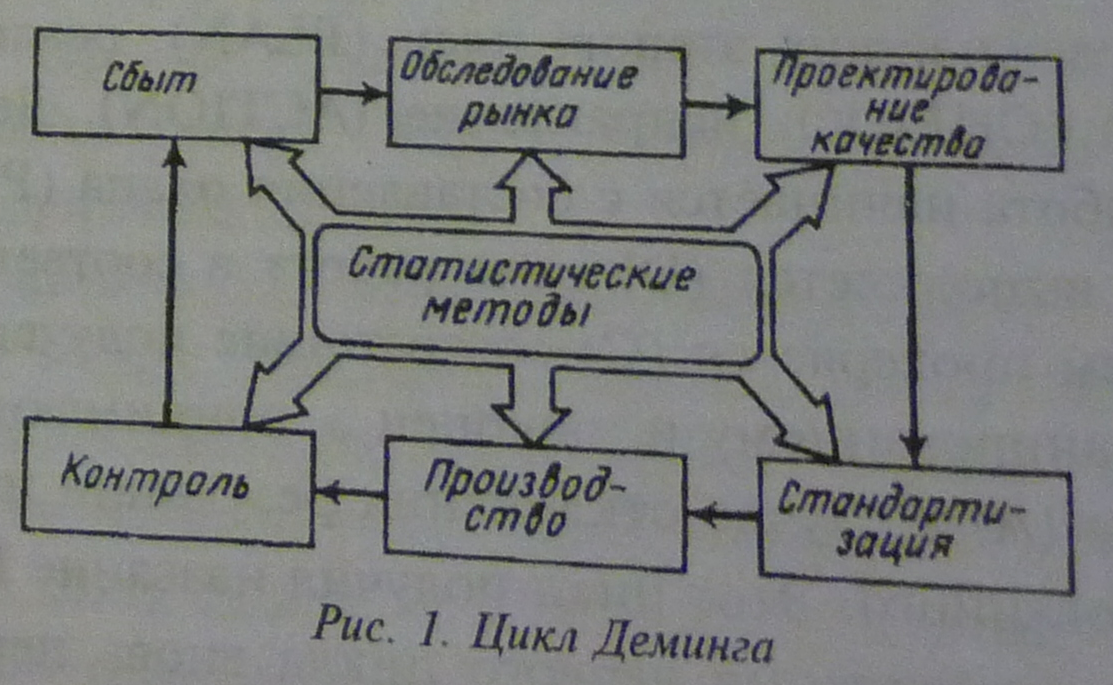
\includegraphics[width=0.6\textwidth]{32_Demming.png}\\
\end{center}

Управление качеством продукции базируется на статических методах контроля, зародилось в 30-е годы в связи с переходом к массовому производству изделий. В связи с этим стали применять выборочный контроль продукции с оценкой его результатов статистическим методом.

Контроль качества базируется на статистических методах и развиваясь циклически проходит через определенные этапы

Для эффективного обеспечения контроля качества необходимо участие всех, без исключения, работников предприятия. Такой контроль качества называется Тотальным(TQC). Был придуман и внедрен впервые в Японии 60х годах.

Среди статистических методов можно выделить 7 наиболее эффективных и доступных:
\begin{enumerate}
\item	Расслоение графики (полигон, гистограмма, кумулятивная кривая)
\item	Расслоение общей изменчивости статистических данных с помощью дисперсионного анализа.
\item	Диаграмма Парето
\item	Причинно-следственная диаграмма
\item	Диаграмма разброса (поле корреляции)
\item	Контрольная карта
\item	Контрольный лист
\end{enumerate}


% Вопрос 33 ---------------------------------------------------------------------------------------------------------------
\section{Себестоимость и уровень качества ЭС.}

Зависимость себестоимости и уровня качества продукции можно в общем виде представить в виде следующего графика (рис.)

СП – затраты на материалы, комплектующие  изделия, оборудование, заработную плату, контроль и испытания и т.д. 
 \begin{figure}
 \centering 
 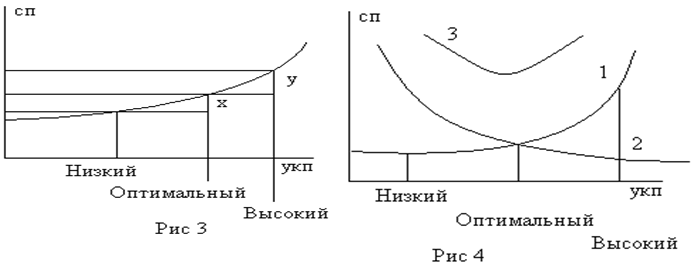
\includegraphics[width=0.7\textwidth]{33_Sebestoim.png}
 \caption{Слева -- зависимость себестоимости от уровня качества, справа --оптимальный уровень качества при затратах на изготовление и эксплуатацию.}
 \end{figure}
При повышении уровня качества от низкого до оптимального затраты растут медленно (х), поскольку производство легко справляется с заданными требованиями на уровень качества. По мере повышения УКП затраты (у) существенно возрастают. При дальнейшем повышении требований к УКП в конце концов достигается такой предел, когда ни оборудование, ни ТП, ни НТП и т.д. не в состоянии обеспечить требуемого (недостижимо высокого) качества. Затраты при этом устремляются в бесконечность.

Затраты на продукцию складываются из затрат на изготовление (проектирование и производство) и на эксплуатацию продукции (рис.).
Оптимальный уровень качества продукции - это такой уровень, выше или ниже которого производить продукцию экономически нецелесообразно.
При низком уровне качества продукции в сфере эксплуатации потребитель вынужден выделять дополнительные средства на ремонт, доработку и обслуживание продукции.
Высокий уровень качества продукции обуславливается ее высокой себестоимостью. 


\begin{enumerate}
\item Расслоение графики (полигон, гистограмма, кумулятивная кривая)
\item Расслоение общей изменчивости статистических данных с помощью дисперсионного анализа.
\item Диаграмма Парето
\item Причинно-следственная диаграмма
\item Диаграмма разброса (поле корреляции)
\item Контрольная карта
\item Контрольный лист
\end{enumerate}


% Вопрос 34 ---------------------------------------------------------------------------------------------------------------
\section{Корреляционная связь показателей ЭС.}

Диаграмма разброса применяется для исследования зависимости (корреляции) между двумя видами данных. Поэтому её часто называют полем корреляции.
С помощью диаграммы разброса удобно наблюдать процесс изменения параметра качества во времени при воздействии тех или иных факторов.

Совокупность точек на графике – диаграмма рассеяния.
С помощью диаграммы разброса можно определить имеется ли связь между параметрами и вид корреляции.(прямая корреляция, легкая прямая корреляция, обратная корреляция, легкая обратная корреляция, отсутствие корреляции, криволинейная корреляция.)

 \begin{figure}
 \centering 
 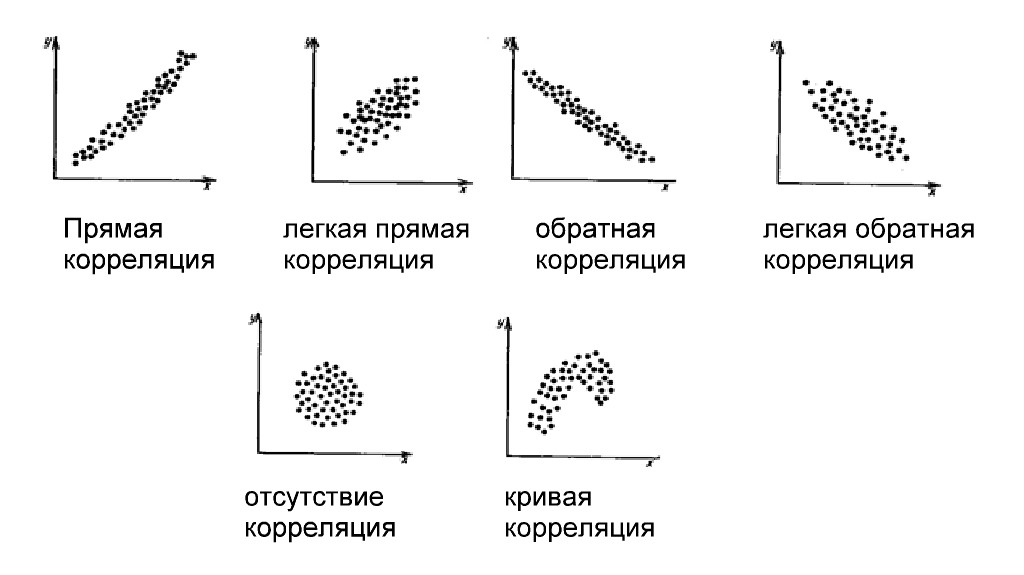
\includegraphics[width=0.8\textwidth]{34_Korelyacia2.JPG}
 \caption{Виды корреляции}
 \end{figure}
 
 Криволинейную корреляцию можно разделить на участки, имеющие прямолинейный характер, и исследовать каждый участок в отдельности.
 
 Степень связи может быть оценена: коэффициентом корреляции (прямолинейная), корреляционным отношением (криволинейная).
 
 Связь прямолинейную между Х и У можно найти:
 \begin{equation}
 Y-m_Y = r \cdot \frac{S_X}{S_Y} \cdot (X-m_Y),
 \end{equation}
 где r - коэффициент парной корреляции,
 \begin{equation}
 r = \frac{\sum_{i=1}^n (X_i - m_X)(Y_i-m_Y)}{(n-1) \cdot S_X \cdot S_Y},
 \end{equation} 
 \begin{equation}
 m_X = \dfrac{\sum_{i=1}^n X_i}{n}; S_X=\sqrt{\dfrac{\sum_{i=1}^n (X_i -m_X)^2}{n-1}},
 \end{equation}
 
  n - число пар наблюдений.
  
 $ -1 \leqslant r \leqslant 1$
 
 При |r|=1 – связь функциональная (зависимость между параметрами ввиде формул),
 
при |r|<1 – связь статическая. Каждому фиксированному значению Х соответствует ряд изменяющихся вместе с Х значений У и наоборот. Параметры Х и У считаются статистически зависимыми, если
\begin{center} 
  $\dfrac{\mid r \mid \cdot \sqrt{n-2}}{\sqrt{1-r^{2}}} \geqslant t_T = f(\alpha ; \nu = n-2)$\\
  \end{center}
  
Знак говорит о связи значений, если «-» то при уменьшении значения Х , У увеличивается и наоборот. Если «+» то при увеличении Х увеличивается и У.
  При r = 0 Х и У не связаны  между собой и не зависят друг от друга.

% Вопрос 35 ---------------------------------------------------------------------------------------------------------------
\section{Метод расслаивания <<4М>>.}

Простой и эффективный статистический метод, широко используемый в системе УК, - метод расслаивания

В основе метода – расслаивание статистических данных (т.е. группировка данных) в зависимости от условия их получения и обработка каждой группы в отдельности. Данные, разделённые на группы в соответствии с их особенностями, называют слоями (стратами), а сам процесс разделения на слои – расслаиванием (стратификацией). Существуют различные методы расслаивания, применение которых зависит от конечных задач. В производственных условиях обычно используется метод 4М, учитывающий факторы, зависящие от человека, машины, материала, метода. Расслаивание осуществляется:
\begin{enumerate}
\item по исполнителям – квалификации, полу, стажу работы и т.п.;
\item по оборудованию – году выпуска, марке, типу конструкции  и т.п.;
\item по материалу – месту производства, фирме-производителю и т.п.;
\item по способу производства 

\end{enumerate}

В результате расслаивания обязательно должны соблюдаться два условия:
\begin{itemize}
\item различия между значениями СВ внутри слоя должны быть как можно меньше по сравнению с различием её значений в не расслоенной исходной совокупности;
\item различие между слоями  должно быть как можно больше.
\end{itemize}	

При контроле качества изготовления изделий на практике возникает задача предполагаемого источника ухудшения качества продукции, когда разброс значений параметра качества около среднего значения возрастает. В случае нормального закона распределения контролируемого параметра качества такую информацию возможно получить путём расслаивания дисперсии с помощью дисперсионного анализа.

% Вопрос 36 ---------------------------------------------------------------------------------------------------------------
\section{Метод <<АВС-анализ>>.}

Метод служит для эффективности контроля качества изделия, для этого все изделия разбиваются по ценовым диапазонам (или иным критериям), составляется таблица,\\
\begin{center} 
  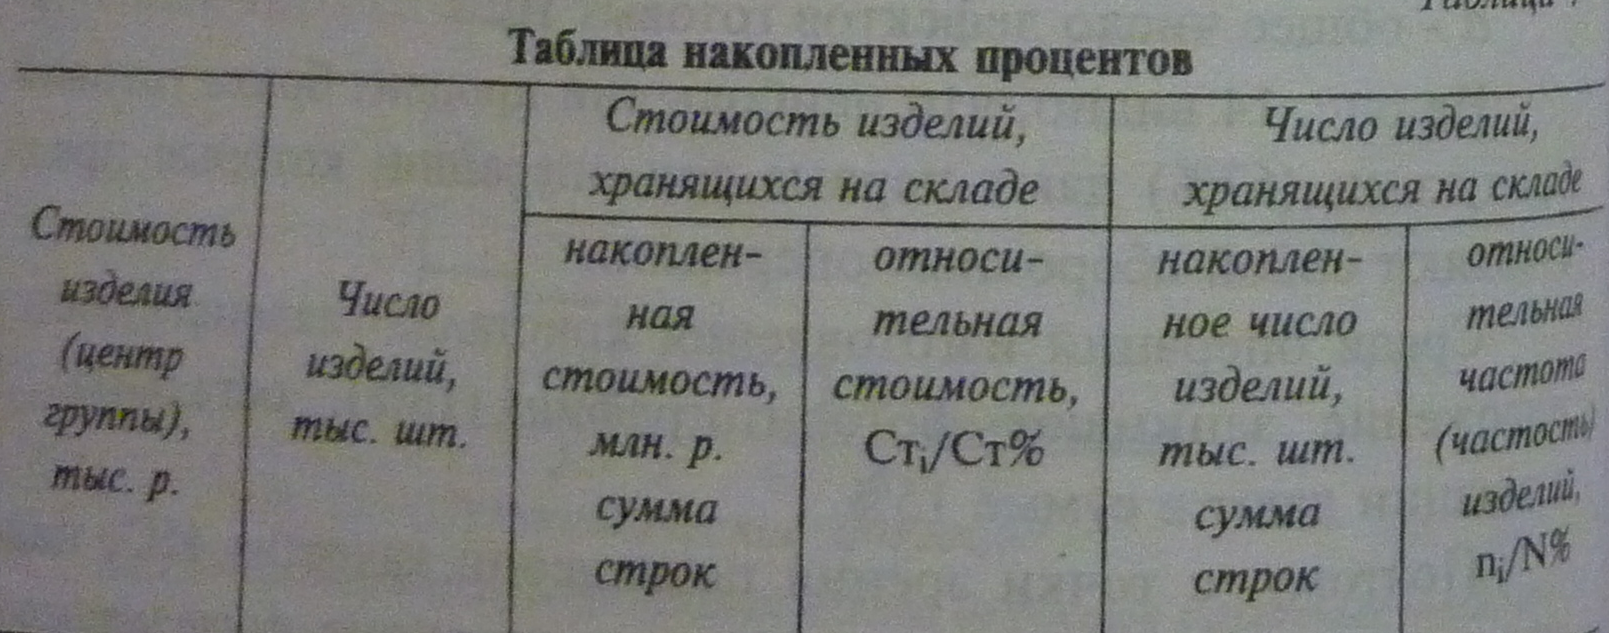
\includegraphics[width=0.7\textwidth]{36_Shapka.png}
  \end{center}
   и строится диаграмма Парето (по оси У откладывается относительная стоимость изделия в 
   \textdiscount
   , а по оси Х относительная частость изделий в
  \textdiscount). По результатам которой можно выделить три группы: группа А – наиболее дорогие изделия и её контроль должен быть наиболее строгим, группа С – наиболее дешевые изделия и её контроль упрощенный, все остальные изделия отнесутся к группе В и контроль качества должен быть средним.
  АВС-анализ широко применяется для контроля за производительностью труда, контроля денежных сумм, связанных со сбытом  и т.д.
  
\section{Виды статистического контроля ЭС.}
%Вопрос №37

Статистический контроль – это процесс установления соответствия между состоянием объекта и заданными на него нормами.\\
Контролем охватываются все этапы производства ЭС. В зависимости от стадии жизни изделия различают производственный и эксплуатационный контроль.

\underline{Производственный контроль} – (статический на стадии производства) охватывает все вспомогательные, подготовительные и технологические операции. В зависимости от места в цепи ТП произв контроль подразделяют на входной, операционный и приемочный.\\
\textit{Входной контроль} – контроль продукции поставщика. Материалы, комплектующие изделия подвергаются контролю на соответствие НТД.\\
\textit{Операционный контроль} – контроль продукции после завершения определенной операции.\\
\textit{Приемочный контроль} – контроль готовой продукции по окончании всех технологических операций.

\underline{Эксплуатационный контроль} – контроль, осуществляемый на стадии эксплуатации.\\
Часто статический контроль называют параметрическим контролем, потому что он базируется на контроле фактических значений параметров качества и сравнении их с запланированными значениями по НТД.

Перечисленные виды контроля могут быть как сплошными (100\textdiscount), так и выборочными.\\
Контроль по количественному признаку – регистрация точных числовых значений, измеряемых параметров качества.

Контроль по качественному признаку – выделяются категории к которым принадлежит контролируемое изделие. Частным случаем контроля по качественному признаку является контроль по альтернативному признаку – когда продукция разбивается на годную и не годную.
Летучий контроль – выборка из потока изделий в случайное время для контроля.

\section{Количественные показатели надежности ЭС.}
%Вопрос №38

Виды изделий:
	\begin{enumerate}
	\item По способу применения (изделия однократного и многократного действия);
\item	По способу обслуживания (восстанавливаемые и невосстанавливаемые изделия).
	\end{enumerate}
Восстанавливаемое ЭС -  изделие, изделия отказы которого устраняются путем ремонта (замены отказавшего элемента работоспособным). При этом само изделие состоит из невосстанавливаемых ЭРЭ (резисторов, конденсаторов, ИС) и узлов (собранных на гибридных и твердых схемах, микромодулях, микропроцессорах). Отказавшие ЭРЭ и узлы изымаются из изделия и заменяются на работоспособные.
Невосстанавливаемые являются изделия, не подлежащие ремонту в процессе эксплуатации.
\begin{itemize}
\item 	Показатели надежности  являются случайными величинами, т.к. все отказы случайные события
\item	Показатели надежности – функции времени.
	\end{itemize}
Показатели (их 5):
\begin{enumerate}


\item \underline{	Вероятность безотказной работы} p(t) – вероятность того что в заданном интервале времени (от 0 до t часов) в изделии не произойдет отказа.\\
p(t) = P(T>t), где Т – время безотказной работы, t – заданное время работы изделия.

Статистический расчет \\
\begin{equation}
p^{*}(t) = \frac{N(t)}{N_0} = \frac{N_0 - n(t)}{N_0} = 1- \frac{n(t)}{N_0}
\text{ где $N_0$ – общее число изделий, n(t) – число изделий отказавших за время t, N(t) – число изделий продолжающих работать после времени t.}\\
\end{equation}
$0 \leqslant p^{*}(t) \leqslant 1$.

Вероятность безотказной работы может быть и определена и для произвольного интервала времени (t1,t2). В этом случае говорят об условной вероятности безотказной работы
$P(t1,t2) = \frac{ P(t2)}{P(t1)}$
\item  \underline{	Вероятность отказа}q(t) - вероятность того что изделие откажет в течении заданного интервала времени (от 0 до t часов).
$q(t) = P(T \leqslant 1)$,
\begin{equation}
q(t) = 1-p(t),
\end{equation}
 вероятность отказа – противоположное событию безотказной работы.
 
Статистически значение находится по формуле\\
\begin{equation} q^{*}(t) = 1-p^{*}(t) = 1-1+\frac{n(t)}{N_0}=\frac{n(t)}{N_0},
\end{equation}
$0 \leqslant q^{*}(t)\leqslant 1$
\item	\underline{Частота отказов} f(t) – представляет безусловную плотность вероятности безотказной работы изделия. Она производная по времени от функции вероятности отказа\\
\begin{equation}f(t) = \frac{dq(t)}{dt} = -\frac{dp(t)}{dt} ,
\end{equation}
Частота отказа характеризует скорость изменения надежности (по вероятности безотказной работы) во времени, причем изменение происходит в сторону снижения надежности.

Статистически  она находится по формуле
\begin{equation}f^{*}(t) = \frac{n(t+\Delta t)-n(t)}{\Delta t \cdot N}= \frac{n(t)}{\Delta t \cdot N},
\end{equation} где $n(t+ \Delta t)$ – число отказавших изделий за время $ t+\Delta t$ \\
$f^{*}(t)$ – отношение числа отказавших изделий  в единицу времени t к общему числу изделий поставленных на испытания $N_0$.

\item \underline{Интенсивность отказов} $\lambda (t)$ – условная плотность вероятности безотказной работы.
\begin{equation} \lambda (t) = -  \frac{dp(t)}{dt} \cdot \frac{1}{p(t)} =  \frac{f(t)}{p(t)},
\end{equation}

Статистически интенсивность находят как\\
\begin{equation} \lambda^{*}(t)=\frac {f^{*}(t)}{p^{*}(t)}=\frac{n(\Delta t)}{\Delta t \cdot N(t)}
\end{equation}

Графическая зависимость интенсивности отказов от времени для большинства ЭС имеет вид\\
\begin{figure}[H]
\centering
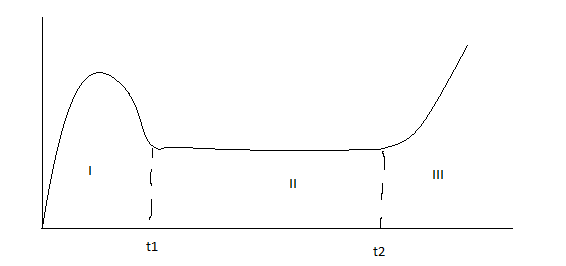
\includegraphics[width=0.6\textwidth]{38_Zhizn2.png}
\caption{Зависимость интенсивности отказов ЭС от времени: I - 0-t1 период приработки изделия, II - t1-t2 период эксплуатации изделия, III - t2-$\infty$ период старения и износа изделия}
\label{fig:Zhizn}
\end{figure}
В 1 периоде отказы ЭРЭ, узлов  происходят из-за: некачественного монтажа, сборки, низкой надежности элементов, контактов , проводников.
Во 2 периоде число отказов стабилизируется , но оно не равно нулю.
В 3 периоде отказы изделия происходят из-за физического старения материалов и износа ЭРЭ, имеющие необратимый характер.
Для нахождения р(t) = F[$\lambda$(t)] проинтегрируем $\lambda(t)$,
\begin{equation}\int_0^t \lambda (t) =- \int_0^t \frac{dp(t)}{dt} \cdot \frac{1}{p(t)} ,
\end{equation}
\begin{equation} -\int_0^t \lambda (t)dt = \int_0^t \frac{dp(t)}{p(t)}, -\int_0^t \lambda (t)dt = \ln p(t) ,
\end{equation}
\begin{equation}
p(t) = e^{- \int_{0}^{t} \lambda(t)dt}
\end{equation}

Вероятность безотказной работы имеет экспоненциальный вид, аналогично может быть найдена условная вероятность безотказной работы за интервал времени (t1,t2)
\item \underline{	Средняя наработка до отказа}
Tcp(t) – время работы изделия до первого отказа.
\begin{equation}
T_{cp} (t)= \int_0^\infty p(t)dt,
\end{equation}
Статистически оно находится
\begin{equation}
T^{*}_{cp} (t) = \frac{1}{N_0} \sum_{i=1}^{N_0} t_i,
\end{equation}
где $t_i$ – время работы до отказа i-го однотипного изделия.
Рассмотрим расчет показателей надежности ЭС для 2 периода $ \lambda(t)=const = \lambda$
\begin{equation}
p(t)= e^{- \lambda t},
\end{equation}
\begin{equation}
T_{cp}(t) = \int_0^\infty p(t)dt= \int_0^\infty e^{- \lambda t}dt = \frac{1}{\lambda},
\end{equation}
Рассмотренные показатели надежности справедливы для невосстанавливаемых ЭС.
\end{enumerate}

\section{Последовательная модель надежности ЭС.}
%Вопрос №39

При последовательном соединении элементов расчет надежности производят по формуле %formula

 \begin{equation}
 P_A(t) = {\prod_{i=1}^{m}p_i(t) }
 \end{equation}
Для большего значения вероятности безотказной работы каждый элемент должен иметь значение вероятности безотказной работы близкой к единице.\\
$P_A(t)\leqslant1$,
 при увеличении количества компонентов в ЭС надежность его падает.(пример)
В тех случаях , когда нужна высокая надежность ЭС, а элементы имеют небольшое значения вероятности безотказной работы, применяют метод резервирования.

\section{Параллельная модель надежности ЭС.}
%Вопрос №40

При параллельном соединении элементов расчет надежности производят по формуле 
 \begin{equation}
 P_A(t) = {1- \prod_{i=1}^{m}[1-p_i(t)] }
 \end{equation}
% Вопрос 41 --------------------------------------------------------
\section{Основные этапы автоматизации:  их характеристики и особенности}

\underline{Этапы развития автоматизации}\\
\textit{Первый этап} - автоматизация цикла обработки с целью получения заданной формы, размеров и качества обрабатываемой поверхности, цикла сборки для фиксации сборочного соединения.

Средства автоматизации - ЧПУ обеспечивающие эффективное использование технологического оборудования только в крупносерийном и массовом производстве.

\textit{Второй этап} - наряду с автоматизацией цикла обработки (сборки) обеспечивается автоматизация загрузки и разгрузки основного технологического оборудования. Такое оборудование оснащено магазинами заготовок и готовых деталей в виде комплектов под сборку и загрузочными устройствами, приспособленными в обслуживанию определенной номенклатуре деталей, функции загрузки-разгрузки может выполнять ПР, установленный совместно с ЧПУ, который обеспечивает возможность использования оборудования в серийном производстве.

\textit{Третий этап} - предусматривает автоматизацию контроля за ходом выполнения техпроцесса и его оптимизацию. При этом выделяется 2 вида контроля:
\begin{itemize}
    \item проверки соответствия заготовок (комплектующих деталей при сборке), инструмента, состояния технологического оборудования установленным характеристикам с целью внесения коррекции настройкой оборудования или удаления из потока некондиционных деталей.
    \item проверка текущего состояния инструмента и оборудования путем измерения силовых, температурных деформаций и сравнения текущих параметров с эталонными.
\end{itemize}

Таким образом, учитывается влияние случайных и систематических факторов на характер тех. процесса.

\textit{Четвертый этап }- обеспечивается автоматизация переналадки оборудования на обработку (сборку) объектов производства другого назначения. Это возможно при использовании, к примеру, обрабатывающих и сборочных центров, оснащенными ПР с наборами сменных инструментов, захватных устройств, системы накопителей под номенклатуру обрабатываемых или собираемых узлов (деталей) и оснастки. В этом случае размер изготовляемой партии изделий не имеет значения, ограничивающего гибкость робототехнического производства, классификация (признаки классификации).

% Вопрос 42 --------------------------------------------------------
\section{Назначение, классификация и области применения роботов}

Можно разделить на 3 класса:
\begin{enumerate}
\item	манипуляционные или роботы манипуляторы;
\item	информационные;
\item шагающие
\begin{itemize}

\item  роботы-экзоскелеты (медицинские, роботы-усилители);
\item шагающие аппараты.
\end{itemize}
\end{enumerate}
Манипуляционные: 
\begin{enumerate}
\item	промышленные (универсальные, специальные, специализированные);
\item погрузочные манипуляторы;
\item	для экстремальных сред (космические, подводные, для радиоактивных сред, для токсичных сред, взрывобезопасные);
\item	медицинские;
\item	бытовые;
\end{enumerate}
Наиболее обширен класс роботов-манипуляторов.

Класс информационных роботов включает в себя аппараты для исследования космического пространства,подводного дна и т.п. Они предназначены для автоматического получения и передачи информации об исследуемых объектах.

Класс шагающих роботов включает в себя а), кто предназначены для восстановления двигательных функций человека или для технического усиления мощности двигательных конечностей здорового человека (б).

% Вопрос 43 --------------------------------------------------------
\section{Манипуляционные роботы: типы, характеристики, применение}

Они представляют собой техническую систему, заменяющую труд человека, в состав которого входят орган воздействия на окружающую среду, т.е манипуляционные устройства или манипулятор-это исполнит. Орган, имитирующий действие человеческой руки в достаточно широком диапазоне масштабов увеличения или уменьшения ее геометрических размеров и мощности.

Обобщенная функц. схема манипуляционного робота имеет следующий вид:
\begin{figure}
\centering
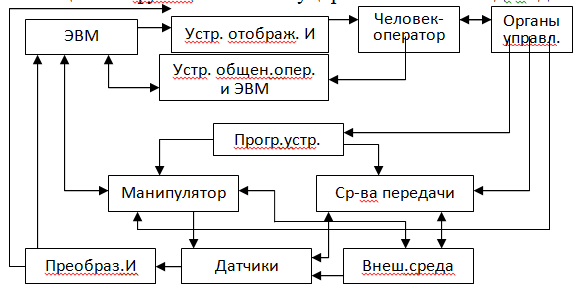
\includegraphics[width=0.8\textwidth]{44_Manipul_robot.png}
\caption{Обобщенная функциональная схема манипуляционного робота}
\end{figure}

Различные группы манипуляц. роботов включают в себя ту или иную часть блоков и связей, составляющих обобщенную схему.

Манипуляц. робот м. иметь 1 или несколько манипуляторов. Движения манип-ров м. отличаться от движения руки ч/а. В суставах, звеньях манип-ров м. не только вращаться, но и перемещаться поступательно. М. изменяться длина некоторых звеньев. Кисть руки имитируется с пом. захвата (м.б. 2-хполый, 3-хпалый или более). На захвате м.б. установлены различные датчики.

Средства передвижения м.б. колесными, гусеничными, шагающими, плавающими и т.д.
Устанавливаемые датчики И. позволяют роботу ориентироваться во внешней среде.
По способу упр-я манипуляц. роботов разделяют на 3 группы: автоматич.,биотехнические, комбинированным управлением.

\textit{Автоматическими} манипуляц. роботами называют  устройства, ктр. действуют без непосредственного участия ч/а в упр-ии. Они прим-ся в тех случаях, когда манипуляц. устр-во удалено на значит. расст. от органов упр-я, либо когда очень высокий темп работ, опасны внешняя среда или объект действия, а ручное упр-е нецелесообразно.
Выделяют: I покол.(программн, интеллектуальные, адаптивные).

\textit{Биотехнич.} манипуляц. роботы – робот, в систему упр-я ктр-х включен человек-оператор. М.б.: командные – упр-ся оператором дистанционно с командного устр-ва с нажатием кнопок или с помощью упр-щей рукоятки.

\textit{Копирующие} манипуляц. роботы имеют задающий орган, геометрически подобный манипуляц-ому устр-ву. При этом способе упр-я привод каждого звена вместе с соответствующим датчиком образует дистанционно следящую систему. Если положения задающего органа и манипуляц. устр-ва совпадают, то последнее стремится к 0 ошибке по положению.

% Вопрос 44 --------------------------------------------------------
\section{Структура механизмов манипуляционных роботов и характеристики их геометрических свойств}

Механизмом называют механич. систему, предназначенную для получения требуемого движения 1-го или нескольких тел.

Основными элементами являются: звенья и кинематич. пары.

Звено-1 или неск жестко соединенных твердых тел, входящих в состав механизмов.
Звенья:
\begin{enumerate}
\item простые состоят из 1-го твердого тела;
\item составные – из нескольких твердых дел.
\end{enumerate}

Кинематич. пара – соединение двух смежных звеньев, допусккающие их относит. движение. Звенья м. соприкасаться пов-тями, линиями и точками.
Кинематич. пара м.б. плоской, если относит. движение сочлененных звеньев возможно лишь в параллельных плоскостях или в пространстве, если относительное движение сочлененных звеньев возможно в любом направлении.

С целью уменьшения потерь и увеличения износостойкости между звеньями вводят промежуточные элементы (ролики или шарикоподшипники). Такие совокупности образуют кинематич. соединение.

Кинематич. пары классифицируются по числу условий связи на относительное движение двух смежных тел или по числу степеней свободы. Каждое условие связи кинематич. пары не только устраняет относительную подвижность, но и позволяет передавать от звеньев к звеньям силовое воздействие.

Свободное тело в пространстве имеет 6 степеней своб:3 поступательные движения в направлении оси x,y,z, 3 вращательных движения относительно этих осей.

Если 1 звено превратить в стойку, то для 2-го звена в соответствии с конструкцией кинематич. пары: W=G-U, U-число связей, налагаемых кинематич. парой на относительно движения ее звеньев. При U=0 пара отсутствует, т.к. отсутствуют связи между звеньями. При U=6 относительного движения звеньев нет, т.к. они образуют 1 звено. Поэтому число условий связи кинематич. пар м. находиться в пределах от 1 до 5. Соответственно этому все кинематич. пары делят на 5 классов или на 5 родов по числу степеней свободы.

Кинематич. пары 1 и 2 классов в манипуляц-х роботах не применяются. Примеры кинематич. пар манипуляц. устр-в:
Класс 3, род 3 – 3 степени свободы, класс 4, род 2 – 2 степени свободы.

Кинематич. пара 3 класса 3 рода предст. собой шаровой шарнир , имеющий 3 степени свободы-вращение относительно каждой из осей.

 Кинем. пара 4 класса 2 рода м.б. реализована либо вращением одной из осей, указанных в системе коорд. и поступат. движ. Вдоль 1 оси, либо вращениие относит. двух взаимоперпендикулярных осей.

Кин. пара 5 класса 1 рода позволяет иметь лишь одно относит. движение-либо вращение, либо поступат. движение вдоль 1 оси.

Кинемат. цепью называют связанную систему звеньев, образующих кинематич. пару. Они бывают замкнутыми и открытыми. Замкнутая кинемат.цепь – такая цепь, в ктр.звенья входят не менее, чем в 2 кинемат. пары. Открытая кинем. цепь – цепь, в ктр. имеются отдельные звенья, входящие только в 1 кинем. пару.

Механизм манипуляц. робота представляет собой сложную открытую кинем. цепь, у ктр-х 1 звено обращено в стойку, а движение вых-х звеньев вполне опр-ся заданным движением входных звеньев.

Манипуляц. устр-ва предст. собой открытую кинематич. цепь, в ктр. число n подвижных звеньев всегда = числу кинематич. пар. Тогда число степеней свободы для механизма манипуляц-го устр-ва опр-ся как: \begin{equation}
W=3p3+2p4+p5
\end{equation}
\begin{equation}
n=p3+p4+p5
\end{equation}

Пространств. исполнит. механизмы м. иметь большое число степеней свободы во многих отношениях они аналогичны руке человека. Однако число звеньев чел. руки достаточно велико (n=19) и число степеней свободы W=27. В наст. время ни один механизм не обладает такими возм-тями . Однако при существующем уровне техники-это не так уже важно.

Характеристики геом-х св-в манип-х устр-в:
\begin{enumerate}
\item  \underline{Зона обслуживания}

У манипуляц-х устр-в выделяют базовую плоскость, плоскость ктр образована плечом и предплечием мнипулятора и в ктр м. располагаться одновременно оси всех его звеньев.

Зоной обслуживания манипуляц-го робота называют сов-ть точек базовой плоскости, ктр. м. достигать захват манипуляц-го устр-ва. Преимущественное распространение получили манипуляторы с упорядоч-м расположением звеньев кинематич-х пар , т.е. такие, когда имеется 1 пара смежных кинематически связанных звеньев, ктр обеспечивает перенос кисти в базовой плоскости в любую точку зоны обслуживания.

\item \underline{Рабочий объем} или рабочие зоны манипуляц-го устр-ва называют пространство , ограниченное поверхностью, огибающей все возможные положения захвата. Для обеспечения наиболее полного обслуживания любой точки необходим механизм манип-ра, исп-щий не менее 6 степеней свободы, из ктр-х 3-для перемещения кисти, 3-для ориентации захвата кисти. Тогда в зависимости от сочетания кинем. пар, обеспечивающих перемещения кисти различают 3 осн.формы рабочего объема:
\begin{itemize}
\item	прямоугольный, когда кисть пеермещается в пространстве с пом. Механизма с 3-мя поступат-ми кинем-ми парами 5 класса;
\item цилиндрич., когда исп-ся механизм с двумя поступательными и 1 вращательной кинем.парой;
\item сферический, когда исп-ся 2 вращат. и 1 поступат., либо 3 вращат. кинематич. пары.
\end{itemize}
\item  \underline{Движение манипуляц. робота} и его манипуляц-го устр-ва. Для манипуляц-х роботов вводят понятие глобальных, региональных и локальных движений.

К глобальным движениям робота относят его перемещ-я в пространстве с пом. средств передвижения.
Регион.движения робота-это движения по переносу кисти его манипуляц-го устр-ва в любую точку рабочего объема.

Локальные движения робота связаны с ориентацией кисти в пространстве и движение по захвату объектов действий, движение манипулятора в его рабочем объеме м. классифицировать:
\begin{itemize}
\item	Движение манипуляц-го устр-ва, несущего своб. объект и совершаемые в своб. объеме
\item	Целенаправленное движение манипуляц-го устр-ва по перемещению своб-го объекта, совершаемые в несвободном рабочем объеме
\item	Движение манипуляц-го устр-ва в своб. объеме, согласованные с движением объекта действия
\item	Движения манипуляц-х устр-в в несвоб.объеме, согласованные с перемещением объекта действий.
\end{itemize}
\item \underline{Маневренность}

Ключевой А и запястный кистевой механизм С имеют каждый 3 степени  свободы. Они позволяют ориентировать кисть 3 на нектр. Участки поверхности сферы с радиусом, равным пределе сумм длин плеча 1 и 2.
Кинематич.пара 5 класса в локтевом суставе В позволяет менять радиус сферы и доставлять захват в любую точку сферического рабочего объема.
Если зафиксировать захват 4 неподвижные точки. Манип. устр-во будет иметь возможность совершать круговое движение плечами 1 и 2. Т.о. св-ва манип-го устр-ва м. иметь подвижность при фиксированном захвате называется маневренностью. В рассм-вом случае механизм сохраняет 1 степень свободы, что оперделяет степень маневренности манип. устр-ва.

Повышение числа степеней маневренности позволяет выполнять движения более сложных классов, сужает мертвые зоны манип-го устр-ва и увеличивает свободу действий оператора.

Перестановка кинем. пар в данном устр-ве, н-р, А вместо В не меняет число степеней свободы, но при фиксированном захвате превращение манипуляц. устр-во в ферму и механиизм теряет свою маневренность.
\end{enumerate}

% Вопрос 45 --------------------------------------------------------
\section{Приводы манипуляторов и роботов: классификация, особенности применения}

В зависимости от используемого вида энергии приводы подразделяют на гидравлические, пневматические, электрические и комбинированные (например, электрогидравлические, гидропневматические и др.) Часто их применяют в комбинации, например, в звеньях манипулятора большой грузоподъемности используют гидравлический привод, а в его захватном устройстве — более простой и маломощный пневматический.

\underline{Пневматические} приводы применяются в 20…30\textdiscount (по другим оценкам в 40-50\textdiscount) серийно выпускаемых ПР. Их используют  для легких и средних (по грузоподъемности до 20 кг) ПР при числе степеней подвижности 2…3. Погрешность позиционирования в этих приводах не превышает ± 0,1 мм. Скорость ведомого звена привода при линейном перемещении составляет до 1000 мм/с, при угловом – до 60 об/мин. Они имеют простую конструкцию, низкую стоимость и достаточно надежны в работе.

Вследствие низкой регулировочной способности их мало используют в позиционных и контурных режимах работы, и они имеют цикловое управление, как простейший вариант позиционного (задается две точки – начало и конец перемещения).

\underline{Гидравлические} приводы применяются в 30\textdiscount серийно выпускаемых средних и тяжелых ПР при числе степеней подвижности 3…4. Погрешность позиционирования в этих приводах не превышает ± 0,5 мм при скорости линейного перемещения до 0,8…1200 мм/с. Эти приводы имеют сложную конструкцию, высокую стоимость изготовления и эксплуатации. Гидравлический привод имеет хорошую регулировочную способность, и его используют в ПР с позиционным и контурным режимом работы.

\underline{Электрические} приводы используются в 40…50\textdiscount серийно выпускаемых ПР со средней грузоподъемностью и числом степеней подвижности 3…6. Точность позиционирования электрического привода достигает значений до ± 0,05 мм. Их применяют как в позиционном, так и в контурном режимах работы. 

Преимуществами электроприводов являются более высокая экономичность, КПД, удобство сборки и хорошие регулировочные свойства. 

Как правило, в электроприводах используют синхронные, шаговые и двигатели постоянного тока. Асинхронные двигатели применяются реже, что связано с трудоемкостью управления частотой вращения.

\underline{Комбинированные} приводы позволяют максимально использовать достоинства отдельных типов приводов. Чаще всего в промышленных роботах применяют комбинацию пневматического и гидравлического приводов (пневмогидравлические и гидропневматические), а также электрического и гидравлического (электрогидравлические). В конструкциях ПР пневмогидравлические приводы имеют ограниченное применение. В них в качестве исполнительного органа используется пневмоцилиндр, а стабилизация его скорости и гидравлическая фиксация осуществляется гидросистемой.

В гидропневматическом приводе в качестве исполнительных двигателей применяют гидродвигатели, а пневмосистема применяется для создания необходимого давления в гидросистеме, что позволяет отказаться от гидронасосных станций.

% Вопрос 46 --------------------------------------------------------
\section{Конструкции схватов промышленных роботов, особенности применения}
\begin{enumerate}
\item	Движение манипуляц-го устр-ва, несущего своб. объект и совершаемые в своб. объеме

\item	Целенаправленное движение манипуляц-го устр-ва по перемещению своб-го объекта, совершаемые в несвободном рабочем объеме

\item	Движение манипуляц-го устр-ва в своб. объеме, согласованные с движением объекта действия

\item	Движения манипуляц-х устр-в в несвоб.объеме, согласованные с перемещением объекта действий
\end{enumerate}

% Вопрос 47 --------------------------------------------------------
\section{Проектирование  архитектуры интегрированной компьютерной системы управления }

% Вопрос 48 --------------------------------------------------------
\section{Описание технологического процесса как объекта автоматизированного управления }

% Вопрос 49 --------------------------------------------------------
\section{Описание производственного процесса как объекта автоматизированного управления: реализация АРМ различных уровней}

% Вопрос 50 --------------------------------------------------------
\section{Выбор датчиков технологического процесса: типы измерительных устройств,  подключение.}

При их выборе в ПЗ необходимо провести следующие расчеты исследования:
\begin{enumerate}
\item тип датчика,
\item точность или погрешность измерения,
\item диапазон измерения,
\item единицы измерений,
\item диапазон выходного сигнала датчика,
\item условие эксплуатации(защищенность ВГП,различные требов.к источникам питания, помехозащищенность и т.д.), 
\item интерфейсы связи с компь.средой,
\item стоимость(в т.ч.затраты на экспл-цию).
\end{enumerate}
Интерфейсы выходных сигналов измерительных приборов:
\begin{enumerate}
 \item по типу вых.сигнала:
 \begin{itemize}
 \item аналоговые(электросигнал,емкость,частота,ток: 0-20мА, 4-20мА, 0-5мА; напряжение, сопротивление),
 \item цифровые(двоично-десятичный код, RS232,RS485,HART-протокол,промышленные сети);
 \end{itemize}
\item вторичные измерительные преобразователи(измерит.мосты, самописцы, программируемые логич.контроллеры и др.)
\end{enumerate}
Первичный измерит.преобразователь (ПИП) с токовым аналоговым выходом имеет встроенный источник тока с некоторым внутренним сопротивлением.Источник тока упр-ся функцией f(x) измерения параметров ч:

Ток поступает в линию связи и на входном нагрузочном резисторе ВИП создает соот ветствующее падение напряжения,ктр.далее преобразуется в цифровое значение измеряемого параметра ч. ИП данного вида имеют унифицированные вых.сигналы постоянного тока в различных диапазонах (0-20мА,4-20мА,0-5мА). При этом минимальному значению тока соответствует миним.значение измеряемого параметра. Чаще всего при токовом сигнале 4-20мА применяют двухпроводную схему подключения. При сигнале 0-20мА-4-хпроводные.

Применение унифицированных сигналов регламентировано ГОСТ 26.011-80. ПИП с цифровым вых.сигналом имеет, как правило, гальванически развязанный выход с открытым коллектором транзистора или параллельным «сухим» контактом, питание ктр-го производится со стороны источника тока, встроенного в ИП. При этом, в зависимости от того,закрыт или открыт выход ПИП величина тока в линии связи имеет либо мах, либо миним.значение тока. Последовательность «замыканий/размыканий» вых.цепи ПИП порождает последовательность токовых двоичных импульсов определенной частоты и длительности, ктр.исп-ся либо для цифрового представления измеряемого параметра, либо для дискретного (вкл/выкл)

Цифровой ИП м.иметь след.вых.сигналы:
\begin{enumerate}
\item выход с токовой петлей (соединение),
\item выход по интерфейсу RS232 и подключение по RS485,
\item ПИП с HART-выходом,
\item ИП с полевой шиной.
\end{enumerate}

% Вопрос 51 --------------------------------------------------------
\section{Теорема Котельникова (теорема отсчетов). Квазидетерминированные сигналы.}

В теории и технике сигналов широко используется теорема Котельникова (теорема отсчетов): если наивысшая частота в спектре функции $s(t)$ меньше чем $f_m$ , то функция $s(t)$ полностью определяется последовательностью значений в моменты, отстоящие друг от друга не более чем на $1/2 f_m$ секунд.

В соответствии с этой теоремой сигнал s(t), ограниченный по спектру наивысшей частотой $\omega_m = 2\pi f_m$, можно представить рядом:
\begin{displaymath}
S(t) = \sum_{i=1}^{n}S(kt) \cdot \frac{\sin \omega (t-\frac{n}{2 f_{max}}) }{\omega (t-\frac{n}{2 f_{max}})}
\end{displaymath}
 
где $1/2f_m=\Delta t$ — обозначает интервал между двумя отсчетными точками на оси времени;

а $s(n/2f_m)=s(n\Delta t)$ — выборки функции $s(t)$ в момент времени $t=n\Delta t$.

В реальных условиях $f_\text{дискр} = 2f_{max} \cdot k \cdot n \cdot m$

Где $k$ – коэффициент запаса (1...6);

$n$ – количество разрядов;

$m$ – количество каналов.\\

\underline{Квазидетерминированные сигналы.}

Квазидетерминированные модели – модели, в которых значение одного или нескольких параметров априорно неизвестно.

При описании квазидетерминированных сигналов широко используют понятие элементарного сигнала. 
К элементарным относятся: постоянный сигнал, единичный импульс и синусоидальный сигнал.
\begin{enumerate}
\item Постоянный сигнал представляется соотношением $x = A$, где $A = const$. Единственным параметром постоянного сигнала является значение $A$.
\item Единичный импульс описывается математической моделью вида $x=d(t-t_u)$,
где $d(t-t_u)$ - дельта-функция, принимающая значение 0 при $t \neq t_\text{и}$ и бесконечность при $t=t_\text{и}$.
\item Гармонический сигнал описывается моделью вида: 
\begin{displaymath}
x(t)= A\cos (\omega t+\varphi)=A\cos (\frac{2\pi}{T} t+\varphi)
\end{displaymath}

и имеет три параметра: амплитуду $A$, частоту $\omega$ (или период $T$) и начальную фазу $\varphi$.

Периодические сигналы могут быть представлены путём разложения их в ряд Фурье:
\begin{displaymath}
x(t)= \frac{A_0}{2} \sum_{k=1}^{\infty} A_k\cos (k \frac{2\pi}{T} t-\varphi_k)
\end{displaymath}

т.е. ряд представлен элементарными гармоническими сигналами.
\item Последовательность прямоугольных импульсов. Для периодических импульсных сигналов определяют производный параметр - скважность импульсов: $q=T/t_\text{и}$.
\end{enumerate}

% Вопрос 52 --------------------------------------------------------
\section{Преобразование измерительных сигналов. Виды модуляций.}

Передача информации с помощью тех или иных физических процессов осуществляется путем определенного изменения значений их параметров. Подобные операции называются модуляцией. При модуляции мгновенное значение первичного измерительного сигнала управляет одним или несколькими (сложная модуляция) параметрами вспомогательного сигнала, называемого несущим. В качестве несущего сигнала в измерительной технике используют:
\begin{enumerate}
\item постоянный сигнал $z(t) = x_m$ ,
\item гармонический сигнал $z(t) = x_m \cos (\omega t + \varphi)$,
\item периодическую последовательность импульсов.
\end{enumerate}

В соответствии с выбором носителя и информативного параметра различают следующие виды модуляции:
\begin{itemize}
\item ПМ — прямая модуляция, обеспечиваемая изменением значения постоянного сигнала; 
\item AM — амплитудная - $a(t)=A(t)\cos(\omega_0t+\varphi_0)$;
\item ЧМ — частотная - $a(t)=A\cos(\omega(t)t+\varphi_0)$;  
\item ФМ - фазовая - $a(t)=A\cos(\omega_0t+\varphi(t))$ модуляции, обеспечиваемые воздействием на соответствующий параметр гармонического несущего сигнала; 
\item АИМ — амплитудно-импульсная;
\item ЧИМ — частотно-импульсная;
\item ВИМ — время-импульсная;
\item ШИМ - широтно-импульсная;
\item ФИМ - фазоимпульсная;
\item СИМ — счетно-импульсная;
\item КИМ — кодоимпульсная модуляции, обеспечиваемые воздействием на соответствующий параметр периодической последовательности импульсных сигналов, используемых в качестве несущих.
\end{itemize}

Модулированное колебание имеет спектр, структура которого зависит как от спектра передаваемого сообщения, так и от вида модуляции. Основным параметром амплитудно-модулированного колебания является глубина модуляции. Отношение $M=\Delta A_m/A_0$ называется коэффициентом модуляции.

При изменении частоты всегда изменяется фаза колебаний, а при изменении фазы меняется частота, поэтому ЧМ и ФМ имеют общий характер, иногда их объединяют под общим названием угловой модуляции.

\begin{figure}[H]
\centering
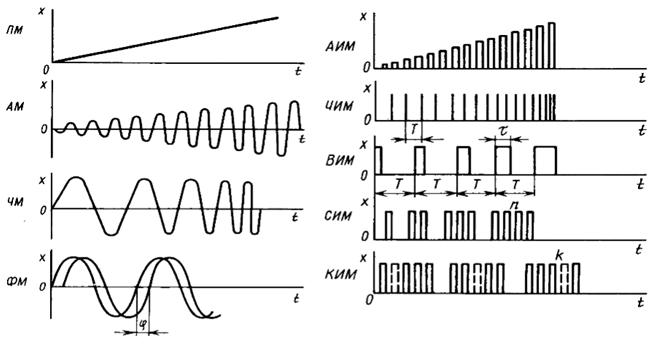
\includegraphics[width=0.7\textwidth]{52.jpg}
\caption{Виды модуляции}
\end{figure}

% Вопрос 53 --------------------------------------------------------
\section{Цифровые частотомеры.}

Цифровые частотомеры являются многофункциональными приборами, в зависимости от режима их работы можно проводить измерение не только частоты, но и интервалов времени (периода следования периодических сигналов). Принцип измерения частоты гармонического сигнала цифровым методом поясняет структурная схема цифрового частотомера в режиме измерения частоты и временные диаграммы к его работе.
\begin{figure}[H]
\centering
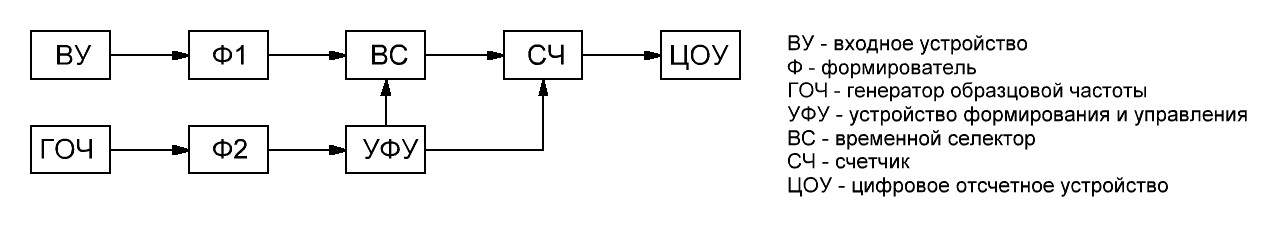
\includegraphics[width=0.9\textwidth]{53.jpg}
\caption{Структурная схема цифрового частотомера}
\end{figure}

Исследуемый гармонический сигнал, имеющий частоту $f_x$ , подается на входное устройство (ВУ), усиливающее или ослабляющее его до значения, требуемого для работы последующего устройства частотомера. Формирователь Ф1 состоит из усилителя-ограничителя и компаратора (триггера Шмитта).

Счетные импульсы поступают на один из входов временного селектора (ВС), на второй вход которого от устройства формирования и управления (УФУ) подаётся строб-импульс прямоугольной формы и калиброванной длительности. Временной селектор открывается строб-импульсом  и в течение его длительности пропускает группу (пакет) импульсов на вход счетчика (СЧ). В результате на счетчик поступает пакет из $N_X$ импульсов.

Для формирования строб-импульса на устройство УФУ поступают короткие импульсы с периодом $T_0$ от схемы, включающей генератор образцовой частоты (ГОЧ) и второй формирователь импульсов (Ф2), аналогичный формирователю Ф1. В составе ГОЧ имеется кварцевый генератор образцовой частоты и декадный делитель частоты. Период импульсов на выходе формирователя Ф2 и длительность строб-импульсов равны периоду сигнала на выходе делителя частоты.

Счетчик подсчитывает $N_X$ импульсов и выдает соответствующий (двоичный) код в цифровое отсчетное устройство (ЦОУ). Циклический режим работы частотомера задаётся УФУ, при этом перед началом каждого измерения УФУ сбрасывает показания счетчика в ноль. Максимальная ошибка - 1 интервал тактового сигнала, то есть определяющим звеном частотомера является опорный генератор.

Для измерения ВЧ сигналов возможен режим работы, при котором заполнение интервала происходит импульсами самого входного сигнала, а ГОЧ формирует точный интервал.

% Вопрос 54 --------------------------------------------------------
\section{Цифровые фазометры.}

Цифровые фазометры предназначены для измерений углов поворота, снятия фазочастотных характеристик различных звеньев. Цифровые фазометры можно разделить на две группы: для измерения мгновенного значения сдвига фаз и для измерения среднего значения сдвига фаз. Сдвиг по фазе $\varphi$ между двумя напряжениями $u_1 (t)$ и $u_2 (t)$ легко преобразуется во временной интервал $\tau$.
Поэтому схема цифрового фазометра отличается от схемы ЦИП для измерения временных интервалов двумя формирователями Ф1 и Ф2, формирующими старт- и стоп-импульсы в момент перехода кривых напряжений $u_1 (t)$ и $u_2 (t)$ через нуль, и блоком выделения временного интервала БВВИ (см. рис.).

\begin{figure}[H]
\centering
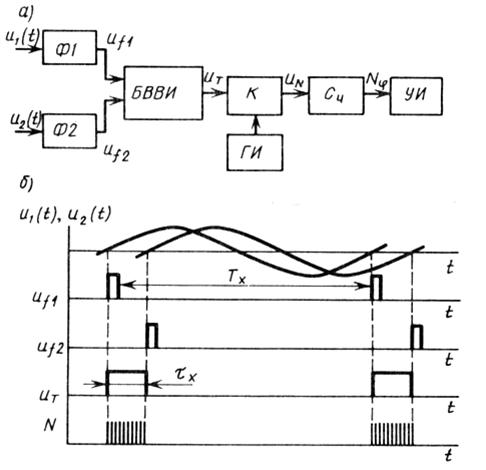
\includegraphics[width=0.65\textwidth]{54.jpg}
\caption{Цифровой фазометр: а - структурная схема; б - временная диаграмма; (БВВИ - блок выделения временных интервалов; Ф - формирователь; К - ключ; ГИ - генератор импульсов; Сч - счетчик; УИ - устройство индикации)}
\end{figure}

В соответствии со структурной схемой, количество импульсов сигнала $U_N (t)$ образцовой частоты $f_0$ с ГИ, поступившее за время $\tau_x$ в счетчик Сч, будет равно $N_X = \tau_x f_0$. Отсюда получаем:
\begin{displaymath}
\varphi_x = \frac{2\pi \tau_x N_X}{f_0}
\end{displaymath}

При измерении фазового сдвига необходимо либо обеспечить постоянство частот измеряемых сигналов $f_1$ и $f_2$, либо обеспечить постоянство отношения $f_x/f_0$.

\section{Цифровые вольтметры временного преобразования.}
\section{Микропроцессорные цифровые измерительные преобразователи.}
\section{Резистивные датчики (реостатные, пьезорезистивные).}
\section{Электромагнитные датчики (индуктивные, трансформаторные, магнитоупругие).}
\section{Пьезоэлектрические датчики.}
\section{Тепловые датчики (термопары, термометры сопротивления).}
\section{Организация и этапы разработки конструкторских документов.}
\section{Виды КД.}
\section{Стандартизация и БНК.}
\section{Виды и типы схем, обозначения по ЕСКД.}
\section{Методы компоновки конструкции ЭВС.}
\section{Климатические зоны и категории исполнения.}
\section{Способы защиты ЭВС от влаги.}
\section{Защита ЭВС от механических воздействий.}
\section{Способы обеспечения теплового режима ЭВС.}
\section{Электромагнитные воздействия. Виды экранов.}
\section{Виды линий связи.}
\section{Особенности конструирования бортовых ЭВС.}
\section{Особенности конструкций персональных ЭВМ.}
\section{Унификация. Разновидности стандартизации.}
\section{Требования к трассировке ПП и электрическим соединениям.}
\section{Электромонтажные провода. Припои и флюсы.}
\section{Волоконно-оптические линии связи (ВОЛС). Примеры использования.}
\section{Эргономические требования к пультам, органам управления и сигнализации.}
\section{Эргономика конструирования лицевой панели прибора.}
\section{Защита ЭС от воздействий радиации.}
\section{Производственный и технологический процесс и их составляющие.}
\section{Исходные данные для разработки технологических процессов. Основные этапы разработки единичного технологического процесса.}
\section{Требования к оформлению технологической документации. Примеры записи технологических операций.}
\section{Основные методы изготовления печатных плат и их особенности.}
\section{Конструктивно-технологические разновидности радиоэлектронных узлов и их сопоставительный анализ.}
\section{Основные технологические операции при изготовлении радиоэлектронных узлов с монтажом на поверхность.}
\section{Нанесение паяльной пасты и клея и используемое при этом оборудование.}
\section{Принципы организации работы сборочных автоматов.}
\section{Особенности выполнения пайки при изготовлении электронных модулей (пайка оплавлением, волной припоя, селективная пайка).}
\section{Особенности выполнения ремонтных работ: демонтаж и монтаж компонентов.}
\section{Материалы, используемые в технологии монтажа на поверхность.}
\section{Виды соединительных операций при сборке.}
\section{Соединение сваркой: разновидности, области применения.}
\section{Соединение пайкой: разновидности, области применения, примеряя выполнения паяных соединений.}
\section{Разработка схемы сборки изделий.}
\section{Нормирование затрат времени при проектировании технологических процессов (штучное и подготовительно-заключительное время, определение такта и ритма выпуска изделий).}
\section{Изготовление деталей ЭС методом литья.}

\section{Разделительные и формообразующие операции холодной штамповки.}

\section{Общая характеристика методов формообразования материалов и деталей при производстве ЭС.}

% Вопрос 100 ---------------------------------------------------------------------------------------------------------------
\section{Изготовление электронных модулей по технологии внутреннего монтажа.}

% Вопрос 101 ---------------------------------------------------------------------------------------------------------------
\section{Приведите структуру контроллера (микроЭВМ) с раздельными шинами адрес/данные и следующим составом: ХХ кб, ПЗУ – ХХ кб, индикация – 1, порты ввода/вывода – Х клавиатура – 1. Распределите адресное пространство для контроллера. Приведите таблицу распределения адресов.}

\begin{figure}[H]
\centering
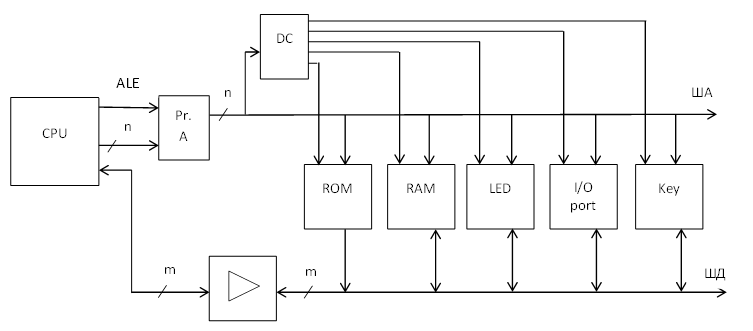
\includegraphics[width=0.8\textwidth]{101_struct.png}
\end{figure}

Допустим шина адреса процессора включает 16 бит, а шина данных – 8 бит, тогда максимальный объем адресуемой памяти составит 64 Кбайт. Предположим что для ОЗУ необходимо выделить 32 Кбайта, ПЗУ – 8 Кбайт, индикация – 256 байт, порт ввода/вывода – 256 байт, клавиатура – 256 байт. При делении адресного пространства между блоками необходимо соблюдать, чтобы начальный адрес каждого блока начинался с нулей, а старший заканчивался на “F”.

\begin{center}
\begin{tabular}{|c|c|c|}
\hline 4000h - AFFFh & ОЗУ                 &  32 Кбайт  \\
\hline 3200h - 32FFh & порт ввода/вывода   &  256 байт  \\
\hline 3100h - 31FFh & клавиатура          & 256 байт   \\
\hline 3000h - 30FFh & индикация           & 256 байт   \\
\hline 1000h - 2FFFh & ПЗУ                 &  8 Кбайт   \\
\hline 0000h - 0FFFh & регистры процессора & 4 Кбайт    \\
\hline
\end{tabular}
\end{center} 

% Вопрос 102 ---------------------------------------------------------------------------------------------------------------
\section{Укажите место на структурной схеме ЭВМ различных интерфейсов. Как объединять ЭВМ в  систему? Какие условия следует выполнить при  передаче данных? Обоснуйте.}

\begin{figure}[H]
\centering
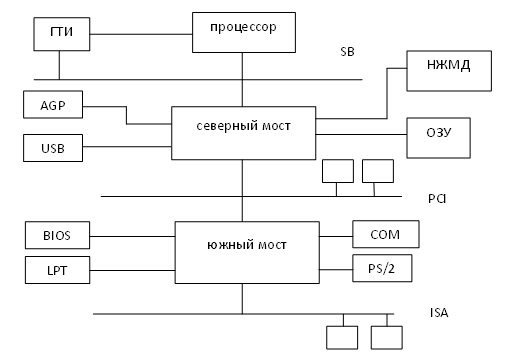
\includegraphics[width=0.8\textwidth]{./images/102_interface.png}
\end{figure}

В структуре ЭВМ в зависимости от назначения используются следующие интерфейсы:
\begin{enumerate}
\item Межпроцессорные интерфейсы – для объединения нескольких процессоров: шинный интерфейс с адресным арбитражем(по командам).
\item Межсистемный интерфейс – для объединения нескольких вычислительных блоков в одну систему. Задача возникает в кластерах. Необходим быстрый \item коммутатор и сеть типа 1 Гбит.
\item Системные интерфейсы – набор шин с правилами обмена между основными блоками ЭВМ.
\item Интерфейсы ВУ (периферийные) – обмен информации между системным блоком и ВУ.
\item Территориальные – связь с ВУ за корпусом ЭВМ, либо с внешними устройствами встроенными в корпус.(COM, USB, LPT, PS/2).
\end{enumerate}

При проектировании и реализации схемы интерфейса необходимо выполнить три условия согласования для передачи от устройства к приемнику:
\begin{enumerate}
\item Механические
\item Логические
\item Электрические
\end{enumerate}

Механические --- тип разъема, число контактов, расстояние между ними.

Логические --- последовательность передачи сигналов и наличие сигналов синхронизации определяется протоколом интерфейса, форматом передаваемого кадра и в конечном счете программным управлением. Уровни <<1>> и <<0>> так же определяются логическими условиями.

Электрические --- временные положения импульсов, величина фронтов, длительность сигналов синхронизации, фазовые сдвиги.

Помимо условий согласования необходимо выполнить интерфейсные функции: на время в буфере сохранить сигнал, проанализировать ответный сигнал, сформировать сигнал сопровождения и т.д.

% Вопрос 103 ---------------------------------------------------------------------------------------------------------------
\section{Расставьте по убыванию значимости параметры ЭВМ по критерию производительности. Охарактеризуйте эти параметры.}

Производительность – число операций выполняемых в единицу времени. Если данные представлены в целом коде – единица измерения MIPS (миллион инструкций в секунду). Если данные представлены в  формате ПЗ – единица измерения FLOP (операций в секунду). Производительность комьютера не вычислияется, а определяется в процессе тестирования по скорости выполения определенных операций в программной среде.
Параметры влияющие на производительность ЭВМ:
\begin{enumerate}
\item Операционные ресурсы
\item Емкость памяти ресурсы
\item Разрядность шины адреса и данных
\item Быстродействие
\item Память
\end{enumerate}

Операционные ресурсы – это перечень действий, которые может делать (выполнять) аппаратура ВС в плане обработки информации (исходных данных). В этот перечень прежде всего включается система машинных операций – список F=\{+,-,*,/,…\}. Кроме того, это порождающая ее (систему операций) система машинных команд К=\{К1, …, КN\}. В понятие операционные ресурсы включаются также способы представления информации в ЭВМ, способы представления чисел, текстов, логических значений. Чем шире перечень действий, чем шире многообразие способов представления данных – тем шире операционные ресурсы ЭВМ и, следовательно, возможности ВС в плане обработки информации.

Емкость памяти – очевидная техническая характеристика, которая характеризует вместимость хранилища программ и данных ВС. Единицы измерения – бит,  байт,  килобайт , мегабайт,  гигабайт, терабайт.  Емкость  памяти $ E $ обычно  кратна степени 2: $ E = 2^{m}$, $ m $ – длина (разрядность) адреса.

Разрядность шины адреса и данных – определяет количество бит передаваемых шиной. Чем больше разрядность, тем большее количество информации можно передать за один такт.

Быстродействие – это характеристика, которая отвечает на вопрос, как быстро действует (работает) аппаратура ЭВМ. Эта характеристика определяет потенциальные возможности устройств, указывает на верхнюю границу. Относится к отдельным устройствам, а не ВС в целом. Так, быстродействие процессора характеризует скорость, с которой это устройство может выполнять операции: Быстродействие определяется количеством операций в единицу времени и зависит от времени выполнения операции: $ V=1/t $ – чем меньше время выполнения операции t, тем выше быстродействие. Быстродействие процессора определяется временем выполнения команд. Память ЭВМ предназначена для хранения, записи и чтения информации. Быстродействие памяти принято характеризовать количеством операций чтения/записи в единицу времени. Память ЭВМ строится на базе ЗУ (БИС ОЗУ, ППЗУ). Быстродействие памяти зависит от быстродействия ЗУ и ее внутренней организации. 

% Вопрос 104 ---------------------------------------------------------------------------------------------------------------
\section{Преобразуйте десятичное число в различные форматы хранения. В какой форме хранятся в памяти ЭВМ символы. Приведите два примера.}

Методика преобразования целых десятичных чисел в двоичные коды различна в зависимости от знака числа.

Положительные числа имеют одинаковое представление в обратном, прямом и дополнительном кодах, и имеют цифру $ 0 $ в знаковом разряде: $ 127_{10}=01111111_{2} $.

Отрицательные числа представляются в виде дополнительного кода. Преобразование из прямого кода в дополнительный сводится к следующим действиям:
\begin{enumerate}
\item Прямой код

В знаковый разряд помещается цифра $ 1 $, а в разряды цифровой части числа – двоичный код абсолютной величины: $ -127_{10}=11111111_{2} $
\item Обратный код

Получается инвертированием всех цифр двоичного кода без учета знакового разряда: нули заменяются единицами и наоборот: $ -127_{10}=10000000_{2} $
\item Дополнительный код

К обратному коду добавляется единица к младшему разряду: $ -127_{10}=10000001_{2} $.
Дополнительный код и есть представление отрицательного числа $ -127 $.
\end{enumerate}  

Преобразование вещественных чисел со знаком:

Вещественное число $ X $ можно представить в виде произведения мантиссы $ m $ и основания системы счисления $ q $ в некоторой степени $ n $ : $ X=m \ast q^{n} $. 
Например: $ 25.324 = 0.25324\ast 10^{2} $. Здесь $ 0.25324 $ – нормализовання мантисса, $ 2 $ – порядок(степень). Порядок указывает, на какое количество позиций должна сместиться запятая в мантиссе. Необходимо, чтобы значение мантиссы было нормализованно и удовлетворяло условию: $ 0.5 \leq m < 1 $. Другими словами нормализованная мантисса меньше $ 1 $ и первая значащая цифра после запятой не меньше $ 5 $. 
Двоичный код вещественного числа должен быть следующего формата:

\begin{center}
\begin{tabular}{|c|c|c|}
\hline 8 бит   & 1 бит & 23 бит   \\ 
\hline порядок & знак  & мантисса \\ 
\hline 
\end{tabular}
\end{center}
 
Допустим имеем число $278.15$, переведем его в двоичный код в формате п.з.. Подставим это число в формулу $ X=m\ast q^{n} $. Получим уравнение:$278.15= m\ast q^{n}$. Для нахождения мантиссы $m$ неизвестен порядок $n $, найдем его: $2^{8}=256$, что меньше $278.15$, возьмем следующую степень по порядку $-2^{9}=512$. В данном случае $512>278.15$, по этому выберем $q^{n}=2^{9}$. Тогда мантисса $m=X/q^{n} =278.15/512=0.543$. Прямой код мантиссы $m=0.543=10001_{2}$. Прямой код порядка $n=9=1001_{2}$. Теперь можно записать число в формате с плавающей запятой:

\begin{center}
\begin{tabular}{|c|c|c|}
\hline порядок  & знак & мантисса                \\ 
\hline 00001001 & 0    & 10001000000000000000000 \\ 
\hline 
\end{tabular}
\end{center}

Преобразование в шестнадцатеричные коды:

Преобразование из двоичного кода в шестнадцатеричный производят в два этапа: перевод в двоичный код, а затем уже в шестнадцатеричный.

Для преобразования из двоичного кода в шестнадцатеричный нужно условно разбить код на тетрады. Например, необходимо преобразовать код: $ 110100011,1111_{2} $. Разбиваем его на тетрады: $ 1 \mid 1010 \mid 0011 \mid 1111 $. И каждую тетраду заменяем на соответствующее шестнадцатеричное число. $ 1_{2} = 1_{16} $, $ 1010_{2} = A_{16} $, $ 0011_{2} = 3_{16} $, $ 1111_{2} = F_{16} $. В итоге получим число $ 1A3,F $. В таблице указано соответствие двоичных чисел шестнадцатеричным:

\begin{center}
\small
\begin{tabular}{|c|c|c|c|c|c|c|c|c|c|c|c|c|c|c|c|}
\hline 0000 & 0001 & 0010 & 0011 & 0100 & 0101 & 0110 & 0111 & 1000 & 1001 & 1010 & 1011 & 1100 & 1101 & 1110 & 1111 \\ 
\hline 0 & 1 & 2 & 3 & 4 & 5 & 6 & 7 & 8 & 9 & A & B & C & D & E & F \\ 
\hline 
\end{tabular}
\end{center}

Преобразование в двоично-десятичный код:

Преобразование десятичного числа в двоично-десятичный код осуществляется переводом каждого разряда десятичного числа в соответствующий четырехбитовый эквивалент. Например, число $ 311_{10} = 011100010001_{BCD} $. Здесь  $3_{10} = 0111_{2}$, $1_{10} = 0001_{2}$.

Хранение символов в ЭВМ:

Каждая буква принадлежит определенному алфавиту, в котором символы следуют друг за другом и, следовательно, могут быть пронумерованы последовательными целыми числами. Каждой букве можно сопоставить целое положительное число и назвать его кодом символа. Именно этот код будет храниться в памяти компьютера, а при выводе на экран или бумагу «преобразовываться» в соответствующий ему символ. Чтобы отличить представление чисел от представления символов в памяти компьютера, приходится также хранить информацию о том, какие именно данные закодированы в конкретной области памяти.

Соответствие букв определенного алфавита с числами-кодами формирует так называемую таблицу кодирования. Другими словами, каждый символ конкретного алфавита имеет свой числовой код в соответствии с определенной таблицей кодирования. Американским национальным институтом стандартизации (ANSI) была разработана таблица кодирования символов, которая впоследствии была использована во всех операционных системах. Эта таблица называется ASCII.

Например, символу $A$ соответсвует код 41h, а символу $+$ код 2Bh. 

% Вопрос 105 ---------------------------------------------------------------------------------------------------------------
\section{Сопоставьте принципы печати лазерного и струйного принтеров, опишите и сравните их.}

{\bf Лазерный принтер:}

В основе печати лазерным способом лежит принцип переноса изображения из кодов на образующую фотобарабана лазерным лучом. Луч двигается слева направо(принцип монитора) при этом модулируется так же знакогенераторм или графическим процессором, барабан перемещается всякий раз на одну линию и далее уже красящее вещество с барабана механически переносится на бумагу. Печатающий узел называется катридж. Основа в катридже - кожух с продольным отверстием, которое закрывается шторкой. При сдвиге шторки через отверстие виден барабан светлого света, покрытый селеном потому, что он под воздействием света проявляет внешний фотоэлектрический эффект. Помимо барабана в кожухе размещается красящий порошок - тонер - мелкодисперсный синтетический состав, плавящийся при нагревании. С торцов катриджа система шестерен для управления вращением барабана. Так же в катридже расположен электрод, на который подается высокое отрицательное напряжение. Коды символов, поступая в процессор принтера преобразовываются в управляющую последовательность кодов. Эта последовательность единиц и нулей посылается на лазер - источник света с тонким лучом. Луч направлен на зеркало, которое перемещает его строго по образующей барабана с одного конца на другой. Подавая 1 и 0 на лазер, формируются светлые и темные точки на образующей цилиндра.
\begin{figure}[H]
\centering
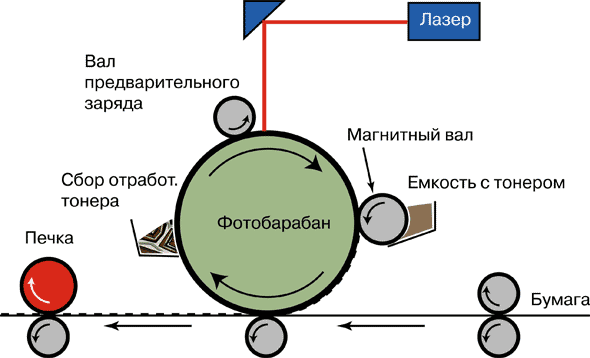
\includegraphics[width=0.6\textwidth]{105_Laser.png}
\caption{Лазерный принтер}
\end{figure}
В начальном состоянии барабан не заряжен, тонера на нем нет. Но рядом с барабаном имеется электрод, заряжающий барабан отрицательно. При вращении барабана его поверхность заряжается равномерно. При печати луч лазера попадает через зеркало на образующую барабана и выбивает электроны в том месте куда он попал. После того как пройдет развертка, формируются заряженные и незаряженные точечки. При дальнейшем движении сверху сыплется порошок, имеющий отрицательный заряд. При соприкосновении с поверхностью цилиндра порошок прилипает к его незаряженным частям. Барабан вращается дальше, и в нижней точке соприкасается с листом бумаги, образуя оттиск на бумаге - барабан вдавливается в бумагу. Бумага двигается далее по роликам нагревается, и, порошок расплавляясь, въедается в бумагу. Поскольку развертка движется периодически, на поверхности барабана получаем рисунок, символы в котором непрерывным путем переносятся на бумагу.

Преимущество: скорость печатания лазерных принтеров велика - до нескольких десятков страниц в минуту. Разрешающая способность 300-1200 dpi. Являются экономичными.

Недостаток: один тонер. Поэтому для цветной печати выполняют три пишущих узла, с разными тонерами (RGB). Цвета наносятся друг за другом  и затем сплавляются. 

{\bf Струйный принтер:}

Развитием в сторону бесконтактного способа матричной печати (иголок), является печать капельками жидкости - струйные принтеры. У таких принтеров капельки красящего вещества выстреливают из сопла головки, пролетают небольшое расстояние и попадают на бумагу. Основная проблема в таких устройствах печати - это то, как "прилепить" каплю жидкости к бумаге. В струйных принтерах бумага должна быть не очень плотной, и в то же время иметь плотность не хуже некоторого значения, по скольку жидкость распространяется во все стороны. Задача решается совместно: определенное качество бумаги и текучести чернил. По скольку капелька вытекает из сопла, то можно размещая по три сопла рядом печатать цветом. На практике существуют два способа струйной печати: {\sl Непрерывная и импульсная струйная печать.}

{\sl Непрерывная струйная  печать:}

Чернила подаются в печатающую головку с помощью насоса. Возникающая под создаваемым им давлением струя разбивается на капельки за счет вибрации, вызываемой, например, пьезоэлектрическим элементом. Разумеется, до бумаги должны долететь не все, а только часть капелек, иначе никакого изображения не получится - бумага просто будет равномерно залита чернилами.
Вылетая из сопла, капельки проскакивают через заряжающий электрод. Получив электрический заряд, они попадают в поле отклоняющего электрода, на который подается высокое напряжение. Изменяя напряжение на отклоняющем электроде, можно заставить капельки поменять траекторию полета. Если состоящая из заряженных капелек струя не отклоняется в сторону, она попадает в уловитель, из которого неиспользованные чернила стекают в накопитель, проходят стадию удаления воздушных пузырьков (дегазации) и снова сливаются в основной резервуар с краской.
Сменившие направление полета под действием электрического поля отклоняющего электрода капельки попадают на бумагу, формируя на ней изображение. Угол отклонения траектории зависит от того, насколько сильно изменяется напряжение.
Системы непрерывной струйной печати отличаются тем, что в них применяется дорогая электропроводная краска, способная получить заряд. Так как между соплом и бумагой необходимо разместить два электрода, увеличивается дальность полета капелек и, следовательно, им необходимо придать большую начальную скорость. Очень высока и производительность сопел печатающей головки - из них в секунду вылетает от 50 до 150 тысяч капелек. Однако сам процесс печати не назовешь очень быстрым.

Недостаток: медленная печать, серьезные эксплуатационные расходы, обусловленные дороговизной чернил и сложностью обслуживания таких принтеров, и, конечно, немалая цена самого оборудования.

Преимущество: высокое качество получаемых с ее помощью цветных изображений.

{\sl Импульсная струйная печать:}

Капельки из сопел пьезоэлектрической головки вылетают под воздействием создаваемого на очень короткое время избыточного давления в камере с чернилами. Для образования в камере избыточного давления применяется диск из пьезоэлектрика. Когда к нему подводится напряжение, он деформируется (изгибается). Выгнувшись, диск, который служит одной из стенок камеры с чернилами, резко уменьшает ее объем, оказавшиеся лишними чернила вылетают при этом из сопла в виде капельки. Для заполнения камеры, когда напряжение снято и пьезоэлектрический диск возвращается к исходной форме, применяется капиллярный способ подачи чернил из резервуара. 

\begin{figure}[H]
\centering
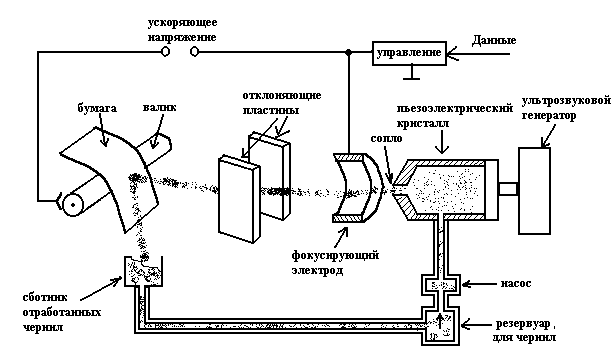
\includegraphics[width=0.6\textwidth]{105_Strui.png}
\caption{Струйный принтер на основе пьезоэлектрика }
\end{figure}

Конструкция современных пузырьковых головок допускает использование быстро сохнущих чернил, благодаря чему капельки не успевают впитаться в бумагу или растечься - они просто моментально высыхают. Благодаря увеличению скорости, с которой из сопел выстреливаются капельки, можно увеличить зазор между головкой и бумагой. Больший зазор позволяет применять бумагу худшего качества, неровную или более плотную.Такая технология привела к упрощению конструкции, удешевлению самих принтеров, так и к снижению эксплуатационных затрат.

\section{Приведите две схемы подключения клавиатуры к портам ввода-вывода. Приведите алгоритм опроса пассивной матричной клавиатуры.}

% Вопрос 106 ---------------------------------------------------------------------------------------------------------------
Схема подключения клавиатуры через регистр с прерыванием:

Тактовый сигнал непрерывно пишет в регистр состояние кнопок, в то время как $cs$ пока не открывает выход. По нажатию кнопки, сигнал прерывания поступает в процессор, который запускает подпрограмму обработки клавиатуры. Процессор выставляет адрес закрепленный за клавиатурой, адресный дешифратор формирует $cs$, и на выходе регистра появляется состояние кнопок. Сигналы с выхода регистра поступают в какой либо внутренний регистр процессора, определяется один или несколько активных разрядов и соответствующая кнопка. 

\begin{figure}[H]
\centering
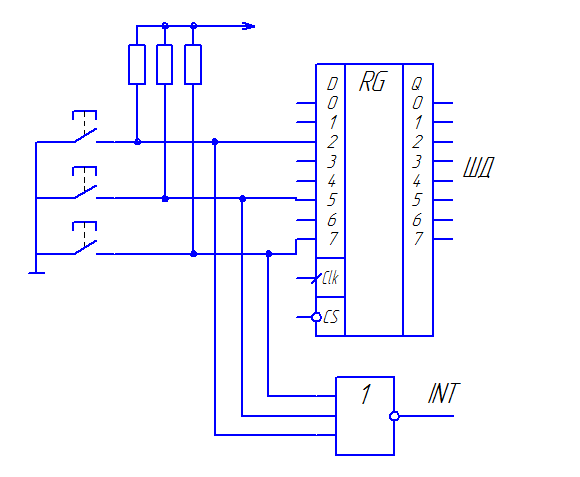
\includegraphics[width=0.4\textwidth]{106_Button.png}
\caption{Подключение кнопок через регистр с прерыванием}
\end{figure}

Схема подключения матричной клавиатуры

Пассивная матрица $4\times 3$ имеет 4 строки и 3 столбца. На пересечении столбец/строка стоит кнопка, не обязательно гальванический контакт, возможен емкостный.

По каналу А в порт отправляем из процессора сканирующий код следующей структуры: $1110,{} 1101,{} 1011,{} 0111$. Выставив первый код, мы читаем по каналу В состояние разрядов. При появлении 0 на $A0$ и замыкании верхнего ключа, разряд $B0$ становится низким по скольку ток с контакта $+5B$ течет через резистор и диод на $A0$. Читая код по $B$ определяем есть ли в нем 0 и в каком разряде. Если в возбужденной строке появился 0 значит одна из трех кнопок в возбужденной строке замкнута, осталось определить которая. Чтобы определить которая кнопка замкнута необходимо последовательно маскировать каждый из разрядов порта $B$. Конкретный разряд умножаем на 1 а другие на 0 и смотрим 1 или 0 в данном разряде. Если 0 то через таблицу присвоения символа определяем какая нажата, выполняя подпрограмму. Сочетание активной строки и 0 в принятом столбце дает указанную кнопку.

\begin{figure}[H]
\centering
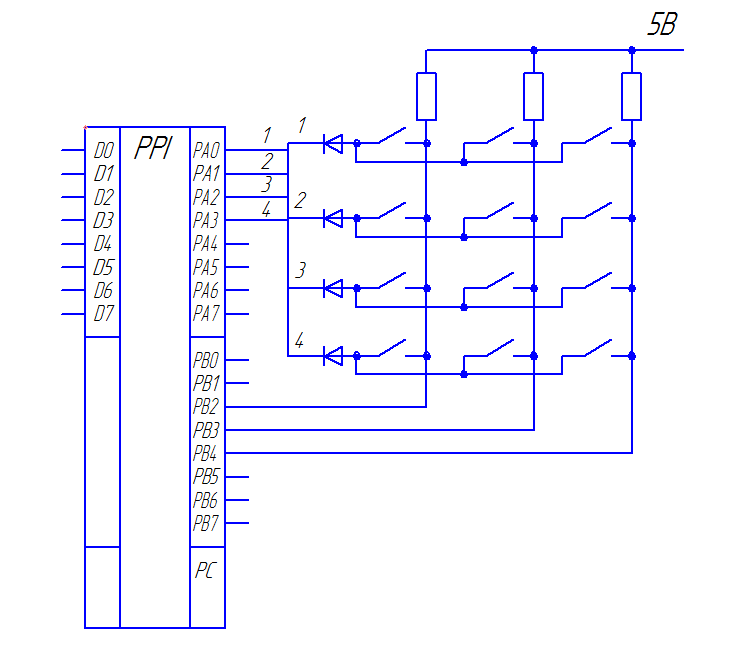
\includegraphics[width=0.4\textwidth]{106_Keyboard.png}
\caption{Матричная клавиатура}
\end{figure}

% Вопрос 107 ---------------------------------------------------------------------------------------------------------------
\section{Выберите способ обмена данными между процессором и внешним устройством. Обоснуйте выбор. Напишите процедуру ввода или вывода данных в память ЭВМ в мнемонике команд (уровень ассемблера).}

Задача обмена данными между внешним устройством и процессором сводится к пересылке данных между памятью внешнего устройства(ВУ) и памятью ОЗУ. Существует 3 подхода к обмену информации между процессором и ВУ: программный обмен, ввод/вывод с отображением в память, прямой доступ к памяти (ПДП). Из этих способов предпочтительней является ПДП.

ПДП отличается от предыдущих методов тем, что не задействует процессор при обмене информацией. Функцию процессора на время обмена данными ВУ-ОЗУ выполняет контроллер ПДП. Контроллер представляет собой небольшой автомат, имеющий внутренний счетчик с начальным установом и логику проверки конца счета. 

Последовательность работы заключается в следующем:

Программа формирует сигналы прерывания процессору. Программное прерывание служит сигналом процессору и тот переводит выводы в третье состояние. Если же ввод идет по инициативе внешнего устройства, то ВУ посылает прерывание на процессор. Может быть так что ВУ посылает запрос на контроллер ПДП, который формирует прерывание на процессор. 

Процессор переводит выходные разряды в третье состояние, но перед этим посылает по адресу ПДП по шине данных режим работы и начальный адрес массива памяти, объем, либо конечный адрес. Эти три величины пишутся в контроллере и настраивают его на направление и начальный адрес. После перевода шин в третье состояние, контроллер выставляет начальный адрес на шину адреса, сигнал управления, и выводы внешнего устройства напрямую подключаются к шине данных. Цикл обмена по времени занимает 1 такт работы процессора - скорость обмена максимальная. Обмен производится до тех пор пока не отработает последний адрес. После чего контроллер посылает на процессор сигнал отмены прерывания. Процессор продолжает работу.

\begin{figure}[H]
\centering
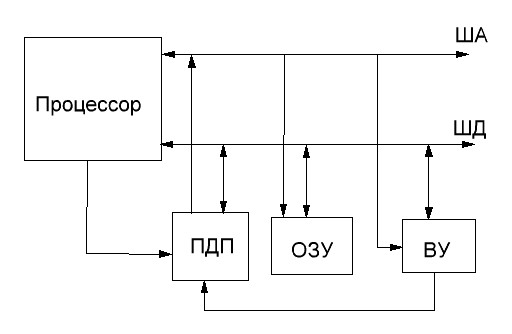
\includegraphics[width=0.4\textwidth]{107_PDP.JPG}
\caption{Ввод/вывод с контроллером ПДП}
\end{figure}  

Процедура ввода данных в память ЭВМ:

\begin{center}
\begin{tabular}{l l}
    & {} M100          \\ 
101 & {} MVI E, 00h    \\ 
102 & {} LXI H, 0020h \\ 
103 & {} MOV M, E      \\ 
104 & {} INR E         \\ 
105 & {} INX H        \\ 
106 & {} MOV A, E      \\ 
107 & {} CPI 80h       \\ 
108 & {} JZ 103        \\  
\end{tabular} 
\end{center}

Процедура последовательно вводит в память начиная с адреса 2000h числа от 00h до 80h. По команде MVI E, в регистр E записывается число 00h. Начальный адрес ячейки памяти 2000h копируется с помощью команды LXI в регистр HL. По скольку первый байт операнда записывается в регистр L, а второй - в регистр H, мы записали этот операнд в виде 0020h. Используя MOV M, копируется число из региcтра E в ячейку памяти, адрес которой содержится в регистре HL. Чтобы записать следующее число в следующую ячейку памяти, производим опреацию инкрементирования. По команде JZ каждый раз происходит переход на операцию ввода данных в ячейку памяти MVI E, но только до тех пор пока не запишется последнее число 80h. Благодаря команде CPI можно проверить конец вводимых в память значений. 

% Вопрос 108 --------------------------------------------------------
\section{Приведите основные архитектурные варианта построения операционных систем. Поясните понятие <<виртуальная машина>>.}
\begin{enumerate}
\item Монолитные системы (монолитное ядро, monolithic kernel) - представляет собой простейшую структуру, когда компоненты операционной системы являются не самостоятельными модулями, а составными частями одной программы. Операционная система написана в виде набора процедур.
\item Многоуровневые системы - является организация операционных систем в виде иерархии уровней.
\item Виртуальные машины.
\item Экзоядро - реализован принцип обеспечения каждого пользователя абсолютной копией реального компьютера, но с подмножеством ресурсов. На нижнем уровне в режиме ядра работает программа – экзоядро (exokernel), в задачу которой входит распределение ресурсов для виртуальных машин и проверка их использования (отслеживание попыток машин использовать чужой ресурс).
\item Ядро в привилегированном режиме - Операционная система должна иметь по отношению к приложениям определенные привилегии, иначе некорректно работающее приложение может вмешаться в работу операционной системы и разрушить часть ее кодов. Аппаратура компьютера должна поддерживать как минимум два режима работы – пользовательский (user mode) и привилегированный (режим ядра, kernel mode или режим супервизора, supervisor mode). Так как ядро выполняет все основные функции операционной системы, то чаще всего именно оно работает в привилегированном режиме.
\item Многослойная структура операционной системы - вычислительная система, работающяя под управлением операционной системы на основе ядра, можно рассматривать как систему, состоящую из трех иерархически расположенных слоев: нижний слой образует аппаратура, промежуточный – ядро, верхний – утилиты, обрабатывающие программы и приложения. При такой организации приложения не могут непосредственно взаимодействовать с аппаратурой, а только через слой ядра.
\item Микроядерная архитектура  -  большинство составляющих операционной системы являются самостоятельными программами Взаимодействие между программами операционной системы обеспечивает специальный модуль ядра – микроядро. Микроядро работает в привилегированном режиме и обеспечивает взаимодействие между программами, планирование использования процессора, первичную обработку прерываний, операции ввода-вывода и базовое управление памятью. Остальные компоненты системы взаимодействуют друг с другом путем передачи сообщений через микроядро.
\item Модель клиент-сервер - операционные системы в кторых происходит перенос большинства задач на операционной системы на средства пользовательских процессов.
\item Смешанные системы - операционные системы использующие различные комбинации перечисленных подходов.


Виртуальные машины.


\end{enumerate} 
% Вопрос 109 --------------------------------------------------------
\section{Спроектировать устройство управления программного типа. Число микрокоманд в цикле – не более 7. Привести примеры циклов: выборка команды, чтение памяти и запись в память. Чем определяется период следования тактового сигнала.}

% Вопрос 110 --------------------------------------------------------
\section{Спроектировать устройство микропрограммного управления автономного типа. Источник управляющих кодов – счетчик микрокоманд, число состояний счетчика – 32. Разрядность регистра микрокоманд – 24.}

%Вопрос №111-------------------------------------------------------------------------------------
\section{Привести примеры процедур с различными способами адресации для пересылки содержимого ячейки памяти команд в ячейку памяти данных в мнемонике команд, адресация в пределах одной страницы (64 кб). Пояснить необходимость модификации адресов для доступа к данным и возможные их способы.}

В памяти команд лежат константы, которые понадобятся в дальнейшем выполнении программы.\\
MVI A,3E\\
STA 12ED\\
В данном примере байт константы (3Е) записывается сначала в аккумулятор процессора, а затем из него в ячейку памяти по адресу 12ED.

Команда MVI A,(d8) -- непосредственная адресация, записывает константу, расположенную в памяти команд  следующей после КОП.
%однострочная аблица с КОП
\begin{center}
\begin{tabular}{|c|c|}
\hline КОП  & data 8 бит \\  
\hline 
\end{tabular}
\end{center}
Команда STA -- \underline{прямая адресация}, записывает значение аккумулятора по адресу указанному в следующих 2 байтах после КОП.
\begin{center}
\begin{tabular}{|c|c|}
\hline КОП & адрес 16 бит \\ 
\hline 
\end{tabular}
\end{center}
MVI A,7C\\ 
STAX B\\
В этом примере байт константы (7С) записывается сначала в аккумулятор процессора, а затем из него в ячейку памяти по адресу расположенному в регистровой паре ВС.

Команда STAX B -- \underline{косвенная адресация}, записывает в ячейку памяти данных значение аккумулятора, по адресу, расположенному в регистрах ВС.
\begin{center}
\begin{tabular}{|c|}
\hline КОП \\ 
\hline 
\end{tabular}
\end{center}
MVI M,43\\
MVI M -- команда \underline{непосредственно-косвенной адресации}, когда константа , лежащая в памяти команд записывается в ячейку памяти данных.
\begin{center}
\begin{tabular}{|c|c|}
\hline КОП & data 8 бит \\ 
\hline 
\end{tabular}
\end{center}

Модификации адресов произошла в следствии увеличения объема адресуемой памяти. Всю память поделили на страницы фиксированной длинны и для её адресации используются новые методы.

\underline{Страничная адресация} -- адрес получается путем присоединения значения ячейки в странице к номеру страницы. adr = l.m\\
\begin{figure}[H]
\centering
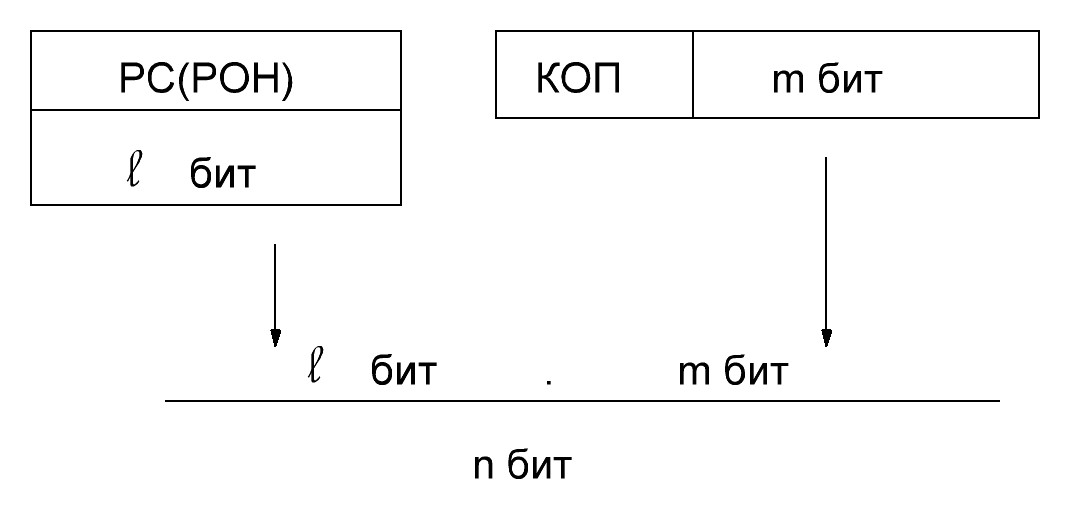
\includegraphics[width=0.6\textwidth]{111_Stranichna.JPG}
\caption{Получение физического адреса}
\end{figure}
При ША равной n бит , n= l + m , где l бит-номер страницы, а m бит-ячейка в странице.

Номер страницы хранится в специальном регистре, так же он может быть и в РОН, а номер ячейки указывается в адресном поле команды.
Страничная адресация имеет следующие достоинства:
\begin{enumerate}
\item Перемещаемость программ и данных обеспечивается путем занесения номера текущей страницы в регистр номера страницы.
\item Длина поля ячейки страницы небольшая и постоянная m < n.
\item Расширение адресного пространства при небольшом адресном поле в команде.
\end{enumerate}
Недостатки страничной адресации:
\begin{enumerate}
\item Сложности с организацией переходов в программе за пределы страницы, нужно изменять содержимое регистра номера страницы, что приводит к снижению быстродействия.
\item не эффективное использование памяти , т.к. распределение между задачами происходит постранично, поэтому часть последней страницы может пустовать. 
\end{enumerate}

\underline{Относительная адресация} -- образует адрес путем смещения относительно начала страницы. Физический адрес получается при сложении значения  смещения, находящегося в поле адреса команды, и значения базового  адреса, находящегося в базовом регистре процессора.\\
adr(n бит) = B(n бит) + D(n бит), где В - значение базового адреса(начало страницы), D - значение смещения.

Страничная адресация является частным случаем относительной. 
\begin{figure}[H]
\centering
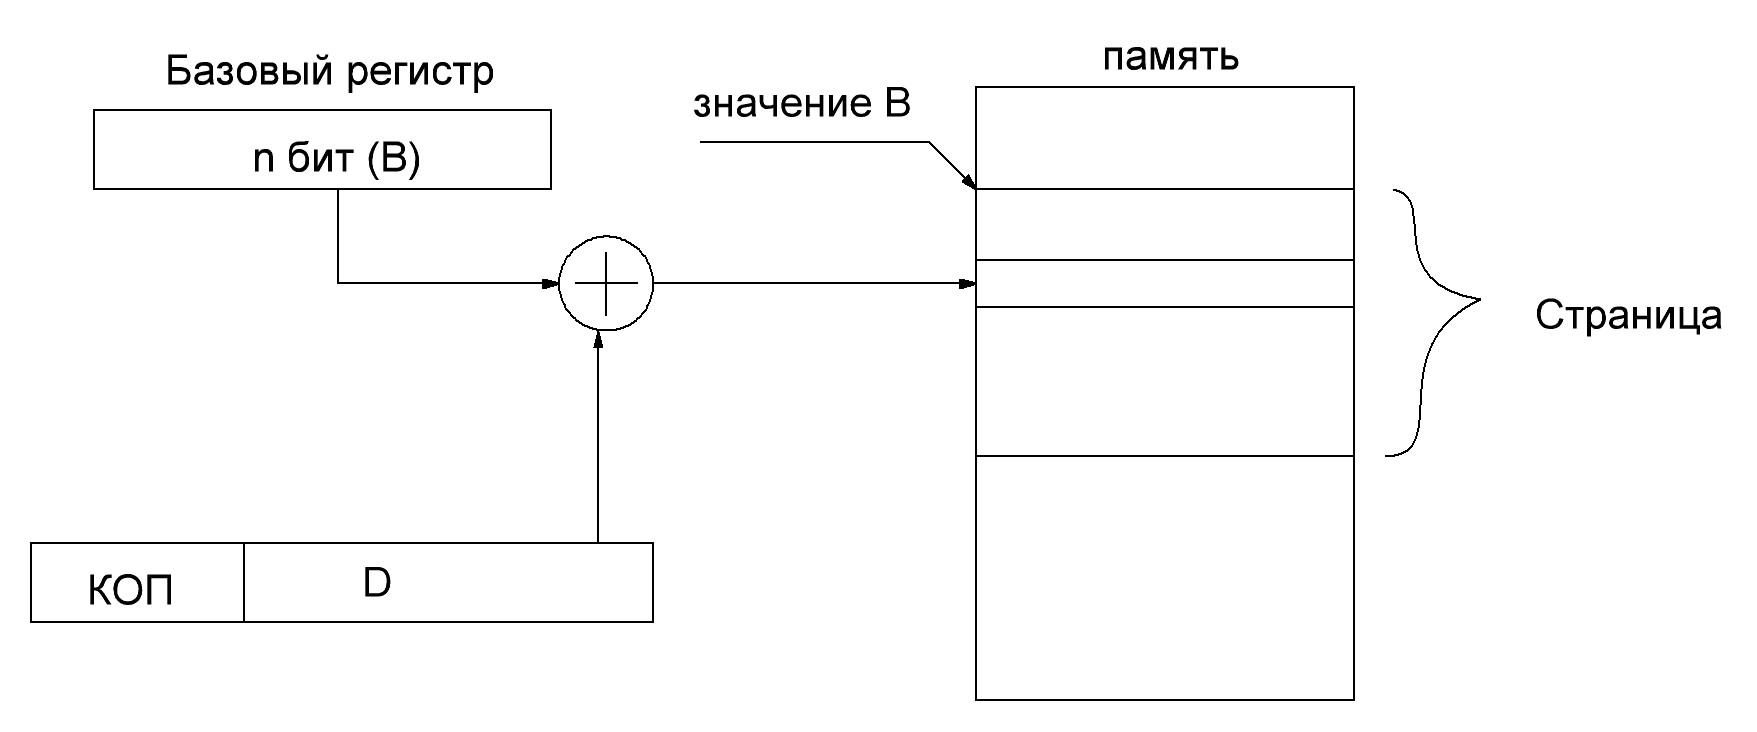
\includegraphics[width=0.6\textwidth]{111_Otnositelna.JPG}
\caption{Получение физического адреса}
\end{figure}


\underline{Индексная адресация} -- используется для адресации элементов массивов. Физический адрес получают путем сложения значения базового адреса, находящегося в поле адреса команды, и значения индексного регистра.\\
\begin{figure}[H]
\centering
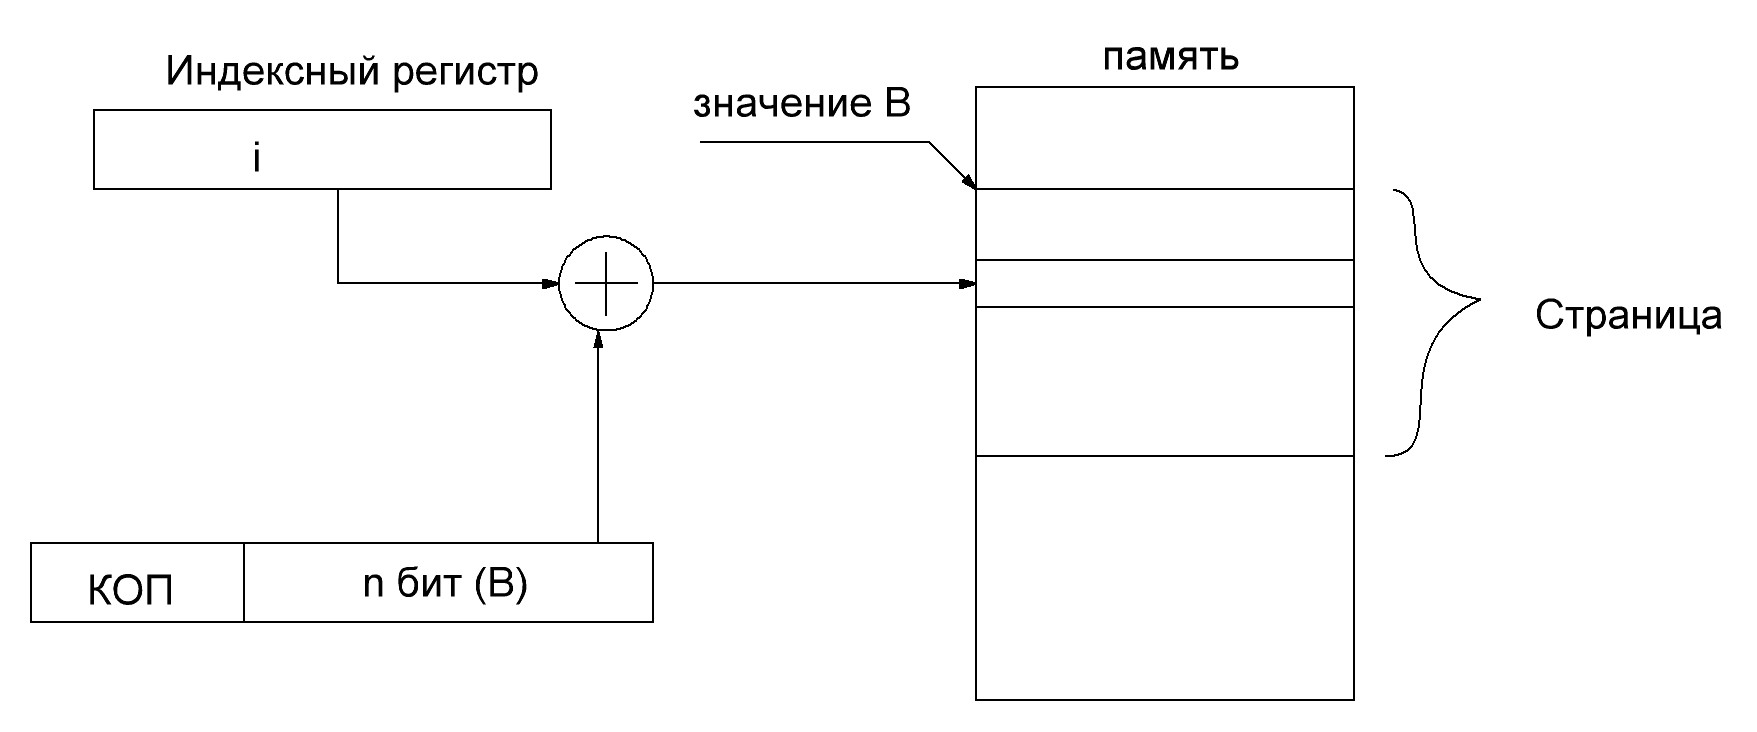
\includegraphics[width=0.6\textwidth]{111_Indexna.JPG}
\caption{Получение физического адреса}
\end{figure} 
\underline{Индексно-относительная адресация} -- совместное использование индексной и относительной адресации. 
adr = i + B + D, где i-индекс, В-базовый адрес, D-смещение.

Все модифицированные способы адресации направлены на формирование адреса за минимальное время при максимальном адресном пространстве. В системе DEC присутствует два дополнительных способа адресации : автоинкрементный и автодекрементный. При косвенной адресации происходит увеличение или уменьшение значения адресного регистра после каждого обращения в память.

% Вопрос 112 --------------------------------------------------------
\section{Прерывания как способ изменения адреса в управляющей команде. Привести пример системы прерывания. Описать процедуру опознавания запроса на прерывание с маскированием.}

% Вопрос 113 --------------------------------------------------------
\section{Системы памяти ЭВМ. Назначение каждого типа элементов памяти и место его в иерархии. Что дает для характеристик ЭВМ каждый тип элементов памяти.}

% Вопрос 114 --------------------------------------------------------
\section{Память программ. Виды носителей. Жесткие диски и их твердотельные аналоги.}

% Вопрос 115 --------------------------------------------------------
\section{Компиляторы. Назначение компиляторов, их виды. Последовательность процедуры компиляции.}

% Вопрос 116 --------------------------------------------------------
\section{Контроль информации при последовательной передаче двоичного кода. Методы контроля. Контроль передачи информации при обмене словами (байтами). Методы.}

Считается, что цифровая техника обеспечивает безошибочные вычисления, так как информация представлена однозначно в виде 0 и 1, в отличие от аналоговых схем, где носителем информации является уровень сигнала, который может меняться. Однако, при передаче и хранении информации возможно ее искажение, поэтому вводятся средства контроля, цель которых - не остановить вычисления, а получить результат с максимальной достоверностью.

Контроль проводится как аппаратными средствами, так и программными. Аппаратные средства включаются в состав функциональных блоков процессора, контроллера ввода/вывода, средств передачи. Программно контролируются память, выполнение отдельных операций.
Назначение всех средств контроля можно разделить на контроль передачи информации и контроль преобразования.

\begin{center}
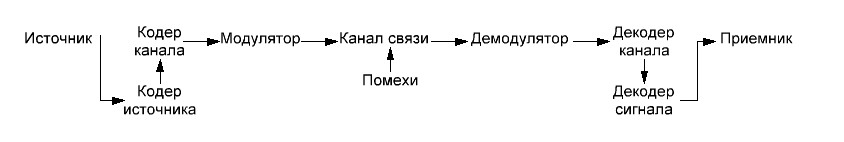
\includegraphics[width=0.9\textwidth]{116_Channel.png}\\
\end{center}
Для повышения помехоустойчивости к передаваемому коду добавляют доп. разряды, при этом число возможных состояний кода увеличивается, однако число информативных состояний остается прежним. То есть часть состояний - запрещенные. Кодовое расстояние - число разрядов из всей совокупности передаваемых кодов, в которых 1 и 0 не совпадают.

Простейшие коды:
\begin{enumerate}
\item добавление контрольного разряда - контроль четности. Двойные ошибки не замечаются, исправление информации невозможно - только контроль правильности.
\item Коды Хэмминга. Кодовое расстояние - 3. Позволяют выявить и исправить одиночную ошибку. Получаются путем объединения по XOR части разрядов числа, но несколько раз.
\item Простой повтор нечетное число раз - по большинству.
\end{enumerate}

При передаче файлами применяется контроль с помощью СRC-кода. Суть: после передачи файла к нему прицепляется контрольная последовательность, получаемая как остаток от деления значения файла на определенный полином, известный и приемнику, и источнику. Полином выбран так, что его значение в квадрате меньше максимального значения файла. Приемник, зная полином, вычисляет свой CRC и сравнивает его с полученным от источника. Если совпадают - передача правильная. Если нет - запрашивается повтор передачи.

Метод наибольшего правдоподобия - по алгоритму Виттерби. Он при приеме предусматривает некоторые ожидаемые стандартные комбинации. В настоящее время применяется в системах цифровой связи.

% Вопрос 117 ----------------------------------------------------------
\section{Приведите основные структуры объединения процессоров в многопроцессорных системах. В чем суть ограничений архитектуры Фон-Неймана.}

Для архитектуры фон Неймана характерны следующие свойства:
\begin{enumerate}
\item единый процессор и единая память
\item линейная организация памяти
\item команды низкого уровня
\item любая операция предусматривает чтение памяти команд, и только затем - обращение к памяти данных. Связь процессора с памятью по ША и ШД.
\end{enumerate}

Реальные проводники из-за своих паразитных характеристик не позволяют передавать сигналы с высокой скоростью, поэтому увеличение производительности за счет повышения тактовой частоты уже почти невозможно. Таким образом, нужны новые структуры ЭВМ.
\begin{enumerate}
\item конвейерная – ряд процессоров, специализированных под конкретные операции, выполняют операции последовательно, передавая результат друг другу. За счет этого может выполняться одновременное преобразование нескольких слов данных. Конвейер реализуется на кристалле, т.к. отдельные блоки объединять накладно.
\item параллельная - объединение нескольких машин через канал. Канал - узкое место. Например, двухмашинный комплекс, в котором вторая машина работает в качестве горячего резерва.
\item иерархическая - один из процессоров выделяется как главный, вспомогательный подключается через блок сопряжения, но при этом теряется универсальность.
\end{enumerate}

Векторно-конвейерные суперкомпьютеры. Конвейер, как последовательное включение процессорных блоков, сохраняется, однако каждый процессорный блок обрабатывает не одно слово данных, а вектор - несколько составленных вместе слов, т.е. в структуре ЭВМ имеются параллельные каналы обработки, соединенные в конвейер. Основная идея - распараллеливание циклического процесса.

Симметричные (SMP) системы - системы с общей памятью. Подключение нескольких процессоров к общей памяти, каждому процессору выделяется буферная память. При этом пока один процессор занимает шину, остальные могут работать с информацией из кэша. С ростом числа процессоров эффективность метода падает, т.к. приходится постоянно наполнять кэш. Замена шины на электронный коммутатор позволяет увеличить скорость передачи и организовать уже несколько одновременных процессов обращения к памяти. 

Структуры с массовым параллелизмом (MPP) - предельный случай SMP, когда каждому процессору выделен свой блок памяти. В структуре те же блоки, но компоновка иная. Например, обмен информацией происходит по пути: память 1 -> кэш 1-го проц. -> коммутатор -> кэш 2-го проц. -> память 2. Раздельная память увеличивает интенсивность обмена процессора со своей памятью, и лишь малое время уходит на обмен между блоками памяти разных процессоров, как правило - после выполнения каких-либо законченных процедур.

\begin{center}
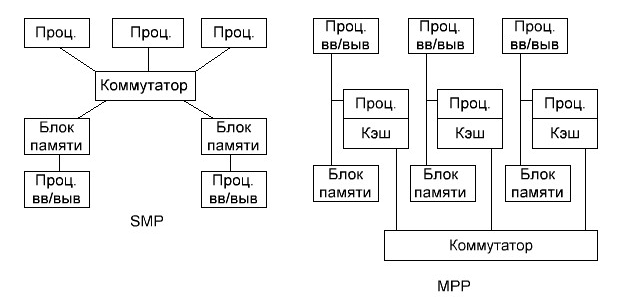
\includegraphics[width=0.8\textwidth]{117_SMP_MPP.png}\\
\end{center}
Кластеры - объединение в единое вычислительное пространство самостоятельных ВС по быстрым сетям. В кластере должен быть управляющий блок - аналог сетевого сервера, по скорости значительно превосходящий остальные узлы. Его задача - распределение и контроль информации.

% Вопрос 118 ----------------------------------------------------------
\section{Сравните структуры двух МПК, имеющих организацию SMP и MPP. Приведите их структурные схемы.}

Симметричные (SMP) системы - системы с общей памятью. Подключение нескольких процессоров к общей памяти требует подключения их к общим шинам адреса и данных. При параллельном подключении процессоров к шине доступ к памяти разрешен только одному - это не увеличивает производительность, поэтому каждому процессору выделяется буферная память. При этом пока один процессор занимает шину, остальные могут работать с информацией из кэша. С ростом числа процессоров эффективность метода падает, т.к. приходится постоянно наполнять кэш. Замена шины на электронный коммутатор позволяет увеличить скорость передачи и организовать уже несколько одновременных процессов обращения к памяти. Адресное пространство для всех общее, но оно распределено по некольким модулям. Каждый процессор преимущественно работает со своим модулем, но может обратиться и к любому другому. Внешние устройства подключаются к блоку памяти или коммутатору через специальные каналы - процессоры ввода/вывода.

Пример SMP системы – "МВК Эльбрус". Общее число процессоров – до 10. Память разделена на 2 логических блока, но адресное пространство общее. Выделяется один управляющий процессор. Развитая система вв\textbackslash выв, так как комплекс должен обслуживать технологическое оборудование.

\begin{center}
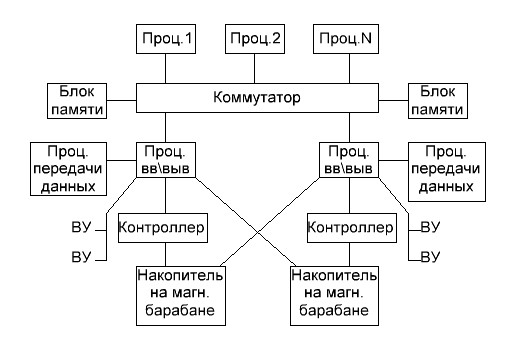
\includegraphics[width=0.7\textwidth]{118_Elbrus.png}
\end{center}
Структуры с массовым параллелизмом (MPP) - предельный случай SMP, когда каждому процессору выделен свой блок памяти. В структуре те же блоки, но компоновка иная. Например, обмен информацией происходит по пути: память 1 ->кэш 1-го проц.->коммутатор->кэш 2-го проц.-> память 2. Раздельная память увеличивает интенсивность обмена процессора со своей памятью, и лишь малое время уходит на обмен между блоками памяти разных процессоров, как правило - после выполнения каких-либо законченных процедур.

С ростом числа процессоров растет сложность коммутаторов. Простейшая структура - матрица. Сложнее - цилиндр, затем - тор (он же - "куб"), соединение кубов - "гиперкуб".

Пример MPP – структуры – МВС-1000. Система 3-го поколения. Размещается в стойках промышленного стандарта. Всего 768 процессоров (по 64 в стойке). В состав системы входят управляющая ЭВМ, файл-сервер, сеть межпроцессорного обмена и FastEthernet. Обязательно – система контроля питания. Коммутатор – двумерный тор.

\begin{center}
\includegraphics[width=0.7\textwidth]{118_MBC-1000.png}
\end{center}
% Вопрос 119 ----------------------------------------------------------
\section{Сравните характеристики двух последовательных интерфейсов RS-232С и USB. Приведите  структурную организацию интерфейсов и формат передаваемых данных.}

RS-232C – последовательная передача по байтам. Формат передачи: стартовый сигнал (1,5-2 такта), 8 разрядов данных от младшего к старшему со строго определенной заранее скоростью, затем контрольный разряд, затем стоповый сигнал и небольшая пауза. Скорости: 2400, 4800, 9600, 19200, 38400.

Для двустороннего обмена достаточно трех проводников – TXD, RXD, GND. Кабель перекручен (TXD источника подключается к RXD приемника, и наоборот). Разъемы COM-порта – DB-25, DB-9. Помимо информационных сигналов, через разъем посылаются сигналы сопровождения – ошибка, готовность.

Интерфейс потенциальный, уровни 0 и 1 передаются уровнями напряжения ±5…15 В. Максимальная длина кабеля – 1,4…1,7 м.

USB – последовательный цепочечный интерфейс с обменом файлами. Частота – 33,6 МГц. Сигналы на линиях – дифференциальные, то есть сигнал распространяется токовый. Размах - ±4 В при питании 5 В. Интерфейс реализуется микросхемой-адаптером с буферной памятью. Обмен между ней и процессором идет с временем цикла процессора, а передача всегда с фиксированной скоростью, то есть для нее нужен собственный тактовый генератор. Время передачи файла соизмеримо с передачей 1 бита по COM-порту. Плата за  скорость - аппаратная часть.

Формат кадра:
\begin{itemize}
\item стартовый импульс
\item адресная часть – 7 бит, адресует до 127 устройств.
\item биты передаваемой информации – число фиксированное, зависит от принятого формата
\item разряды контроля – 5-7 бит – CRC-код.
\item бит конца передачи.
\end{itemize}

Таким образом, передача по кадрам асинхронная, но внутри кадра биты передаются со строго определенной скоростью. В качестве кабеля применяют витую пару (50 Ом). Длина 3…10 м (но рекомендуется не более 5).

% Вопрос 120 ----------------------------------------------------------
\section{Какие принципы программного управления характерны для командного и микро-командного способов управления. В чем сходство и различие этих способов. Покажите на примере структурной схемы устройств управления.}

Принципы программного управления:
\begin{enumerate}
\item Информация кодируется в двоичной форме и разделяется на слова
\item Перед обработкой слова информации исходные данные размещаются в ячейках памяти ЭВМ. Ячейки памяти нумеруются – адреса.
\item Алгоритм обработки представляется в виде последовательности команд - программы. Каждая команда задает ЭВМ тип выполняемой операции и может определять местоположение операндов в памяти ЭВМ указанием  номера ячейки.
\item Команды также кодируются в двоичной форме и располагаются в ячейках памяти ЭВМ
\item Выполнение программы сводится к поочередному выбору команд из памяти ЭВМ и их выполнению. Порядок их выполнения задается алгоритмом и зависит от исходных данных
\end{enumerate}

Три уровня команд:
\begin{enumerate}
\item микрокоманды – элементарное преобразование операнда (пересылка из регистра в регистр, вывод содержимого на выход данных). Микрокоманда выполняется за один такт синхронизации. За время выполнения микрокоманды происходит фиксация входного операнда в регистре процессора (по фронту синхр.) и само преобразование операнда с фиксацией в выходном регистре (по срезу синхр.). Длительность синхросигнала должна быть достаточной для того, чтобы успели закончиться переходные процессы в комбинационных схемах и при записи в регистр.
\item команды – часто приравнивают к операциям. Команда может включать в себя до десятков микрокоманд.
\item макрокоманды (тэги) – появились в силу того, что сложные процедуры требовали большого числа команд, обращений в память. Переход к макрокомандам сокращал их число, повышая скорость выполнения.
\end{enumerate}

Устройство управления с жесткими связями.

Процессор с командным типом управления включает в себя управляющую и операционную части. На вход управляющей поступает КОП, который расшифровывается в сигналы микрокоманд. По результатам текущих операций в управляющую часть возвращаются флаги.
Дешифратор команд выполнен на ПЛМ. Сам пользователь не может изменить ее содержимое.

\begin{center}
\includegraphics[width=0.8\textwidth]{120_microcom.png}
\end{center}
Устройство микропрограммного управления

В его основе лежит введение промежуточного преобразования кода команд в микрокоманды с применением схем памяти. С приходом КОП дешифратор начального адреса микрокоманды формирует адрес, по которому из памяти микрокоманд необходимо считать первую микрокоманду. Считанный код содержит признак смещения, по которому определяется адрес следующей микрокоманды. Замена содержимого памяти микрокоманд эквивалентна замене микрокоманд. Для анализа текущего состояния процессора на схему управления поступают сигналы управления – флаги.

\begin{center}
\includegraphics[width=0.8\textwidth]{120_microprog.png}
\end{center}
\section{Основные понятия процесса проектирования систем управления. Цель процесса проектирования.}
\section{Системный подход к проектированию.}
\section{Структура процесса автоматизированного проектирования.}
\section{Основные типы автоматизированных систем, разновидности САПР.}
\section{Стадии проектирования автоматизированных систем и аспекты их описания.}
\section{Особенности проектирования САПР.}
\section{Понятие о CALS-технологиях.}
\section{Открытые системы.}
\section{Техническое обеспечение систем автоматизированного проектирования.}
\section{Типы сетей, методы доступа в сетях, протоколы и стеки протоколов в вычислительных сетях.}
\section{САПР систем управления.}
\section{Автоматизация управления предприятием, логистические системы.}
\section{АСУТП, автоматизированные системы делопроизводства.}
\section{Математическое обеспечение анализа проектных решений.}
\section{Компоненты математического обеспечения, структура вычислительного процесса анализа.}
\section{Математическое обеспечение анализа на макроуровне.}
\section{Математическое обеспечение анализа на микроуровне.}
\section{Математическое обеспечение анализа на функционально-логическом уровне.}
\section{Математическое обеспечение анализа на системном уровне.}
\section{Математическое обеспечение подсистем машинной графики и геометрического моделирования.}

% Вопрос 141 --------------------------------------------------------
\section{Схемы мультивибратора на транзисторах и ОУ.}

Мультивибратор — генератор колебаний прямоугольной формы с короткими фронтами. Мультивибратор работает в автоколебательном режиме и не имеет устойчивых состояний. По сути представляет собой двухкаскадный резистивный усилитель с глубокой положительной обратной связью. Длительность периода из двух частей равна:

\begin{displaymath}
T = t_1 + t_2 = \ln 2 \cdot R_2 C_1 + \ln 2 \cdot R_3 C_2
\end{displaymath}
\begin{figure}[H]
\centering
\includegraphics[width=0.4\textwidth]{141_tranz.jpg}
\caption{Мультивибратор на транзисторах}
\end{figure}
На ОУ строят мультивибраторы работающие на относительно низких частотах. Для регулировки соотношения длительности положительных и отрицательных импульсов применяется следующая схема (см. рис.).
\begin{figure}[H]
\centering
\includegraphics[width=0.35\textwidth]{141_OU_unsim.jpg}
\caption{Несимметричный мультивибратор на ОУ}
\end{figure}

Время импульса и паузы соответственно:
\begin{displaymath}
t_\text{и} = R_1 C_1 \ln (1 + 2 \frac{R_4}{R_3} )
\end{displaymath}
\begin{displaymath}
t_\text{п} = R_2 C_1 \ln (1 + 2 \frac{R_4}{R_3} )
\end{displaymath}
% Вопрос 142 --------------------------------------------------------
\section{Схема одновибратора на транзисторах.}

Одновибратор - предназначен для формирования прямоугольных импульсов заданной длительности. Имеет одно устойчивое состояние, при котором VT1 закрыт, а VT2 открыт. Длительность генерируемого импульса $T_\text{имп} = 0,7 C_1 R_2 $.

\begin{figure}[H]
\centering
\includegraphics[width=0.4\textwidth]{142.jpg}
\caption{Одновибратор на транзисторах}
\end{figure}

% Вопрос 143 --------------------------------------------------------
\section{Масштабный усилитель на ОУ с К=+10.}

Так как коэффициент усиления положительный, усилитель неинвертирующий:
\begin{figure}[H]
\centering
\includegraphics[width=0.4\textwidth]{143.jpg}
\caption{Масштабный усилитель}
\end{figure}
Коэффициент усиления вычисляется по формуле $K = 1 + \frac{R_2}{R_1} $. Отсюда, для получения коэффициента усиления 10 необходимо, чтобы выполнялось условие $R_2 = (K - 1) R_1 = 9 R_1$. Выбор номиналов зависит от напряжения питания и требуемых токов. Резистор R3, устанавливаемый при необходимости, уменьшает ошибку, возникающую из-за тока смещения, и имеет номинал, равный $R_1 \parallel R_2$.

% Вопрос 144 --------------------------------------------------------
\section{Повторитель на ОУ.}
Рисовать смысла не имеет - просто ОУ со 100\% отрицательной обратной связью. Сигнал поступает на неинвертирующий вход, снимается с выхода. Выходное напряжение равно напряжению на входе, входное сопротивление от 1 MОм до 10 TОм. Повторитель применяется как буферный усилитель, для исключения влияния низкоомной нагрузки на источник с высоким выходным сопротивлением.

% Вопрос 145 --------------------------------------------------------
\section{Двухтактный трансформаторный усилитель мощности, работающий в режиме АВ.}
Транзисторы работают поочередно, каждый во время своего полупериода входного двухполярного сигнала. Для перевода усилителя в режим АВ используются резисторы R1 и R2, создающие напряжение смещения на базах транзисторов (если бы их не было, то были бы искажения типа "ступенька", из-за использования нелинейной части характеристики транзисторов - усилитель работал бы в режиме В).
\begin{figure}[H]
\centering
\includegraphics[width=0.6\textwidth]{145.jpg}
\caption{Двухтактный усилитель мощности}
\end{figure}

% Вопрос 146 --------------------------------------------------------
\section{Избирательные усилители LC и RC.}

Избирательные усилители предназначены для усиления сигналов в узкой полосе частот. По принципу действия различают усилители резонансные и с обратной связью. В резонансных в качестве нагрузки используется колебательный контур, имеющий большое сопротивление на резонансной частоте и малое на остальных. Избирательные свойства оцениваются добротностью $Q = \frac{f_0}{2 \Delta f}$, где $2 \Delta f$ - полоса пропускания.
Усилители с ОС обычно используются на низких частотах. Резонансная частота такого усилителя определяется по формуле $f_0 = \frac{1}{2 \pi R C}$.
\begin{figure}[H]
\centering
\includegraphics[width=0.7\textwidth]{146.jpg}
\caption{Избирательные усилители}
\end{figure}

% Вопрос 147 --------------------------------------------------------
\section{Схема стабилизатора напряжения на 10 В, 2 А на ИС К142.}

Микросхема К142ЕН3 (А, Б) представляет собой регулируемый стабилизатор напряжения с системой защиты от перегрева и перегрузки по току. При срабатывании системы защиты от перегрузки по току, выходное напряжение уменьшается почти до нуля. В случае срабатывания системы тепловой защиты, повторное включение стабилизатора возможно только после остывания микросхемы.

\begin{figure}[H]
\centering
\includegraphics[width=0.6\textwidth]{147.jpg}
\caption{Стабилизатор на 10В, 2А}
\end{figure}

% Вопрос 148 --------------------------------------------------------
\section{Схема стабилизатора напряжения на 12 В, 1 А на ИС К142.}

Требуемым параметрам удовлетворяет микросхема К142ЕН8Б - фиксированное напряжение стабилизации 12 В, ток до 1,5 А.
\begin{figure}[H]
\centering
\includegraphics[width=0.55\textwidth]{148.jpg}
\caption{Стабилизатор на 12В, 1А}
\end{figure}

% Вопрос 149 --------------------------------------------------------
\section{Схема ключевого стабилизатора напряжения.}

Ключевые стабилизаторы напряжения обеспечивают значительно больший КПД за счет того, что транзистор работает в ключевом режиме, то есть потребляет только в открытом состоянии. При этом уменьшаются массогабаритные параметры стабилизатора. Однако, такие стабилизаторы могут стать причиной появления импульсных помех.

Ключевые стабилизаторы содержат накопительную индуктивность, включенную последовательно с нагрузкой. Для сглаживания пульсаций параллельно нагрузке стоит конденсатор. Ключ стоит между источником питания и накопительной индуктивностью. Устройство управления открывает/закрывает ключ в зависимости от напряжения на нагрузке.

При открытом состоянии транзистора напряжение поступает на выход, и одновременно энергия запасается в индуктивности. При отключении транзистора в нагрузке течет ток за счет самоиндукции индуктивности.

\begin{figure}[H]
\centering
\includegraphics[width=0.7\textwidth]{149.jpg}
\caption{Ключевой стабилизатор}
\end{figure}

% Вопрос 150 --------------------------------------------------------
\section{Генератор гармонических колебаний на транзисторах.}

Генераторы гармонических колебаний строятся на основе усилителей с ПОС, обеспечивающих режим самовозбуждения на требуемой частоте. Для работы генератора необходимо выполнение условий баланса амплитуд и баланса фаз.

Генератор LC-типа предназначен для работы в диапазоне десятков кГц и более. Условия генерации здесь создаются на частоте резонанса:
\begin{displaymath}
f_0 = \frac{1}{2 \pi \sqrt{L C}}
\end{displaymath}

Фазовый сдвиг создается соответствующим подключением вторичной обмотки трансформатора. Баланс амплитуд достигается подачей соответствующей амплитуды сигнала с коллекторной нагрузки в цепь базы.

\begin{figure}[H]
\centering
\includegraphics[width=0.45\textwidth]{150_lc.jpg}
\caption{LC-генератор}
\end{figure}

Кроме рассмотренной схемы, широкое распространение получили трехточечные схемы.

\begin{figure}[H]
\centering
\includegraphics[width=0.55\textwidth]{150_3dot.jpg}
\caption{Трехточечные схемы с индуктивной автотрансформаторной (а) и емкостной (б) обратными связями}
\end{figure}

Генератор RC-типа - резистивный усилитель, охваченный ПОС. Для получения фазового сдвига применяются фазовращающие цепочки с несколькими RC-звеньями (минимум 3). Обеспечение условий генерации выполняется подбором элементов в цепи ОС и инверсивными свойствами усилителя.

\begin{figure}[H]
\centering
\includegraphics[width=0.5\textwidth]{150_rc.jpg}
\caption{RC-генератор}
\end{figure}

% Вопрос 151 ----------------------------------------------------------
\section{Системы хранения данных. Назначение. Три основные структуры систем хранения данных.}

С ростом производительности ЭВМ и увеличением объемов хранимой информации возникает необходимость в специальных внешних устройствах для хранения данных. ВЗУ большого объема обычно строятся на основе ленточных накопителей, которые обладают большим временем доступа и быстрым старением. Возникает задача хранения больших объемов данных с быстрым временем доступа.

Причинами появления СХД считают следующие: децентрализация хранения информации (организациям со временем приходится задействовать оборудование филиалов для хранения информации), низкий уровень защиты данных, низкая степень конфиденциальности передаваемых данных, требования к масштабируемости (неизвестно какие объемы информации потребуется хранить через несколько лет). Возникает необходимость в некой автоматизированной системе, которая хранила бы данные.

В простейшем случае структуру такой системы можно представить в следующем виде: \mbox{SCSI --- RAID-контроллер --- HDD (несколько)}.

К SCSI подключается RAID-контроллер с буферным каналом ввода/вывода и кэш-памятью достаточно большого объема. Задача RAID- контроллера обеспечить формирование RAID- массива: присваивание файлам своих адресов. Связь контроллера с HDD осуществляется по параллельным линиям с электрическими или оптическими сигналами.

За счет кэш-памяти RAID-контроллер обеспечивает высокую скорость доступа к данным, при этом задача буферного блока скомпоновать общий файл при нескольких запросах. Кроме того, в буферном блоке производится контроль информации, при необходимости с восстановлением.

Такие СХД подключаются к типовым интерфейсам, прежде всего к SCSI (до 640 Мб/с). Помимо него часто используется Fibre Channel --- интерфейс с оптическими линиями связи способный обеспечивать до 4 Гб/с.

\subsection*{Структура СХД}

Для подключения внешних дисков требуется внешний контроллер с высоким быстродействием, чтобы обеспечить приемлемую скорость передачи массива. Передача идет файлам не непрерывно, с попеременными чтением и записью, поэтому в структуру СХД должны входить следующие блоки:

\begin{figure}[H]
\centering
\includegraphics[width=0.6\textwidth]{151_struct.pdf}
\caption{Структура СХД}
\end{figure}

Процессор контроллера должен обладать высокой переключающей способностью, а интерфейс к ЭВМ должен позволять пересылать большие массивы данных. Связь со стойками с дисками невозможна без буферной памяти.

Информацию при передаче данных можно восстановить, но сбой при записи может привести к потере данных, поэтому система резервируется. Одновременно работают два контроллера, но доступ отдан одному. В случае возникновения ошибки, второй контроллер вступает в работу, его кэш-память так же страхует возможные потери информации.

Такие структуры входят в состав стоек, и часто не одна система хранения данных, а несколько, как бы отдельных.

\subsection*{Организация СХД}

В зависимости от объемов хранимой информации, сложности системы и требований к надежности можно выделить три основные структуры СХД:

\textit{Прямое включение <<DAS>>}. Сервер сети и сервер СХД разделены. Имеется толь одна линия доступа к СХД, что снижает надежность в случае отказа и скорость доступа к данным.

\begin{figure}[H]
\centering
\includegraphics[width=0.4\textwidth]{151_das.pdf}
\caption{Прямое включение <<DAS>>}
\end{figure}

\textit{Прямое подключение в сеть <<NAS>>}. СХД является абонентом сети, обеспечивающим файловый доступ, и должна иметь соответствующее сетевое оборудование. У каждой стойки может быть свое особенное ПО.

\begin{figure}[H]
\centering
\includegraphics[width=0.25\textwidth]{151_nas.pdf}
\caption{Прямое подключение в сеть <<NAS>>}
\end{figure}

\textit{Сетевое подключение <<SAN>>}. Имеется возможность переключения каналов передачи информации. СХД подключается сразу к 2 каналам и, если один из них загружен, то используется второй. Система централизованная, но сложная и дорогая.

\begin{figure}[H]
\centering
\includegraphics[width=0.6\textwidth]{151_san.pdf}
\caption{Сетевое подключение <<SAN>>}
\end{figure}


% Вопрос 152 ----------------------------------------------------------
\section{Основные понятия информационно-вычислительных систем, классификация по критерию потоков информации.}

Понятие вычислительная машина обычно применяют к вычислительному устройству, имеющему небольшие габариты и единую конструкцию. Обычно это устройство включает минимально необходимые функциональные узлы. Система относится к более сложным устройствам и объединяет функциональные блоки территориально разнесенные, чаще однотипные. В составе системы может быть несколько функциональных однотипных блоков. Понятие комплекс выше системы, его применяют к устройствам занимающим определенное пространство, т.е. разнесенные, имеющие каналы связи и разнотипные повторяющиеся функциональные блоки. Поскольку между комплексом и системой граница размыта, обычно их разделяют по конструктивному признаку. \textbf{Комплекс} --- это множество самостоятельных конструктивно устройств. \textbf{Сети} --- территориально разнесенные вычислительные устройства, использующие стандартные способы связи между собой.

Как правило, информационно- вычислительная система (ИВС) или информационно- вычислительный комплекс (ИВК) имеют прикладное назначение. Те или иные конфигурации предназначены для сбора и обработки информации, управления, диагностирования, автоматизированных рабочих мест. В этих структурах непосредственно вычислительные процедуры занимают не основную роль. Основным становится передача, хранение информации. В зависимости от состава системы изменяется конфигурация, динамические характеристики, надежность устройств. В процессе эволюции системы прошли длинный путь, поэтому появились различные конфигурации вычислительных систем.

\textbf{Классификация по потокам информации (по Флину)}

В любой ВС можно выделить два основных информационных потока: поток команд и поток данных, поэтому представляется 4 основных конфигурации:

\begin{enumerate}
\item ОКОД. Один поток команд, один поток данных.

Один процессор с раздельными памятью команд и данных. Это последовательная структура, в которой данные связаны с одной конкретной командой. Если необходимы новые данные, формируется новая команда или повторяется.

\begin{figure}[H]
\centering
\includegraphics[width=0.45\textwidth]{152_okod.pdf}
\caption{Организация ВС: один поток команд, один поток данных}
\end{figure}

\item ОКМД. Один поток команд, множество потоков данных.
\par Специализированные микропроцессоры использующиеся для параллельной обработки различных данных по одной команде. Эта структура наиболее близка к термину параллельная обработка, поскольку в каждый момент времени множество операндов преобразуются под управлением одинаковых команд. Параллельные системы с такой структурой применяют для обработки многомерной графики, сигналов от реальных датчиков, работающих в реальном времени.

\begin{figure}[H]
\centering
\includegraphics[width=0.45\textwidth]{152_okmd.pdf}
\caption{Организация ВС: один поток команд, множество потоков данных}
\end{figure}

\item МКОД. Множество потоков команд, один поток данных.
\par Конвейерная структура реализованная непосредственно на кристалле. Процессоры соединены в цепочку по шинам данных, при этом шины команд у каждого самостоятельные. В каждый момент времени выполняются разные команды в процессорах над одним потоком данных. Поток данных в этом случае --- последовательность операндов несущих информацию о какой-то величине. При этом каждое значение операнда последовательно преобразуется согласно поступающим командам.

\begin{figure}[H]
\centering
\includegraphics[width=0.45\textwidth]{152_mkod.pdf}
\caption{Организация ВС: множество потоков команд, один поток данных}
\end{figure}

\item МКМД. Множество потоков команд, множество потоков данных.
\par Матричная регулярная структура, где матрица процессоров в одном слое использует параллельную обработку, а последовательно по слоям --- конвейер. Такие структуры известны как однородные вычислительные системы. Применяются в сверхбыстродействующих специализированных системах работы с реальными сигналами.

\begin{figure}[H]
\centering
\includegraphics[width=0.45\textwidth]{152_mkmd.pdf}
\caption{Организация ВС: множество потоков команд, множество потоков данных}
\end{figure}

\end{enumerate}


% Вопрос 153 ----------------------------------------------------------
\section{Совмещение операций и многопрограммная работа. Режим работы в реальном времени.}

Режим работы ЭВМ --- это порядок прохождения задач (заданий) через ЭВМ. Задача --- это программа и данные, загруженные в ОП, т.е. программа вместе с выделенными ей ресурсами. Различают режимы работы двух типов --- однозадачный (однопрограммный) и мультизадачный (мультипрограммный).

В \textit{однопрограммном режиме} аппаратура ЭВМ выполняет одну пользовательскую программу под управлением и с использованием программ ОС. Практически это двухпрограммный режим: пользовательская программа плюс программа ОС. Но поскольку программы ОС являются сервисными, обслуживающими запросы пользователя, такой режим называют однопрограммным (однозадачным).

\begin{figure}[H]
\centering
\includegraphics[width=0.5\textwidth]{153_single.pdf}
\caption{Диаграмма загруженности ЭВМ в однопрограммном режиме}
\end{figure}

Основное \textit{достоинство однопрограммного режима} --- минимальное время ответа на запросы пользователя. Все ресурсы ЭВМ (и аппаратные, и программные) находятся в распоряжении пользователя --- нет конкуренции за ресурсы. Пользователь монопольно владеет всеми ресурсами.

Основной \textit{недостаток однопрограммного режима} --- неэффективное использование оборудования, в частности, процессора: как видно из временной диаграммы, большую часть времени процессор простаивает.  Быстродействие системы ввода/вывода, обычно существенно ниже быстродействия процессора и памяти.

Как вариация однопрограммного режима существует \textit{пакетный режим}: в этом режиме пользователь подготавливает последовательность (пакет) запускаемых по очереди программ, что исключает ожидание ввода пользователя для запуска каждой последующей программы. Это несколько повышает реальную производительность системы.

В более мощных, дорогих ЭВМ с целью повышения эффективности использования оборудования применяется \textit{мультипрограммный режим}. В этом режиме, кроме программ ОС, в ОП компьютера располагаются и (по очереди) выполняются несколько (в общем случае М) программ пользователей, при этом, пока одна из программ ожидает завершения операций ввода/вывода, управление передаётся другой программе. Цель --- увеличение загрузки ЦП и, как следствие, производительности ЭВМ.

\begin{figure}[H]
\centering
\includegraphics[width=0.6\textwidth]{153_multi.pdf}
\caption{Диаграмма загруженности ЭВМ в многопрограммном режиме}
\end{figure}

Мультипрограммный режим сложнее однопрограммного, поэтому к ВС предъявляет специальные требования. Для их реализации в состав ЭВМ вводятся специальные средства, которые и принято называть средствами мультипрограммирования. Средства, обеспечивающие заданный режим мультипрограммирования --- это управляющие программы ОС. Они обеспечивают требуемый порядок прохождения задач через ЭВМ, образуют основную часть --- ядро ОС.

\textit{Режим реального времени} применяют в вычислительных системах, работающих с физическими сигналами --- информационно-контролирующими, управляющими, обрабатывающими программами. Понятие это условно, поскольку время изменяется. Условие реального времени $ t_\text{обр.} < t_\text{пер.след.вх.сигн.}$. В этом режиме в первую очередь требуется быстрое измерение сигнала и занесение его в память, поэтому время начала работы процессора определяется временем поступления входного сигнала. Программа запускается по какому-то внешнему событию (чаще прерыванию).


% Вопрос 154 ----------------------------------------------------------
\section{Типы структур многопроцессорных ВС. Параллельные ЭВМ, классификация. Три архитектурных класса машин.}

% Вопрос 155 ----------------------------------------------------------
\section{Принципы ввода-вывода информации в ПЭВМ. Роль и структура контроллера ввода информации.}

Функционирование любого вычислителя складывается из процедур передачи информации между его отдельными функциональными блоками. При этом передача информации между внутренними РОН называется \textit{пересылка}, между процессором и памятью \textit{чтение/запись}, а между памятью и внешними устройствами \textit{ввод/вывод} информации. Наиболее продолжительными по времени процедурами считают операции ввода/вывода, поскольку внешние устройства в большинстве случаев имеют меньшее быстродействие, чем процессор или память, поэтому большое внимание на возможные варианты пересылки информации, рассматривая их с точки зрения снижения времени всей процедуры.

Доступ к внешним устройствам в большинстве случаев адресный, т. е. по структуре ввод/вывод не должен отличаться от чтения/записи. Но объем памяти значителен, значительна и шина адреса (минимум 16 разрядов). В тоже время число внешних устройств не может быть физически большим. В вычислителях системы DEC, i360 было принято ограничение на число внешних устройств 255. Это связано с байтом, хотя реально их значительно меньше. Поэтому, сохраняя адресную выборку ВУ ввод/вывод выполнялся с некоторым отличием  от чтения/записи:
\begin{enumerate}
\item сигналы разрешения ввода/вывода формировались шинным контролером, в то время ОЗУ/ПЗУ блокируется;
\item адрес выставлялся на младшем байте и дублировался на старшем. Старший байт практически не использовался;
\item ШД соединяла выход процессора и вход внешнего устройства (при выводе) и наоборот.
\end{enumerate}

\subsection*{Способы обмена информацией.}

Обмен информацией между внешними устройствами и памятью реализуется в одном из трех подходов:
\begin{enumerate}
\item \textit{Программный режим}.
\par Процессор читает содержимое нужной ячейки памяти ОЗУ и выводит это содержимое (РОН) во внешнее устройство. Не преобразуя информацию процессор выступает лишь как временное хранилище (буферная память). Способ позволяет синхронизировать быстродействие ВУ и памяти. Процедура выполняется за две команды. Адреса на внешнее устройство байтовые. Способ возможен, если в наборе команд имеется команды ввода и вывода.

\item \textit{Ввод/вывод с отображением в память}.
\par Наиболее универсальный способ, применяется, когда нет команд ввода/вывода. Последовательность выполнения та же самая: \mbox{ОЗУ$\rightarrow $CPU, CPU$\rightarrow$ВУ}. Отличие: процессор на внешнее устройство выставляет полный адрес, поэтому из адресного пространства исключаются адреса внешних устройств. Вывод с отображением используется часто, поскольку чтение/запись во многом похожи на ввод/вывод. Основной недостаток второго способа — занимается часть адресного пространства. Поэтому способ рекомендуется, если имеются свободные области в адресном пространстве.

\item \textit{Прямой доступ к памяти (ПДП)}.
\par Суть способа в том, что процессор как бы отключается от ШД и содержимое ОЗУ  напрямую копируется во внешнее устройство. Главная цель применения ПДП — сократить время ввода/вывода с одновременным использованием процессора для выполнения следующей операции. Существует три способа обеспечения режима ПДП:
	\begin{enumerate}
	\item C блокировкой процессора.
	\par С приходом запроса на ПДП, процессор отключается, его выходные шины адреса, данных и управления переводятся в третье состояние. Микрокоманды не расшифровываются устройством управления. Процессор не может выполнять операции, хотя тактовый сигнал и питание поступают. Чтобы перевести процессор в такой режим требуется небольшое время. Для обеспечения управления (сигналы выборки, сопровождения, формирование сигналов адреса) необходимо новое устройство, называемое контролер ПДП. Контролер должен заменить процессор при формировании указанных сигналов. Обратный переход также требует некоторого времени. Способ характерен для несложных микропроцессоров имеющих один или несколько регистров команд и не имеющих внутреннего ОЗУ данных.
	
	\item C квантованием цикла.
	\par В каждом цикле обращения к памяти (ОЗУ, ПЗУ) процессор должен успеть выполнить это обращение за время t/2. Во второй половине цикла процессор отключает свои выходы, позволяя контролеру ПДП выставить свой адрес на шину. За второй интервал выполняется процедура ввода/вывода. Такое условие требует быстродействующей памяти, следовательно, смены элементной базы (переход к ЭСЛ). Последнее затрудняет использование такого подхода, поэтому он практически не применяется.
	
	\item C отъемом цикла.
	\par При работе процессора имеющего внутреннюю буферную память команд и данных реализуется ПДП с отъемом цикла. Процессор начинает команду с выборки — обращение к ПЗУ, далее ОЗУ или ввод/вывод. Третий способ заключается в том, что вместо положенного обращения процессора в память (стандартный цикл) выполняется процедура ввода/вывода режима ПДП. При этом процессор выполняет текущую команду, поскольку в его буфере команд стоит очередь следующих друг за другом команд. Выходные разряды процессора переводятся в третье состояние и не оказывают влияния на состояние шин адреса и данных. Главное отличие от первого способа — процессор выполняет текущую, следующую команды не останавливаясь. Поскольку процессор не занимает шины в этом режиме процедура ввода/вывода выполняется как бы одновременно с основной операцией.
	\end{enumerate}

В любом режиме ПДП необходим контроллер --- специализированная схема работающая синхронно с процессором. Контролеры входят в МП комплекты соответствующих серий. Основу их составляют счетчики адреса с произвольной загрузкой и небольшая схема управления.
\end{enumerate}


% Вопрос 156 ----------------------------------------------------------
\section{Программная реализация ввода чисел с клавиатуры. Привести алгоритм ввода двухразрядного числа с клавиатуры для его суммирования с другими числами.}

Принцип действия универсальной клавиатуры основан на формировании клавиатурного прерывания при нажатии клавиши. Клавиатурное прерывание является внешним и имеет свой вектор. Получив запрос на прерывание, процессор завершает текущую операцию, читает порт клавиатуры (60h) и переписывает код клавиши в буфер клавиатуры, расположенный в области данных BIOS в ОЗУ.

Чтение из буфера можно произвести с помощью стандартных подпрограмм BIOS (int 16h) и DOS (int 21h). В зависимости от подпрограммы процессор читает из буфера один символ (например: mov ah,00h; int 16h) или последовательность символов (например: mov ah,3fh; int 21h).

Т.к. использование таких функций позволяет получить коды символов, то для возможности работы с введенным числом необходимо преобразовать коды символов в двоичный код.  Алгоритм ввода двухразрядного числа для последующей работы с ним ([30h, 39h] — диапазон ASCII-кодов цифр):

Ожидать нажатия клавиши; Сохранить в регистре код нажатой клавиши; Проверить вхождение кода в диапазон [30h, 39h] (если не входит, вывести ошибку, повторить ввод); Отнять от кода 30h; Умножить код на 10; Переслать код в ячейку памяти; Ожидать нажатия клавиши; Сохранить в регистре код нажатой клавиши;  Проверить вхождение кода в диапазон [30h, 39h] (если не входит, вывести ошибку, повторить ввод); Отнять от кода 30h; Прибавить код к содержимому ячейки памяти;


% Вопрос 157 ----------------------------------------------------------
\section{Вывод информации на дисплей. Принципы отображения информации на экране дисплея. LCD-{}дисплеи.}

Мониторы являются наиболее распространённым типом периферийных устройств, входящих в обязательную комплектацию универсальной ЭВМ. Своё наименование они получили по своему принципу работы: периодическое сканирование элементов отображения с текущими изменениями.

Первыми устройствами отображения информации (УОИ) для ЭВМ были точечные индикаторы и индикаторы на основе электронно-лучевой трубки (ЭЛТ). На сегодняшний день применяются устройства на ЭЛТ, на основе жидких кристаллов (ЖК матрицы), плазменные экраны, оптические (голографические) индикаторы, светодиодные экраны.

Любое устройство отображения информации работает с элементами отображения и алфавитом - набором символов, который может отображать устройство. Чем богаче алфавит, тем более качественно монитор представляет информацию. При этом, по способу отображения индикаторы можно разделить на:
\begin{itemize}
\item знакомоделирующие --- каждый знак представляется отдельным символом, поэтому на УОИ мы сразу получаем нужный знак.
\item знакосинтезирующие --- каждый знак строится из нескольких элементов индикации: точек, сегментов, и т.д.
\end{itemize}

Самый простой алфавит --- точка, при этом на его основе можно синтезировать сложные изображения, поэтому точечные индикаторы получили широкое распространение. 

Первые мониторы были монохромными (белый, зелёный цвет). Современные мониторы является цветными, где каждый элемент индикации формируется из трёх точек (красной, зелёной и синей) расположенных рядом друг с другом. За счёт изменения яркости свечения каждой точки изменяется цвет элемента индикации. Потребительскими свойствами мониторов считают величину точки - чем больше точек на единицу длины, тем выше разрешение, четкость изображения. При этом активная точка не должна засвечивать соседей.

ЭЛТ начали применять для отображения информации, т.к. телевизоры уже были, просто нужно было адаптировать их к выводу информации. Однако есть принципиальное отличие - луч ТВ модулируется непрерывным сигналом, в мониторах же представление информации происходит не в реальном времени - следовательно, нужна \underline{экранная память}.

Монитор может работать в символьном или графическом режиме. В \textit{графическом режиме} в память монитора записывается состояние точек (доступ: строка, столбец) и монитор периодически проверяя содержимое памяти обновляет изображение на экране. В \textit{символьном режиме} в память монитора записываются коды символов, которые с помощью знакогенератора преобразуются в символы на экране.

В символьном режиме с помощью точек отображаем символы, поэтому применяется следующий способ: весь экран разбивается на знакоместа. В обычном символьном режиме 25 строк и 80 символов в строке. Чтобы отображать информацию в знакоместах предложена матричная модель знакоместа. Минимальная матрица $5 \times 7$, популярная $7 \times 9$.

Монитор работает не в реальном времени. В общем случае необходима память на все символы экрана. Чтобы увеличить скорость обмена данными вводят дополнительную буферную память. После буферной памяти эти коды преобразуются в управляющие коды луча. Чтобы картинка была стабильной, необходима синхронизация во времени начала движения луча и подачи на модулятор управляющих кодов.

В графическом режиме каждый элемент отображения независим - нет заготовок символов, есть лишь луч, модулятор и точка на луче. Объем экранной памяти значительно возрастает. Чтобы уменьшить объем хранимой в буфере информации используют обработку (точки в линиях, зонах можно хранить не все, а только границы). Не вся информация в кадре меняется - можно переписывать только изменения. Отслеживает это контроллер видеорежима (графический процессор).

\subsection*{LCD-дисплеи}

LCD (Liquid Crystal Display, жидкокристаллические мониторы) основаны на использовании жидких кристаллов - вещества, которое находится в жидком состоянии, но при этом обладает некоторыми свойствами, присущими кристаллическим телам. Фактически, это жидкости, обладающие анизотропией свойств (в частности, оптических), связанных с упорядоченностью в ориентации молекул. Молекулы жидких кристаллов под воздействием электричества могут изменять свои оптические свойства. На этом основан принцип работы LCD-монитора.

ЖК-монитор имеет матричную структуру со строками и столбцами, где в каждой ячейке находится один элемент отображения (пиксель). Каждому элементу отображения соответствует ячейка памяти, где записаны параметры элемента (цвет, яркость). Управление элементами индикации производится подачей сигналов на строки и столбцы. В простейшем случае выбирается столбец, а по строке подаётся сигнал: как следствие элемент на пересечении активен, остальные пассивны.

Конструктивно LCD-матрица представляет многослойную структуру: между двумя слоями очень чистого стекла располагаются элементы отображения, содержащие ЖК, каждый из которых состоит из трёх частей, отвечающих за красный, зелёный и синий цвета. За кристаллами располагается источник света, но пока к кристаллам не приложено электрическое поле свет не проходит за счёт того, что плоскости поляризации неактивного кристалла и поляризационной плёнки на экране перпендикулярны. При приложении электрического поля плоскость поляризации вращается и интенсивность проходящего света увеличивается (в зависимости от угла между плоскостями поляризации плёнки и кристалла от нуля до половины интенсивности источника света). Цвет элемента отображения изменяется в зависимости от интенсивности проходящего света через каждую составляющую элемента индикации (аддитивная модель).

Т.к. источник подсветки общий для всех кристаллов, то имеется неравномерность свечения пикселей (ярче ближе к центру источника). Использование нескольких ламп подсветки снижает неравномерность, а использование множества светодиодных источников (LED-технологии) позволяет получить максимально равномерную подсветку, но стоимость такой подсветки дороже, чем у люминесцентных ламп.

Импульсы активизации элементов должны быть прямоугольными, чтобы обеспечить четкую границу между элементами отображения. Т.к. сигналы передаются по проводнику конечной длины, фронты заваливаются, что приводит к снижению контрастности. Для её повышения применяются матрицы с ключевыми транзисторами, выполненными по пленочной технологии (TFT мониторы).

Основная задача в таких мониторах - сканировать матрицу строка/столбец и одновременно активизировать элементы отображения. Входной видеотракт остался таким же, как в ЭЛТ. Сигналы с него преобразуются в управляющие коды. Синхронизацию по времени осуществляет микропроцессор монитора, отслеживая скорость перемещения информации по строкам/столбцам и начальное сведение сигналов. Контроллер LCD всегда содержит отображение текущего экрана в своей памяти, поэтому он может посылать сигналы без новых входных (удерживать картинку).

Один из недостатков LCD - угол обзора экрана, но эта проблема успешно решается.

% Вопрос 158 ----------------------------------------------------------
\section{Процедура вывода символьной информации на дискретные индикаторы.}

% Вопрос 159 ----------------------------------------------------------
\section{Загрузчики. Процедура загрузки. Статические и динамические загрузки.}

% Вопрос 160 ----------------------------------------------------------
\section{Управление реальной памятью. Виртуальная память. Таблица соответствия адресов.}

В многопрограммном режиме работы возникает задача размещения загружаемых программ в ОЗУ.  Участки памяти, куда загружаются программы, определяются с помощью программы управления памятью — диспетчера памяти. В зависимости от сложности задачи выделяют несколько стратегий управления памятью:

\textit{Статическое деление} --- разделение памяти на участки фиксированного объема, обычно применяется в простейших случаях (2-3 программы). Если процессов много, часть из них должна ожидать своей очереди для размещения в памяти, пока не завершатся предыдущие загруженные программы. Загрузка программы возможна только в том случае, если объем раздела в памяти больше объема программы, следовательно с такой системой загрузки всегда остается неиспользуемое свободное место в памяти, что снижает эффективность ее использования.

\textit{По запросу} --- деление памяти на фрагменты переменной длины. Процессы стоящие в очереди получают необходимый для загрузки объем памяти, следовательно память используется эффективнее. Когда один или несколько процессов завершатся, в освободившуюся область памяти загружаются новые процессы из очереди, которые однако имеют другой размер, поэтому в занимаемой памяти образуются <<дыры>>. Чтобы исправить эту проблему производится \textit{дефрагментация} --- сдвиг одного из массивов к окончанию другого. При этом возникает задача нахождения в кодах абсолютных ссылок и изменения их, для их нахождения команды переходов по абсолютным адресам могут быть отмечены специальным битом (технически это не предусмотрено в системе команд) либо при компиляции в конец файла могут быть записаны адреса таких команд. Для выполнения дефрагментации требуется специальная программа для пересылки массивов.

Другая проблема возникает, когда работающий процесс затребовал дополнительную память, поэтому массив новых данных формируется в другом сегменте памяти. В таком случае программа управления памятью работает как редактор связей: делает ссылку в текущих кодах на новое адресное пространство.

Загрузку программ в память выполняет загрузчик, который выполняет пересылку по необходимым адресам. Загрузка в память выполняется по параграфам (младшая тетрада адреса загрузки равна нулю). Загрузка может производиться в статическом (сначала загружаются все задачи, затем выполняются), либо в динамическом (в промежутках между работой загружаются другие задачи) режимах.

Основная память ВС ограничена, в то же время используя ВЗУ можно попеременно по одним и тем же адресам в основной памяти загружать коды из внешней памяти и работать с ними. Такую организацию памяти называют \textit{виртуальной}. Основная проблема при таком алгоритме работы — связывание конкретной задачи с адресами в ВЗУ. Кроме того, при работе с файлам может возникнуть необходимость сохранения их в ВЗУ, для этого используется таблица соответствия адресов.

\begin{figure}[H]
\centering
\includegraphics[width=0.7\textwidth]{160_virtual_memory.pdf}
\caption{Схема работы с виртуальной памятью}
\end{figure}

\end{document}
